\documentclass[twoside]{book}

% Packages required by doxygen
\usepackage{fixltx2e}
\usepackage{calc}
\usepackage{doxygen}
\usepackage[export]{adjustbox} % also loads graphicx
\usepackage{graphicx}
\usepackage[utf8]{inputenc}
\usepackage{makeidx}
\usepackage{multicol}
\usepackage{multirow}
\PassOptionsToPackage{warn}{textcomp}
\usepackage{textcomp}
\usepackage[nointegrals]{wasysym}
\usepackage[table]{xcolor}

% Font selection
\usepackage[T1]{fontenc}
\usepackage[scaled=.90]{helvet}
\usepackage{courier}
\usepackage{amssymb}
\usepackage{sectsty}
\renewcommand{\familydefault}{\sfdefault}
\allsectionsfont{%
  \fontseries{bc}\selectfont%
  \color{darkgray}%
}
\renewcommand{\DoxyLabelFont}{%
  \fontseries{bc}\selectfont%
  \color{darkgray}%
}
\newcommand{\+}{\discretionary{\mbox{\scriptsize$\hookleftarrow$}}{}{}}

% Page & text layout
\usepackage{geometry}
\geometry{%
  a4paper,%
  top=2.5cm,%
  bottom=2.5cm,%
  left=2.5cm,%
  right=2.5cm%
}
\tolerance=750
\hfuzz=15pt
\hbadness=750
\setlength{\emergencystretch}{15pt}
\setlength{\parindent}{0cm}
\setlength{\parskip}{3ex plus 2ex minus 2ex}
\makeatletter
\renewcommand{\paragraph}{%
  \@startsection{paragraph}{4}{0ex}{-1.0ex}{1.0ex}{%
    \normalfont\normalsize\bfseries\SS@parafont%
  }%
}
\renewcommand{\subparagraph}{%
  \@startsection{subparagraph}{5}{0ex}{-1.0ex}{1.0ex}{%
    \normalfont\normalsize\bfseries\SS@subparafont%
  }%
}
\makeatother

% Headers & footers
\usepackage{fancyhdr}
\pagestyle{fancyplain}
\fancyhead[LE]{\fancyplain{}{\bfseries\thepage}}
\fancyhead[CE]{\fancyplain{}{}}
\fancyhead[RE]{\fancyplain{}{\bfseries\leftmark}}
\fancyhead[LO]{\fancyplain{}{\bfseries\rightmark}}
\fancyhead[CO]{\fancyplain{}{}}
\fancyhead[RO]{\fancyplain{}{\bfseries\thepage}}
\fancyfoot[LE]{\fancyplain{}{}}
\fancyfoot[CE]{\fancyplain{}{}}
\fancyfoot[RE]{\fancyplain{}{\bfseries\scriptsize Generated by Doxygen }}
\fancyfoot[LO]{\fancyplain{}{\bfseries\scriptsize Generated by Doxygen }}
\fancyfoot[CO]{\fancyplain{}{}}
\fancyfoot[RO]{\fancyplain{}{}}
\renewcommand{\footrulewidth}{0.4pt}
\renewcommand{\chaptermark}[1]{%
  \markboth{#1}{}%
}
\renewcommand{\sectionmark}[1]{%
  \markright{\thesection\ #1}%
}

% Indices & bibliography
\usepackage{natbib}
\usepackage[titles]{tocloft}
\setcounter{tocdepth}{3}
\setcounter{secnumdepth}{5}
\makeindex

% Hyperlinks (required, but should be loaded last)
\usepackage{ifpdf}
\ifpdf
  \usepackage[pdftex,pagebackref=true]{hyperref}
\else
  \usepackage[ps2pdf,pagebackref=true]{hyperref}
\fi
\hypersetup{%
  colorlinks=true,%
  linkcolor=blue,%
  citecolor=blue,%
  unicode%
}

% Custom commands
\newcommand{\clearemptydoublepage}{%
  \newpage{\pagestyle{empty}\cleardoublepage}%
}

\usepackage{caption}
\captionsetup{labelsep=space,justification=centering,font={bf},singlelinecheck=off,skip=4pt,position=top}

%===== C O N T E N T S =====

\begin{document}

% Titlepage & ToC
\hypersetup{pageanchor=false,
             bookmarksnumbered=true,
             pdfencoding=unicode
            }
\pagenumbering{alph}
\begin{titlepage}
\vspace*{7cm}
\begin{center}%
{\Large Raytracer \\[1ex]\large 1.\+0.\+0 }\\
\vspace*{1cm}
{\large Generated by Doxygen 1.8.12}\\
\end{center}
\end{titlepage}
\clearemptydoublepage
\pagenumbering{roman}
\tableofcontents
\clearemptydoublepage
\pagenumbering{arabic}
\hypersetup{pageanchor=true}

%--- Begin generated contents ---
\chapter{Module Index}
\section{Modules}
Here is a list of all modules\+:\begin{DoxyCompactList}
\item \contentsline{section}{B\+R\+DF}{\pageref{group___b_r_d_f}}{}
\item \contentsline{section}{Cameras}{\pageref{group___cameras}}{}
\item \contentsline{section}{Geometric\+Objects}{\pageref{group___geometric_objects}}{}
\item \contentsline{section}{Lights}{\pageref{group___lights}}{}
\item \contentsline{section}{Materials}{\pageref{group___materials}}{}
\item \contentsline{section}{Samplers}{\pageref{group___samplers}}{}
\item \contentsline{section}{Tracers}{\pageref{group___tracers}}{}
\item \contentsline{section}{Utilities}{\pageref{group___utilities}}{}
\end{DoxyCompactList}

\chapter{Namespace Index}
\section{Namespace List}
Here is a list of all namespaces with brief descriptions\+:\begin{DoxyCompactList}
\item\contentsline{section}{\hyperlink{namespace_logger}{Logger} }{\pageref{namespace_logger}}{}
\end{DoxyCompactList}

\chapter{Hierarchical Index}
\section{Class Hierarchy}
This inheritance list is sorted roughly, but not completely, alphabetically\+:\begin{DoxyCompactList}
\item \contentsline{section}{B\+R\+DF}{\pageref{class_b_r_d_f}}{}
\begin{DoxyCompactList}
\item \contentsline{section}{Glossy\+Specular}{\pageref{class_glossy_specular}}{}
\item \contentsline{section}{Lambertian}{\pageref{class_lambertian}}{}
\end{DoxyCompactList}
\item \contentsline{section}{Camera}{\pageref{class_camera}}{}
\begin{DoxyCompactList}
\item \contentsline{section}{Orthographic}{\pageref{class_orthographic}}{}
\item \contentsline{section}{Pinhole}{\pageref{class_pinhole}}{}
\item \contentsline{section}{Thin\+Lens}{\pageref{class_thin_lens}}{}
\end{DoxyCompactList}
\item \contentsline{section}{Light}{\pageref{class_light}}{}
\begin{DoxyCompactList}
\item \contentsline{section}{Ambient}{\pageref{class_ambient}}{}
\item \contentsline{section}{Directional}{\pageref{class_directional}}{}
\item \contentsline{section}{Point\+Light}{\pageref{class_point_light}}{}
\end{DoxyCompactList}
\item \contentsline{section}{Material}{\pageref{class_material}}{}
\begin{DoxyCompactList}
\item \contentsline{section}{Matte}{\pageref{class_matte}}{}
\item \contentsline{section}{Phong}{\pageref{class_phong}}{}
\end{DoxyCompactList}
\item \contentsline{section}{Object}{\pageref{class_object}}{}
\begin{DoxyCompactList}
\item \contentsline{section}{Plane}{\pageref{class_plane}}{}
\item \contentsline{section}{Sphere}{\pageref{class_sphere}}{}
\end{DoxyCompactList}
\item \contentsline{section}{Ray}{\pageref{class_ray}}{}
\item \contentsline{section}{R\+G\+B\+Color}{\pageref{class_r_g_b_color}}{}
\item \contentsline{section}{Sampler}{\pageref{class_sampler}}{}
\begin{DoxyCompactList}
\item \contentsline{section}{Hammersley}{\pageref{class_hammersley}}{}
\item \contentsline{section}{Jittered}{\pageref{class_jittered}}{}
\item \contentsline{section}{Multi\+Jittered}{\pageref{class_multi_jittered}}{}
\item \contentsline{section}{N\+Rooks}{\pageref{class_n_rooks}}{}
\item \contentsline{section}{Pure\+Random}{\pageref{class_pure_random}}{}
\item \contentsline{section}{Regular}{\pageref{class_regular}}{}
\end{DoxyCompactList}
\item \contentsline{section}{Surface}{\pageref{class_surface}}{}
\item \contentsline{section}{Tracer}{\pageref{class_tracer}}{}
\begin{DoxyCompactList}
\item \contentsline{section}{Multiple\+Objects}{\pageref{class_multiple_objects}}{}
\item \contentsline{section}{Ray\+Cast}{\pageref{class_ray_cast}}{}
\end{DoxyCompactList}
\end{DoxyCompactList}

\chapter{Class Index}
\section{Class List}
Here are the classes, structs, unions and interfaces with brief descriptions\+:\begin{DoxyCompactList}
\item\contentsline{section}{\hyperlink{class_ambient}{Ambient} }{\pageref{class_ambient}}{}
\item\contentsline{section}{\hyperlink{class_b_r_d_f}{B\+R\+DF} }{\pageref{class_b_r_d_f}}{}
\item\contentsline{section}{\hyperlink{class_camera}{Camera} }{\pageref{class_camera}}{}
\item\contentsline{section}{\hyperlink{class_directional}{Directional} }{\pageref{class_directional}}{}
\item\contentsline{section}{\hyperlink{class_glossy_specular}{Glossy\+Specular} }{\pageref{class_glossy_specular}}{}
\item\contentsline{section}{\hyperlink{class_hammersley}{Hammersley} }{\pageref{class_hammersley}}{}
\item\contentsline{section}{\hyperlink{class_jittered}{Jittered} }{\pageref{class_jittered}}{}
\item\contentsline{section}{\hyperlink{class_lambertian}{Lambertian} }{\pageref{class_lambertian}}{}
\item\contentsline{section}{\hyperlink{class_light}{Light} }{\pageref{class_light}}{}
\item\contentsline{section}{\hyperlink{class_material}{Material} }{\pageref{class_material}}{}
\item\contentsline{section}{\hyperlink{class_matte}{Matte} }{\pageref{class_matte}}{}
\item\contentsline{section}{\hyperlink{class_multi_jittered}{Multi\+Jittered} }{\pageref{class_multi_jittered}}{}
\item\contentsline{section}{\hyperlink{class_multiple_objects}{Multiple\+Objects} }{\pageref{class_multiple_objects}}{}
\item\contentsline{section}{\hyperlink{class_n_rooks}{N\+Rooks} }{\pageref{class_n_rooks}}{}
\item\contentsline{section}{\hyperlink{class_object}{Object} }{\pageref{class_object}}{}
\item\contentsline{section}{\hyperlink{class_orthographic}{Orthographic} }{\pageref{class_orthographic}}{}
\item\contentsline{section}{\hyperlink{class_phong}{Phong} }{\pageref{class_phong}}{}
\item\contentsline{section}{\hyperlink{class_pinhole}{Pinhole} }{\pageref{class_pinhole}}{}
\item\contentsline{section}{\hyperlink{class_plane}{Plane} }{\pageref{class_plane}}{}
\item\contentsline{section}{\hyperlink{class_point_light}{Point\+Light} }{\pageref{class_point_light}}{}
\item\contentsline{section}{\hyperlink{class_pure_random}{Pure\+Random} }{\pageref{class_pure_random}}{}
\item\contentsline{section}{\hyperlink{class_ray}{Ray} }{\pageref{class_ray}}{}
\item\contentsline{section}{\hyperlink{class_ray_cast}{Ray\+Cast} }{\pageref{class_ray_cast}}{}
\item\contentsline{section}{\hyperlink{class_regular}{Regular} }{\pageref{class_regular}}{}
\item\contentsline{section}{\hyperlink{class_r_g_b_color}{R\+G\+B\+Color} }{\pageref{class_r_g_b_color}}{}
\item\contentsline{section}{\hyperlink{class_sampler}{Sampler} }{\pageref{class_sampler}}{}
\item\contentsline{section}{\hyperlink{class_sphere}{Sphere} }{\pageref{class_sphere}}{}
\item\contentsline{section}{\hyperlink{class_surface}{Surface} }{\pageref{class_surface}}{}
\item\contentsline{section}{\hyperlink{class_thin_lens}{Thin\+Lens} }{\pageref{class_thin_lens}}{}
\item\contentsline{section}{\hyperlink{class_tracer}{Tracer} }{\pageref{class_tracer}}{}
\end{DoxyCompactList}

\chapter{File Index}
\section{File List}
Here is a list of all files with brief descriptions\+:\begin{DoxyCompactList}
\item\contentsline{section}{Source/\+B\+R\+D\+Fs/include/\hyperlink{_b_r_d_f_8h}{B\+R\+D\+F.\+h} }{\pageref{_b_r_d_f_8h}}{}
\item\contentsline{section}{Source/\+B\+R\+D\+Fs/include/\hyperlink{_glossy_specular_8h}{Glossy\+Specular.\+h} }{\pageref{_glossy_specular_8h}}{}
\item\contentsline{section}{Source/\+B\+R\+D\+Fs/include/\hyperlink{_lambertian_8h}{Lambertian.\+h} }{\pageref{_lambertian_8h}}{}
\item\contentsline{section}{Source/\+Cameras/include/\hyperlink{_camera_8h}{Camera.\+h} }{\pageref{_camera_8h}}{}
\item\contentsline{section}{Source/\+Cameras/include/\hyperlink{_orthographic_8h}{Orthographic.\+h} }{\pageref{_orthographic_8h}}{}
\item\contentsline{section}{Source/\+Cameras/include/\hyperlink{_pinhole_8h}{Pinhole.\+h} }{\pageref{_pinhole_8h}}{}
\item\contentsline{section}{Source/\+Cameras/include/\hyperlink{_thin_lens_8h}{Thin\+Lens.\+h} }{\pageref{_thin_lens_8h}}{}
\item\contentsline{section}{Source/\+Geometric\+Objects/include/\hyperlink{_object_8h}{Object.\+h} }{\pageref{_object_8h}}{}
\item\contentsline{section}{Source/\+Geometric\+Objects/include/\hyperlink{_plane_8h}{Plane.\+h} }{\pageref{_plane_8h}}{}
\item\contentsline{section}{Source/\+Geometric\+Objects/include/\hyperlink{_sphere_8h}{Sphere.\+h} }{\pageref{_sphere_8h}}{}
\item\contentsline{section}{Source/\+Lights/include/\hyperlink{_ambient_8h}{Ambient.\+h} }{\pageref{_ambient_8h}}{}
\item\contentsline{section}{Source/\+Lights/include/\hyperlink{_directional_8h}{Directional.\+h} }{\pageref{_directional_8h}}{}
\item\contentsline{section}{Source/\+Lights/include/\hyperlink{_light_8h}{Light.\+h} }{\pageref{_light_8h}}{}
\item\contentsline{section}{Source/\+Lights/include/\hyperlink{_point_light_8h}{Point\+Light.\+h} }{\pageref{_point_light_8h}}{}
\item\contentsline{section}{Source/\+Materials/include/\hyperlink{_material_8h}{Material.\+h} }{\pageref{_material_8h}}{}
\item\contentsline{section}{Source/\+Materials/include/\hyperlink{_matte_8h}{Matte.\+h} }{\pageref{_matte_8h}}{}
\item\contentsline{section}{Source/\+Materials/include/\hyperlink{_phong_8h}{Phong.\+h} }{\pageref{_phong_8h}}{}
\item\contentsline{section}{Source/\+Samplers/include/\hyperlink{_hammersley_8h}{Hammersley.\+h} }{\pageref{_hammersley_8h}}{}
\item\contentsline{section}{Source/\+Samplers/include/\hyperlink{_jittered_8h}{Jittered.\+h} }{\pageref{_jittered_8h}}{}
\item\contentsline{section}{Source/\+Samplers/include/\hyperlink{_multi_jittered_8h}{Multi\+Jittered.\+h} }{\pageref{_multi_jittered_8h}}{}
\item\contentsline{section}{Source/\+Samplers/include/\hyperlink{_n_rooks_8h}{N\+Rooks.\+h} }{\pageref{_n_rooks_8h}}{}
\item\contentsline{section}{Source/\+Samplers/include/\hyperlink{_pure_random_8h}{Pure\+Random.\+h} }{\pageref{_pure_random_8h}}{}
\item\contentsline{section}{Source/\+Samplers/include/\hyperlink{_regular_8h}{Regular.\+h} }{\pageref{_regular_8h}}{}
\item\contentsline{section}{Source/\+Samplers/include/\hyperlink{_sampler_8h}{Sampler.\+h} }{\pageref{_sampler_8h}}{}
\item\contentsline{section}{Source/\+Tracers/include/\hyperlink{_multiple_objects_8h}{Multiple\+Objects.\+h} }{\pageref{_multiple_objects_8h}}{}
\item\contentsline{section}{Source/\+Tracers/include/\hyperlink{_ray_cast_8h}{Ray\+Cast.\+h} }{\pageref{_ray_cast_8h}}{}
\item\contentsline{section}{Source/\+Tracers/include/\hyperlink{_tracer_8h}{Tracer.\+h} }{\pageref{_tracer_8h}}{}
\item\contentsline{section}{Source/\+Utilities/include/\hyperlink{_logger_8h}{Logger.\+h} }{\pageref{_logger_8h}}{}
\item\contentsline{section}{Source/\+Utilities/include/\hyperlink{_ray_8h}{Ray.\+h} }{\pageref{_ray_8h}}{}
\item\contentsline{section}{Source/\+Utilities/include/\hyperlink{_r_g_b_color_8h}{R\+G\+B\+Color.\+h} }{\pageref{_r_g_b_color_8h}}{}
\item\contentsline{section}{Source/\+Utilities/include/\hyperlink{_surface_8h}{Surface.\+h} }{\pageref{_surface_8h}}{}
\end{DoxyCompactList}

\chapter{Module Documentation}
\hypertarget{group___b_r_d_f}{}\section{B\+R\+DF}
\label{group___b_r_d_f}\index{B\+R\+DF@{B\+R\+DF}}
\subsection*{Classes}
\begin{DoxyCompactItemize}
\item 
class \hyperlink{class_b_r_d_f}{B\+R\+DF}
\item 
class \hyperlink{class_glossy_specular}{Glossy\+Specular}
\item 
class \hyperlink{class_lambertian}{Lambertian}
\end{DoxyCompactItemize}
\subsection*{Functions}
\begin{DoxyCompactItemize}
\item 
void \hyperlink{group___b_r_d_f_ga77a2a5e48ca3093d853e5713afa01108}{B\+R\+D\+F\+::\+Set\+Sampler} (std\+::shared\+\_\+ptr$<$ \hyperlink{class_sampler}{Sampler} $>$)
\item 
void \hyperlink{group___b_r_d_f_gab7e40f362680b631c40530c9c605e3b3}{Glossy\+Specular\+::\+Set\+Specular\+Reflection} (const float ksr)
\item 
void \hyperlink{group___b_r_d_f_ga4bc78448419beb3d49ae4a9d96a8c5ad}{Glossy\+Specular\+::\+Set\+Specular\+Color} (const \hyperlink{class_r_g_b_color}{R\+G\+B\+Color} \&color)
\item 
void \hyperlink{group___b_r_d_f_ga06b9d29c576be7fcacef68edb57cfc23}{Glossy\+Specular\+::\+Set\+Specular\+Exponent} (const float ksexp)
\item 
virtual \hyperlink{class_r_g_b_color}{R\+G\+B\+Color} \hyperlink{group___b_r_d_f_gad7b8c290aaacbe6c11ee62529dd7389b}{Lambertian\+::f} (const \hyperlink{class_surface}{Surface} \&sr, const glm\+::vec3 \&wi, const glm\+::vec3 \&wo) const
\item 
virtual \hyperlink{class_r_g_b_color}{R\+G\+B\+Color} \hyperlink{group___b_r_d_f_gaa70272886cbeb0f91c629ace938dd0a0}{Lambertian\+::rho} (const \hyperlink{class_surface}{Surface} \&sr, const glm\+::vec3 \&wo) const
\item 
void \hyperlink{group___b_r_d_f_ga4d1bf71e27d8eacc273d244e01fe2d46}{Lambertian\+::\+Set\+Diffuse\+Reflection} (const float kdr)
\item 
void \hyperlink{group___b_r_d_f_gadd1e0590ffcada37b485b985182439de}{Lambertian\+::\+Set\+Diffuse\+Color} (const \hyperlink{class_r_g_b_color}{R\+G\+B\+Color} \&color)
\end{DoxyCompactItemize}


\subsection{Detailed Description}


\subsection{Function Documentation}
\hypertarget{group___b_r_d_f_gad7b8c290aaacbe6c11ee62529dd7389b}{}\label{group___b_r_d_f_gad7b8c290aaacbe6c11ee62529dd7389b} 
\index{B\+R\+DF@{B\+R\+DF}!f@{f}}
\index{f@{f}!B\+R\+DF@{B\+R\+DF}}
\subsubsection{\texorpdfstring{f()}{f()}}
{\footnotesize\ttfamily \hyperlink{class_r_g_b_color}{R\+G\+B\+Color} Lambertian\+::f (\begin{DoxyParamCaption}\item[{const \hyperlink{class_surface}{Surface} \&}]{sr,  }\item[{const glm\+::vec3 \&}]{wi,  }\item[{const glm\+::vec3 \&}]{wo }\end{DoxyParamCaption}) const\hspace{0.3cm}{\ttfamily [inline]}, {\ttfamily [virtual]}}

Computes the reflected radiance along wo. 
\begin{DoxyParams}{Parameters}
{\em sr} & Information about the surface of the object. \\
\hline
{\em wi} & Incoming light direction. \\
\hline
{\em wo} & Reflected light direction. \\
\hline
\end{DoxyParams}
\begin{DoxyReturn}{Returns}
Reflected radiance of a surface. 
\end{DoxyReturn}


Reimplemented from \hyperlink{class_b_r_d_f_af3d87a4237b7b25b72ad1fb5027721bb}{B\+R\+DF}.

\hypertarget{group___b_r_d_f_gaa70272886cbeb0f91c629ace938dd0a0}{}\label{group___b_r_d_f_gaa70272886cbeb0f91c629ace938dd0a0} 
\index{B\+R\+DF@{B\+R\+DF}!rho@{rho}}
\index{rho@{rho}!B\+R\+DF@{B\+R\+DF}}
\subsubsection{\texorpdfstring{rho()}{rho()}}
{\footnotesize\ttfamily \hyperlink{class_r_g_b_color}{R\+G\+B\+Color} Lambertian\+::rho (\begin{DoxyParamCaption}\item[{const \hyperlink{class_surface}{Surface} \&}]{sr,  }\item[{const glm\+::vec3 \&}]{wo }\end{DoxyParamCaption}) const\hspace{0.3cm}{\ttfamily [inline]}, {\ttfamily [virtual]}}

Computes the perfect diffuse reflectance. 
\begin{DoxyParams}{Parameters}
{\em sr} & Information about the surface of the object. \\
\hline
{\em wo} & Reflected light direction. \\
\hline
\end{DoxyParams}
\begin{DoxyReturn}{Returns}
Perfect diffuse reflectance. 
\end{DoxyReturn}


Reimplemented from \hyperlink{class_b_r_d_f_a676438154e142c5762193ee5251e4d57}{B\+R\+DF}.

\hypertarget{group___b_r_d_f_gadd1e0590ffcada37b485b985182439de}{}\label{group___b_r_d_f_gadd1e0590ffcada37b485b985182439de} 
\index{B\+R\+DF@{B\+R\+DF}!Set\+Diffuse\+Color@{Set\+Diffuse\+Color}}
\index{Set\+Diffuse\+Color@{Set\+Diffuse\+Color}!B\+R\+DF@{B\+R\+DF}}
\subsubsection{\texorpdfstring{Set\+Diffuse\+Color()}{SetDiffuseColor()}}
{\footnotesize\ttfamily void Lambertian\+::\+Set\+Diffuse\+Color (\begin{DoxyParamCaption}\item[{const \hyperlink{class_r_g_b_color}{R\+G\+B\+Color} \&}]{color }\end{DoxyParamCaption})\hspace{0.3cm}{\ttfamily [inline]}}

Sets the diffuse color. 
\begin{DoxyParams}{Parameters}
{\em color} & Target diffuse color. \\
\hline
\end{DoxyParams}
\hypertarget{group___b_r_d_f_ga4d1bf71e27d8eacc273d244e01fe2d46}{}\label{group___b_r_d_f_ga4d1bf71e27d8eacc273d244e01fe2d46} 
\index{B\+R\+DF@{B\+R\+DF}!Set\+Diffuse\+Reflection@{Set\+Diffuse\+Reflection}}
\index{Set\+Diffuse\+Reflection@{Set\+Diffuse\+Reflection}!B\+R\+DF@{B\+R\+DF}}
\subsubsection{\texorpdfstring{Set\+Diffuse\+Reflection()}{SetDiffuseReflection()}}
{\footnotesize\ttfamily void Lambertian\+::\+Set\+Diffuse\+Reflection (\begin{DoxyParamCaption}\item[{const float}]{kdr }\end{DoxyParamCaption})\hspace{0.3cm}{\ttfamily [inline]}}

Sets the diffuse reflection coefficient. 
\begin{DoxyParams}{Parameters}
{\em kdr} & Target diffuse reflection coefficient. \\
\hline
\end{DoxyParams}
\hypertarget{group___b_r_d_f_ga77a2a5e48ca3093d853e5713afa01108}{}\label{group___b_r_d_f_ga77a2a5e48ca3093d853e5713afa01108} 
\index{B\+R\+DF@{B\+R\+DF}!Set\+Sampler@{Set\+Sampler}}
\index{Set\+Sampler@{Set\+Sampler}!B\+R\+DF@{B\+R\+DF}}
\subsubsection{\texorpdfstring{Set\+Sampler()}{SetSampler()}}
{\footnotesize\ttfamily void B\+R\+D\+F\+::\+Set\+Sampler (\begin{DoxyParamCaption}\item[{std\+::shared\+\_\+ptr$<$ \hyperlink{class_sampler}{Sampler} $>$}]{sampler\+\_\+ptr }\end{DoxyParamCaption})\hspace{0.3cm}{\ttfamily [inline]}}

Sets a sampler to the \hyperlink{class_b_r_d_f}{B\+R\+DF}. 
\begin{DoxyParams}{Parameters}
{\em sampler\+\_\+ptr} & Target sampler. \\
\hline
\end{DoxyParams}
\hypertarget{group___b_r_d_f_ga4bc78448419beb3d49ae4a9d96a8c5ad}{}\label{group___b_r_d_f_ga4bc78448419beb3d49ae4a9d96a8c5ad} 
\index{B\+R\+DF@{B\+R\+DF}!Set\+Specular\+Color@{Set\+Specular\+Color}}
\index{Set\+Specular\+Color@{Set\+Specular\+Color}!B\+R\+DF@{B\+R\+DF}}
\subsubsection{\texorpdfstring{Set\+Specular\+Color()}{SetSpecularColor()}}
{\footnotesize\ttfamily void Glossy\+Specular\+::\+Set\+Specular\+Color (\begin{DoxyParamCaption}\item[{const \hyperlink{class_r_g_b_color}{R\+G\+B\+Color} \&}]{color }\end{DoxyParamCaption})\hspace{0.3cm}{\ttfamily [inline]}}

Sets the specular color. 
\begin{DoxyParams}{Parameters}
{\em color} & Target specular color. \\
\hline
\end{DoxyParams}
\hypertarget{group___b_r_d_f_ga06b9d29c576be7fcacef68edb57cfc23}{}\label{group___b_r_d_f_ga06b9d29c576be7fcacef68edb57cfc23} 
\index{B\+R\+DF@{B\+R\+DF}!Set\+Specular\+Exponent@{Set\+Specular\+Exponent}}
\index{Set\+Specular\+Exponent@{Set\+Specular\+Exponent}!B\+R\+DF@{B\+R\+DF}}
\subsubsection{\texorpdfstring{Set\+Specular\+Exponent()}{SetSpecularExponent()}}
{\footnotesize\ttfamily void Glossy\+Specular\+::\+Set\+Specular\+Exponent (\begin{DoxyParamCaption}\item[{const float}]{ksexp }\end{DoxyParamCaption})\hspace{0.3cm}{\ttfamily [inline]}}

Sets the specular exponent. 
\begin{DoxyParams}{Parameters}
{\em ksexp} & Target specular exponent. \\
\hline
\end{DoxyParams}
\hypertarget{group___b_r_d_f_gab7e40f362680b631c40530c9c605e3b3}{}\label{group___b_r_d_f_gab7e40f362680b631c40530c9c605e3b3} 
\index{B\+R\+DF@{B\+R\+DF}!Set\+Specular\+Reflection@{Set\+Specular\+Reflection}}
\index{Set\+Specular\+Reflection@{Set\+Specular\+Reflection}!B\+R\+DF@{B\+R\+DF}}
\subsubsection{\texorpdfstring{Set\+Specular\+Reflection()}{SetSpecularReflection()}}
{\footnotesize\ttfamily void Glossy\+Specular\+::\+Set\+Specular\+Reflection (\begin{DoxyParamCaption}\item[{const float}]{ksr }\end{DoxyParamCaption})\hspace{0.3cm}{\ttfamily [inline]}}

Sets the specular reflection coefficient. 
\begin{DoxyParams}{Parameters}
{\em ksr} & Target specular reflection coefficient. \\
\hline
\end{DoxyParams}

\hypertarget{group___cameras}{}\section{Cameras}
\label{group___cameras}\index{Cameras@{Cameras}}
\subsection*{Classes}
\begin{DoxyCompactItemize}
\item 
class \hyperlink{class_camera}{Camera}
\item 
class \hyperlink{class_orthographic}{Orthographic}
\item 
class \hyperlink{class_pinhole}{Pinhole}
\end{DoxyCompactItemize}
\subsection*{Functions}
\begin{DoxyCompactItemize}
\item 
void \hyperlink{group___cameras_gad2265245e85699e077dc1d8d33eecece}{Camera\+::\+Set\+Eye} (const glm\+::vec3 \&eye)
\item 
void \hyperlink{group___cameras_ga92295d79a45f2ab1756221836567997a}{Camera\+::\+Look\+At} (const glm\+::vec3 \&look\+\_\+at)
\item 
void \hyperlink{group___cameras_gaa6c9c847b6db5c4d6450fb9b75f26e81}{Camera\+::\+Set\+Up\+Vector} (const glm\+::vec3 \&up)
\item 
void \hyperlink{group___cameras_ga0e499019f7cd3029602461fcd63aa40c}{Camera\+::\+Set\+Yaw} (const float yaw)
\item 
void \hyperlink{group___cameras_ga33e125b9d164e7332dba4cc01c468d6c}{Camera\+::\+Set\+Pitch} (const float pitch)
\item 
void \hyperlink{group___cameras_ga2c07ac7e812f4dab134fc06692fcaf11}{Camera\+::\+Set\+Roll} (const float roll)
\item 
void \hyperlink{group___cameras_gaf9985918fc0135ac8c98344c96129509}{Camera\+::\+Set\+Exposure\+Time} (const float etime)
\item 
void \hyperlink{group___cameras_ga4ad79de10c562075c049f2e580f48f9f}{Orthographic\+::\+Set\+View\+Plane\+Distance} (const float distance)
\item 
void \hyperlink{group___cameras_ga9a63b65c5228dc43caae0b986ea8d220}{Orthographic\+::\+Set\+Zoom} (const float zoom)
\item 
void \hyperlink{group___cameras_ga2757f00b8e8e778b6792b0c9e0e4052b}{Pinhole\+::\+Set\+View\+Plane\+Distance} (const float distance)
\item 
void \hyperlink{group___cameras_ga9baed583b61d1808867251fa33d4db56}{Pinhole\+::\+Set\+Zoom} (const float zoom)
\end{DoxyCompactItemize}


\subsection{Detailed Description}


\subsection{Function Documentation}
\hypertarget{group___cameras_ga92295d79a45f2ab1756221836567997a}{}\label{group___cameras_ga92295d79a45f2ab1756221836567997a} 
\index{Cameras@{Cameras}!Look\+At@{Look\+At}}
\index{Look\+At@{Look\+At}!Cameras@{Cameras}}
\subsubsection{\texorpdfstring{Look\+At()}{LookAt()}}
{\footnotesize\ttfamily void Camera\+::\+Look\+At (\begin{DoxyParamCaption}\item[{const glm\+::vec3 \&}]{look\+\_\+at }\end{DoxyParamCaption})\hspace{0.3cm}{\ttfamily [inline]}}

Makes the camera look at a given direction. 
\begin{DoxyParams}{Parameters}
{\em look\+\_\+at} & Target look direction. \\
\hline
\end{DoxyParams}
\hypertarget{group___cameras_gaf9985918fc0135ac8c98344c96129509}{}\label{group___cameras_gaf9985918fc0135ac8c98344c96129509} 
\index{Cameras@{Cameras}!Set\+Exposure\+Time@{Set\+Exposure\+Time}}
\index{Set\+Exposure\+Time@{Set\+Exposure\+Time}!Cameras@{Cameras}}
\subsubsection{\texorpdfstring{Set\+Exposure\+Time()}{SetExposureTime()}}
{\footnotesize\ttfamily void Camera\+::\+Set\+Exposure\+Time (\begin{DoxyParamCaption}\item[{const float}]{etime }\end{DoxyParamCaption})\hspace{0.3cm}{\ttfamily [inline]}}

Sets the exposure time. 
\begin{DoxyParams}{Parameters}
{\em etime} & Target exposure time. \\
\hline
\end{DoxyParams}
\hypertarget{group___cameras_gad2265245e85699e077dc1d8d33eecece}{}\label{group___cameras_gad2265245e85699e077dc1d8d33eecece} 
\index{Cameras@{Cameras}!Set\+Eye@{Set\+Eye}}
\index{Set\+Eye@{Set\+Eye}!Cameras@{Cameras}}
\subsubsection{\texorpdfstring{Set\+Eye()}{SetEye()}}
{\footnotesize\ttfamily void Camera\+::\+Set\+Eye (\begin{DoxyParamCaption}\item[{const glm\+::vec3 \&}]{eye }\end{DoxyParamCaption})\hspace{0.3cm}{\ttfamily [inline]}}

Sets the eye location in world coordinates. 
\begin{DoxyParams}{Parameters}
{\em eye} & Target eye location. \\
\hline
\end{DoxyParams}
\hypertarget{group___cameras_ga33e125b9d164e7332dba4cc01c468d6c}{}\label{group___cameras_ga33e125b9d164e7332dba4cc01c468d6c} 
\index{Cameras@{Cameras}!Set\+Pitch@{Set\+Pitch}}
\index{Set\+Pitch@{Set\+Pitch}!Cameras@{Cameras}}
\subsubsection{\texorpdfstring{Set\+Pitch()}{SetPitch()}}
{\footnotesize\ttfamily void Camera\+::\+Set\+Pitch (\begin{DoxyParamCaption}\item[{const float}]{pitch }\end{DoxyParamCaption})\hspace{0.3cm}{\ttfamily [inline]}}

Sets the pitch angle in radians. 
\begin{DoxyParams}{Parameters}
{\em pitch} & Target pitch angle. \\
\hline
\end{DoxyParams}
\hypertarget{group___cameras_ga2c07ac7e812f4dab134fc06692fcaf11}{}\label{group___cameras_ga2c07ac7e812f4dab134fc06692fcaf11} 
\index{Cameras@{Cameras}!Set\+Roll@{Set\+Roll}}
\index{Set\+Roll@{Set\+Roll}!Cameras@{Cameras}}
\subsubsection{\texorpdfstring{Set\+Roll()}{SetRoll()}}
{\footnotesize\ttfamily void Camera\+::\+Set\+Roll (\begin{DoxyParamCaption}\item[{const float}]{roll }\end{DoxyParamCaption})\hspace{0.3cm}{\ttfamily [inline]}}

Sets the roll angle in radians. 
\begin{DoxyParams}{Parameters}
{\em roll} & Target roll angle. \\
\hline
\end{DoxyParams}
\hypertarget{group___cameras_gaa6c9c847b6db5c4d6450fb9b75f26e81}{}\label{group___cameras_gaa6c9c847b6db5c4d6450fb9b75f26e81} 
\index{Cameras@{Cameras}!Set\+Up\+Vector@{Set\+Up\+Vector}}
\index{Set\+Up\+Vector@{Set\+Up\+Vector}!Cameras@{Cameras}}
\subsubsection{\texorpdfstring{Set\+Up\+Vector()}{SetUpVector()}}
{\footnotesize\ttfamily void Camera\+::\+Set\+Up\+Vector (\begin{DoxyParamCaption}\item[{const glm\+::vec3 \&}]{up }\end{DoxyParamCaption})\hspace{0.3cm}{\ttfamily [inline]}}

Sets the world up vector. 
\begin{DoxyParams}{Parameters}
{\em up} & Target up vector. \\
\hline
\end{DoxyParams}
\hypertarget{group___cameras_ga4ad79de10c562075c049f2e580f48f9f}{}\label{group___cameras_ga4ad79de10c562075c049f2e580f48f9f} 
\index{Cameras@{Cameras}!Set\+View\+Plane\+Distance@{Set\+View\+Plane\+Distance}}
\index{Set\+View\+Plane\+Distance@{Set\+View\+Plane\+Distance}!Cameras@{Cameras}}
\subsubsection{\texorpdfstring{Set\+View\+Plane\+Distance()}{SetViewPlaneDistance()}\hspace{0.1cm}{\footnotesize\ttfamily [1/2]}}
{\footnotesize\ttfamily void Orthographic\+::\+Set\+View\+Plane\+Distance (\begin{DoxyParamCaption}\item[{const float}]{distance }\end{DoxyParamCaption})\hspace{0.3cm}{\ttfamily [inline]}}

Sets the distance from the camera to the view plane. 
\begin{DoxyParams}{Parameters}
{\em distance} & Target distance. \\
\hline
\end{DoxyParams}
\hypertarget{group___cameras_ga2757f00b8e8e778b6792b0c9e0e4052b}{}\label{group___cameras_ga2757f00b8e8e778b6792b0c9e0e4052b} 
\index{Cameras@{Cameras}!Set\+View\+Plane\+Distance@{Set\+View\+Plane\+Distance}}
\index{Set\+View\+Plane\+Distance@{Set\+View\+Plane\+Distance}!Cameras@{Cameras}}
\subsubsection{\texorpdfstring{Set\+View\+Plane\+Distance()}{SetViewPlaneDistance()}\hspace{0.1cm}{\footnotesize\ttfamily [2/2]}}
{\footnotesize\ttfamily void Pinhole\+::\+Set\+View\+Plane\+Distance (\begin{DoxyParamCaption}\item[{const float}]{distance }\end{DoxyParamCaption})\hspace{0.3cm}{\ttfamily [inline]}}

Sets the distance from the camera to the view plane. 
\begin{DoxyParams}{Parameters}
{\em distance} & Target distance. \\
\hline
\end{DoxyParams}
\hypertarget{group___cameras_ga0e499019f7cd3029602461fcd63aa40c}{}\label{group___cameras_ga0e499019f7cd3029602461fcd63aa40c} 
\index{Cameras@{Cameras}!Set\+Yaw@{Set\+Yaw}}
\index{Set\+Yaw@{Set\+Yaw}!Cameras@{Cameras}}
\subsubsection{\texorpdfstring{Set\+Yaw()}{SetYaw()}}
{\footnotesize\ttfamily void Camera\+::\+Set\+Yaw (\begin{DoxyParamCaption}\item[{const float}]{yaw }\end{DoxyParamCaption})\hspace{0.3cm}{\ttfamily [inline]}}

Sets the yaw angle in radians. 
\begin{DoxyParams}{Parameters}
{\em yaw} & Target yaw angle. \\
\hline
\end{DoxyParams}
\hypertarget{group___cameras_ga9baed583b61d1808867251fa33d4db56}{}\label{group___cameras_ga9baed583b61d1808867251fa33d4db56} 
\index{Cameras@{Cameras}!Set\+Zoom@{Set\+Zoom}}
\index{Set\+Zoom@{Set\+Zoom}!Cameras@{Cameras}}
\subsubsection{\texorpdfstring{Set\+Zoom()}{SetZoom()}\hspace{0.1cm}{\footnotesize\ttfamily [1/2]}}
{\footnotesize\ttfamily void Pinhole\+::\+Set\+Zoom (\begin{DoxyParamCaption}\item[{const float}]{zoom }\end{DoxyParamCaption})\hspace{0.3cm}{\ttfamily [inline]}}

Sets the zoom factor of the camera. 
\begin{DoxyParams}{Parameters}
{\em zoom} & Target zoom factor. \\
\hline
\end{DoxyParams}
\hypertarget{group___cameras_ga9a63b65c5228dc43caae0b986ea8d220}{}\label{group___cameras_ga9a63b65c5228dc43caae0b986ea8d220} 
\index{Cameras@{Cameras}!Set\+Zoom@{Set\+Zoom}}
\index{Set\+Zoom@{Set\+Zoom}!Cameras@{Cameras}}
\subsubsection{\texorpdfstring{Set\+Zoom()}{SetZoom()}\hspace{0.1cm}{\footnotesize\ttfamily [2/2]}}
{\footnotesize\ttfamily void Orthographic\+::\+Set\+Zoom (\begin{DoxyParamCaption}\item[{const float}]{zoom }\end{DoxyParamCaption})\hspace{0.3cm}{\ttfamily [inline]}}

Sets the zoom factor of the camera. 
\begin{DoxyParams}{Parameters}
{\em zoom} & Target zoom factor. \\
\hline
\end{DoxyParams}

\hypertarget{group___geometric_objects}{}\section{Geometric\+Objects}
\label{group___geometric_objects}\index{Geometric\+Objects@{Geometric\+Objects}}
\subsection*{Classes}
\begin{DoxyCompactItemize}
\item 
class \hyperlink{class_object}{Object}
\item 
class \hyperlink{class_plane}{Plane}
\item 
class \hyperlink{class_sphere}{Sphere}
\end{DoxyCompactItemize}
\subsection*{Functions}
\begin{DoxyCompactItemize}
\item 
std\+::shared\+\_\+ptr$<$ \hyperlink{class_material}{Material} $>$ \hyperlink{group___geometric_objects_ga7ad7172879f1b2fd092561827aa2bbb1}{Object\+::\+Get\+Material} () const
\item 
void \hyperlink{group___geometric_objects_ga74fa63e74026915a261117724303adfc}{Object\+::\+Casts\+Shadows} (bool flag)
\item 
bool \hyperlink{group___geometric_objects_gab4254fb85f166245bb7234f5c5295777}{Object\+::\+Casts\+Shadows} () const
\item 
void \hyperlink{group___geometric_objects_ga8fdaa0574a2046f2e280e6c926f7947d}{Plane\+::\+Set\+Point} (const glm\+::vec3 \&point)
\item 
void \hyperlink{group___geometric_objects_ga50e8800fa3595a6b6fafcda17a77388c}{Plane\+::\+Set\+Normal} (const glm\+::vec3 \&normal)
\item 
void \hyperlink{group___geometric_objects_ga2b8aef309428ea904c75ce3300a71e09}{Sphere\+::\+Set\+Center} (const glm\+::vec3 \&center)
\item 
void \hyperlink{group___geometric_objects_ga0377e69b4a636f542c30c6fa977399e3}{Sphere\+::\+Set\+Radius} (const float radius)
\end{DoxyCompactItemize}


\subsection{Detailed Description}


\subsection{Function Documentation}
\hypertarget{group___geometric_objects_ga74fa63e74026915a261117724303adfc}{}\label{group___geometric_objects_ga74fa63e74026915a261117724303adfc} 
\index{Geometric\+Objects@{Geometric\+Objects}!Casts\+Shadows@{Casts\+Shadows}}
\index{Casts\+Shadows@{Casts\+Shadows}!Geometric\+Objects@{Geometric\+Objects}}
\subsubsection{\texorpdfstring{Casts\+Shadows()}{CastsShadows()}\hspace{0.1cm}{\footnotesize\ttfamily [1/2]}}
{\footnotesize\ttfamily void Object\+::\+Casts\+Shadows (\begin{DoxyParamCaption}\item[{bool}]{flag }\end{DoxyParamCaption})\hspace{0.3cm}{\ttfamily [inline]}}

Sets if the object casts shadows over other objects. 
\begin{DoxyParams}{Parameters}
{\em flag} & Flag that sets if the object casts shadows. \\
\hline
\end{DoxyParams}
\hypertarget{group___geometric_objects_gab4254fb85f166245bb7234f5c5295777}{}\label{group___geometric_objects_gab4254fb85f166245bb7234f5c5295777} 
\index{Geometric\+Objects@{Geometric\+Objects}!Casts\+Shadows@{Casts\+Shadows}}
\index{Casts\+Shadows@{Casts\+Shadows}!Geometric\+Objects@{Geometric\+Objects}}
\subsubsection{\texorpdfstring{Casts\+Shadows()}{CastsShadows()}\hspace{0.1cm}{\footnotesize\ttfamily [2/2]}}
{\footnotesize\ttfamily bool Object\+::\+Casts\+Shadows (\begin{DoxyParamCaption}{ }\end{DoxyParamCaption}) const\hspace{0.3cm}{\ttfamily [inline]}}

Checks if the object casts shadows over other objects. \begin{DoxyReturn}{Returns}
True, if the object casts shadows. 
\end{DoxyReturn}
\hypertarget{group___geometric_objects_ga7ad7172879f1b2fd092561827aa2bbb1}{}\label{group___geometric_objects_ga7ad7172879f1b2fd092561827aa2bbb1} 
\index{Geometric\+Objects@{Geometric\+Objects}!Get\+Material@{Get\+Material}}
\index{Get\+Material@{Get\+Material}!Geometric\+Objects@{Geometric\+Objects}}
\subsubsection{\texorpdfstring{Get\+Material()}{GetMaterial()}}
{\footnotesize\ttfamily std\+::shared\+\_\+ptr$<$ \hyperlink{class_material}{Material} $>$ Object\+::\+Get\+Material (\begin{DoxyParamCaption}{ }\end{DoxyParamCaption}) const\hspace{0.3cm}{\ttfamily [inline]}}

Gets the material of the object. \begin{DoxyReturn}{Returns}
Smart pointer to the material attached to the object. 
\end{DoxyReturn}
\hypertarget{group___geometric_objects_ga2b8aef309428ea904c75ce3300a71e09}{}\label{group___geometric_objects_ga2b8aef309428ea904c75ce3300a71e09} 
\index{Geometric\+Objects@{Geometric\+Objects}!Set\+Center@{Set\+Center}}
\index{Set\+Center@{Set\+Center}!Geometric\+Objects@{Geometric\+Objects}}
\subsubsection{\texorpdfstring{Set\+Center()}{SetCenter()}}
{\footnotesize\ttfamily void Sphere\+::\+Set\+Center (\begin{DoxyParamCaption}\item[{const glm\+::vec3 \&}]{center }\end{DoxyParamCaption})\hspace{0.3cm}{\ttfamily [inline]}}

Sets the center of the sphere. 
\begin{DoxyParams}{Parameters}
{\em center} & Target center. \\
\hline
\end{DoxyParams}
\hypertarget{group___geometric_objects_ga50e8800fa3595a6b6fafcda17a77388c}{}\label{group___geometric_objects_ga50e8800fa3595a6b6fafcda17a77388c} 
\index{Geometric\+Objects@{Geometric\+Objects}!Set\+Normal@{Set\+Normal}}
\index{Set\+Normal@{Set\+Normal}!Geometric\+Objects@{Geometric\+Objects}}
\subsubsection{\texorpdfstring{Set\+Normal()}{SetNormal()}}
{\footnotesize\ttfamily void Plane\+::\+Set\+Normal (\begin{DoxyParamCaption}\item[{const glm\+::vec3 \&}]{normal }\end{DoxyParamCaption})\hspace{0.3cm}{\ttfamily [inline]}}

Sets the normal of the plane. 
\begin{DoxyParams}{Parameters}
{\em normal} & Target normal. \\
\hline
\end{DoxyParams}
\hypertarget{group___geometric_objects_ga8fdaa0574a2046f2e280e6c926f7947d}{}\label{group___geometric_objects_ga8fdaa0574a2046f2e280e6c926f7947d} 
\index{Geometric\+Objects@{Geometric\+Objects}!Set\+Point@{Set\+Point}}
\index{Set\+Point@{Set\+Point}!Geometric\+Objects@{Geometric\+Objects}}
\subsubsection{\texorpdfstring{Set\+Point()}{SetPoint()}}
{\footnotesize\ttfamily void Plane\+::\+Set\+Point (\begin{DoxyParamCaption}\item[{const glm\+::vec3 \&}]{point }\end{DoxyParamCaption})\hspace{0.3cm}{\ttfamily [inline]}}

Sets the point of the plane. 
\begin{DoxyParams}{Parameters}
{\em point} & Target point. \\
\hline
\end{DoxyParams}
\hypertarget{group___geometric_objects_ga0377e69b4a636f542c30c6fa977399e3}{}\label{group___geometric_objects_ga0377e69b4a636f542c30c6fa977399e3} 
\index{Geometric\+Objects@{Geometric\+Objects}!Set\+Radius@{Set\+Radius}}
\index{Set\+Radius@{Set\+Radius}!Geometric\+Objects@{Geometric\+Objects}}
\subsubsection{\texorpdfstring{Set\+Radius()}{SetRadius()}}
{\footnotesize\ttfamily void Sphere\+::\+Set\+Radius (\begin{DoxyParamCaption}\item[{const float}]{radius }\end{DoxyParamCaption})\hspace{0.3cm}{\ttfamily [inline]}}

Sets the radius of the sphere. 
\begin{DoxyParams}{Parameters}
{\em radius} & Target radius. \\
\hline
\end{DoxyParams}

\hypertarget{group___lights}{}\section{Lights}
\label{group___lights}\index{Lights@{Lights}}
\subsection*{Classes}
\begin{DoxyCompactItemize}
\item 
class \hyperlink{class_ambient}{Ambient}
\item 
class \hyperlink{class_directional}{Directional}
\item 
class \hyperlink{class_light}{Light}
\item 
class \hyperlink{class_point_light}{Point\+Light}
\end{DoxyCompactItemize}
\subsection*{Functions}
\begin{DoxyCompactItemize}
\item 
void \hyperlink{group___lights_ga5aefcac18f63a3923320e634daff4f57}{Ambient\+::\+Set\+Intensity} (const float intensity)
\item 
void \hyperlink{group___lights_gaac238172e351af4e5b302b0a006bf719}{Ambient\+::\+Set\+Color} (const \hyperlink{class_r_g_b_color}{R\+G\+B\+Color} \&color)
\item 
void \hyperlink{group___lights_gaa916930bad1e02ef24f89039151be8cd}{Directional\+::\+Set\+Intensity} (const float intensity)
\item 
void \hyperlink{group___lights_ga460c4d38eba389fd8e13d994249bbafc}{Directional\+::\+Set\+Color} (const \hyperlink{class_r_g_b_color}{R\+G\+B\+Color} \&color)
\item 
void \hyperlink{group___lights_ga497358d0a37e4a87d5e24f286695c0a6}{Directional\+::\+Set\+Direction} (const glm\+::vec3 \&direction)
\item 
void \hyperlink{group___lights_ga87d9f95e8a6d77b8fd8383b68daa23ff}{Light\+::\+Casts\+Shadows} (bool flag)
\item 
bool \hyperlink{group___lights_gad1397ab09ba91ed92dbbeb0c8fa8bedc}{Light\+::\+Casts\+Shadows} () const
\item 
void \hyperlink{group___lights_ga1d97c3f6d636899b719d5014f74b3530}{Point\+Light\+::\+Set\+Intensity} (const float intensity)
\item 
void \hyperlink{group___lights_ga27c17e299711f7131091c714b837f619}{Point\+Light\+::\+Set\+Color} (const \hyperlink{class_r_g_b_color}{R\+G\+B\+Color} \&color)
\item 
void \hyperlink{group___lights_ga21b458bf745d4fe52a62e503a4fb3d24}{Point\+Light\+::\+Set\+Position} (const glm\+::vec3 \&position)
\end{DoxyCompactItemize}


\subsection{Detailed Description}


\subsection{Function Documentation}
\hypertarget{group___lights_ga87d9f95e8a6d77b8fd8383b68daa23ff}{}\label{group___lights_ga87d9f95e8a6d77b8fd8383b68daa23ff} 
\index{Lights@{Lights}!Casts\+Shadows@{Casts\+Shadows}}
\index{Casts\+Shadows@{Casts\+Shadows}!Lights@{Lights}}
\subsubsection{\texorpdfstring{Casts\+Shadows()}{CastsShadows()}\hspace{0.1cm}{\footnotesize\ttfamily [1/2]}}
{\footnotesize\ttfamily void Light\+::\+Casts\+Shadows (\begin{DoxyParamCaption}\item[{bool}]{flag }\end{DoxyParamCaption})\hspace{0.3cm}{\ttfamily [inline]}}

Sets if the objects illuminated by the light cast shadows over other objects. 
\begin{DoxyParams}{Parameters}
{\em flag} & Flag that sets if the objects illuminates by the light cast shadows. \\
\hline
\end{DoxyParams}
\hypertarget{group___lights_gad1397ab09ba91ed92dbbeb0c8fa8bedc}{}\label{group___lights_gad1397ab09ba91ed92dbbeb0c8fa8bedc} 
\index{Lights@{Lights}!Casts\+Shadows@{Casts\+Shadows}}
\index{Casts\+Shadows@{Casts\+Shadows}!Lights@{Lights}}
\subsubsection{\texorpdfstring{Casts\+Shadows()}{CastsShadows()}\hspace{0.1cm}{\footnotesize\ttfamily [2/2]}}
{\footnotesize\ttfamily bool Light\+::\+Casts\+Shadows (\begin{DoxyParamCaption}{ }\end{DoxyParamCaption}) const\hspace{0.3cm}{\ttfamily [inline]}}

Checks if the objects illuminated by the light cast shadows over other objects. \begin{DoxyReturn}{Returns}
True, if the objects illuminated by the light cast shadows. 
\end{DoxyReturn}
\hypertarget{group___lights_ga460c4d38eba389fd8e13d994249bbafc}{}\label{group___lights_ga460c4d38eba389fd8e13d994249bbafc} 
\index{Lights@{Lights}!Set\+Color@{Set\+Color}}
\index{Set\+Color@{Set\+Color}!Lights@{Lights}}
\subsubsection{\texorpdfstring{Set\+Color()}{SetColor()}\hspace{0.1cm}{\footnotesize\ttfamily [1/3]}}
{\footnotesize\ttfamily void Directional\+::\+Set\+Color (\begin{DoxyParamCaption}\item[{const \hyperlink{class_r_g_b_color}{R\+G\+B\+Color} \&}]{color }\end{DoxyParamCaption})\hspace{0.3cm}{\ttfamily [inline]}}

Sets the color of the light. 
\begin{DoxyParams}{Parameters}
{\em color} & Target color. \\
\hline
\end{DoxyParams}
\hypertarget{group___lights_ga27c17e299711f7131091c714b837f619}{}\label{group___lights_ga27c17e299711f7131091c714b837f619} 
\index{Lights@{Lights}!Set\+Color@{Set\+Color}}
\index{Set\+Color@{Set\+Color}!Lights@{Lights}}
\subsubsection{\texorpdfstring{Set\+Color()}{SetColor()}\hspace{0.1cm}{\footnotesize\ttfamily [2/3]}}
{\footnotesize\ttfamily void Point\+Light\+::\+Set\+Color (\begin{DoxyParamCaption}\item[{const \hyperlink{class_r_g_b_color}{R\+G\+B\+Color} \&}]{color }\end{DoxyParamCaption})\hspace{0.3cm}{\ttfamily [inline]}}

Sets the color of the light. 
\begin{DoxyParams}{Parameters}
{\em color} & Target color. \\
\hline
\end{DoxyParams}
\hypertarget{group___lights_gaac238172e351af4e5b302b0a006bf719}{}\label{group___lights_gaac238172e351af4e5b302b0a006bf719} 
\index{Lights@{Lights}!Set\+Color@{Set\+Color}}
\index{Set\+Color@{Set\+Color}!Lights@{Lights}}
\subsubsection{\texorpdfstring{Set\+Color()}{SetColor()}\hspace{0.1cm}{\footnotesize\ttfamily [3/3]}}
{\footnotesize\ttfamily void Ambient\+::\+Set\+Color (\begin{DoxyParamCaption}\item[{const \hyperlink{class_r_g_b_color}{R\+G\+B\+Color} \&}]{color }\end{DoxyParamCaption})\hspace{0.3cm}{\ttfamily [inline]}}

Sets the color of the light. 
\begin{DoxyParams}{Parameters}
{\em color} & Target color. \\
\hline
\end{DoxyParams}
\hypertarget{group___lights_ga497358d0a37e4a87d5e24f286695c0a6}{}\label{group___lights_ga497358d0a37e4a87d5e24f286695c0a6} 
\index{Lights@{Lights}!Set\+Direction@{Set\+Direction}}
\index{Set\+Direction@{Set\+Direction}!Lights@{Lights}}
\subsubsection{\texorpdfstring{Set\+Direction()}{SetDirection()}}
{\footnotesize\ttfamily void Directional\+::\+Set\+Direction (\begin{DoxyParamCaption}\item[{const glm\+::vec3 \&}]{direction }\end{DoxyParamCaption})\hspace{0.3cm}{\ttfamily [inline]}}

Sets the direction of the light. 
\begin{DoxyParams}{Parameters}
{\em direction} & Target direction. \\
\hline
\end{DoxyParams}
\hypertarget{group___lights_ga1d97c3f6d636899b719d5014f74b3530}{}\label{group___lights_ga1d97c3f6d636899b719d5014f74b3530} 
\index{Lights@{Lights}!Set\+Intensity@{Set\+Intensity}}
\index{Set\+Intensity@{Set\+Intensity}!Lights@{Lights}}
\subsubsection{\texorpdfstring{Set\+Intensity()}{SetIntensity()}\hspace{0.1cm}{\footnotesize\ttfamily [1/3]}}
{\footnotesize\ttfamily void Point\+Light\+::\+Set\+Intensity (\begin{DoxyParamCaption}\item[{const float}]{intensity }\end{DoxyParamCaption})\hspace{0.3cm}{\ttfamily [inline]}}

Sets the intensity of the light. 
\begin{DoxyParams}{Parameters}
{\em intensity} & Target intensity. \\
\hline
\end{DoxyParams}
\hypertarget{group___lights_ga5aefcac18f63a3923320e634daff4f57}{}\label{group___lights_ga5aefcac18f63a3923320e634daff4f57} 
\index{Lights@{Lights}!Set\+Intensity@{Set\+Intensity}}
\index{Set\+Intensity@{Set\+Intensity}!Lights@{Lights}}
\subsubsection{\texorpdfstring{Set\+Intensity()}{SetIntensity()}\hspace{0.1cm}{\footnotesize\ttfamily [2/3]}}
{\footnotesize\ttfamily void Ambient\+::\+Set\+Intensity (\begin{DoxyParamCaption}\item[{const float}]{intensity }\end{DoxyParamCaption})\hspace{0.3cm}{\ttfamily [inline]}}

Sets the intensity of the light. 
\begin{DoxyParams}{Parameters}
{\em intensity} & Target intensity. \\
\hline
\end{DoxyParams}
\hypertarget{group___lights_gaa916930bad1e02ef24f89039151be8cd}{}\label{group___lights_gaa916930bad1e02ef24f89039151be8cd} 
\index{Lights@{Lights}!Set\+Intensity@{Set\+Intensity}}
\index{Set\+Intensity@{Set\+Intensity}!Lights@{Lights}}
\subsubsection{\texorpdfstring{Set\+Intensity()}{SetIntensity()}\hspace{0.1cm}{\footnotesize\ttfamily [3/3]}}
{\footnotesize\ttfamily void Directional\+::\+Set\+Intensity (\begin{DoxyParamCaption}\item[{const float}]{intensity }\end{DoxyParamCaption})\hspace{0.3cm}{\ttfamily [inline]}}

Sets the intensity of the light. 
\begin{DoxyParams}{Parameters}
{\em intensity} & Target intensity. \\
\hline
\end{DoxyParams}
\hypertarget{group___lights_ga21b458bf745d4fe52a62e503a4fb3d24}{}\label{group___lights_ga21b458bf745d4fe52a62e503a4fb3d24} 
\index{Lights@{Lights}!Set\+Position@{Set\+Position}}
\index{Set\+Position@{Set\+Position}!Lights@{Lights}}
\subsubsection{\texorpdfstring{Set\+Position()}{SetPosition()}}
{\footnotesize\ttfamily void Point\+Light\+::\+Set\+Position (\begin{DoxyParamCaption}\item[{const glm\+::vec3 \&}]{position }\end{DoxyParamCaption})\hspace{0.3cm}{\ttfamily [inline]}}

Sets the position of the light in world coordinates. 
\begin{DoxyParams}{Parameters}
{\em position} & Target position. \\
\hline
\end{DoxyParams}

\hypertarget{group___materials}{}\section{Materials}
\label{group___materials}\index{Materials@{Materials}}
\subsection*{Classes}
\begin{DoxyCompactItemize}
\item 
class \hyperlink{class_material}{Material}
\item 
class \hyperlink{class_matte}{Matte}
\item 
class \hyperlink{class_phong}{Phong}
\end{DoxyCompactItemize}
\subsection*{Functions}
\begin{DoxyCompactItemize}
\item 
void \hyperlink{group___materials_gad4df0e4b6f2112282b492f068faf1d72}{Matte\+::\+Set\+Ambient\+Reflection} (const float kdr)
\item 
void \hyperlink{group___materials_ga3a3fb682a6cfb419d05bf5dba9088f57}{Matte\+::\+Set\+Ambient\+Color} (const \hyperlink{class_r_g_b_color}{R\+G\+B\+Color} \&color)
\item 
void \hyperlink{group___materials_ga59c2ccdf9e80053784f5449603c7b7a3}{Matte\+::\+Set\+Diffuse\+Reflection} (const float kdr)
\item 
void \hyperlink{group___materials_ga6a82d5d8fd47aeb188380c067477e396}{Matte\+::\+Set\+Diffuse\+Color} (const \hyperlink{class_r_g_b_color}{R\+G\+B\+Color} \&color)
\item 
void \hyperlink{group___materials_ga6b42d7c8b02c61801702dc19d8e3ba5a}{Matte\+::\+Set\+Sampler} (std\+::shared\+\_\+ptr$<$ \hyperlink{class_sampler}{Sampler} $>$ sampler\+\_\+ptr)
\item 
void \hyperlink{group___materials_ga245b163a849cf378e84ed77620172f74}{Phong\+::\+Set\+Ambient\+Reflection} (const float kdr)
\item 
void \hyperlink{group___materials_ga7562b2e0139a3e2e93e61954d13c281f}{Phong\+::\+Set\+Ambient\+Color} (const \hyperlink{class_r_g_b_color}{R\+G\+B\+Color} \&color)
\item 
void \hyperlink{group___materials_ga7d9198210719a327b6c293955a9ecafe}{Phong\+::\+Set\+Diffuse\+Reflection} (const float kdr)
\item 
void \hyperlink{group___materials_ga54c0c1a1b40732588660aebbe01ce94f}{Phong\+::\+Set\+Diffuse\+Color} (const \hyperlink{class_r_g_b_color}{R\+G\+B\+Color} \&color)
\item 
void \hyperlink{group___materials_gaaa0823035fefb08e6f20e4af9c6f73d2}{Phong\+::\+Set\+Specular\+Reflection} (const float kdr)
\item 
void \hyperlink{group___materials_gaed8372d4e59cb7c1b781979c4ea9ee80}{Phong\+::\+Set\+Specular\+Color} (const \hyperlink{class_r_g_b_color}{R\+G\+B\+Color} \&color)
\item 
void \hyperlink{group___materials_ga167d70d514005d94a0bede7d7b12f372}{Phong\+::\+Set\+Specular\+Exponent} (const float ksexp)
\item 
void \hyperlink{group___materials_ga76b02c8e5a8dfff0a24c929b37a47c0c}{Phong\+::\+Set\+Sampler} (std\+::shared\+\_\+ptr$<$ \hyperlink{class_sampler}{Sampler} $>$)
\end{DoxyCompactItemize}


\subsection{Detailed Description}


\subsection{Function Documentation}
\hypertarget{group___materials_ga3a3fb682a6cfb419d05bf5dba9088f57}{}\label{group___materials_ga3a3fb682a6cfb419d05bf5dba9088f57} 
\index{Materials@{Materials}!Set\+Ambient\+Color@{Set\+Ambient\+Color}}
\index{Set\+Ambient\+Color@{Set\+Ambient\+Color}!Materials@{Materials}}
\subsubsection{\texorpdfstring{Set\+Ambient\+Color()}{SetAmbientColor()}\hspace{0.1cm}{\footnotesize\ttfamily [1/2]}}
{\footnotesize\ttfamily void Matte\+::\+Set\+Ambient\+Color (\begin{DoxyParamCaption}\item[{const \hyperlink{class_r_g_b_color}{R\+G\+B\+Color} \&}]{color }\end{DoxyParamCaption})\hspace{0.3cm}{\ttfamily [inline]}}

Sets the diffuse color of the ambient component of the material. 
\begin{DoxyParams}{Parameters}
{\em color} & Target diffuse color. \\
\hline
\end{DoxyParams}
\hypertarget{group___materials_ga7562b2e0139a3e2e93e61954d13c281f}{}\label{group___materials_ga7562b2e0139a3e2e93e61954d13c281f} 
\index{Materials@{Materials}!Set\+Ambient\+Color@{Set\+Ambient\+Color}}
\index{Set\+Ambient\+Color@{Set\+Ambient\+Color}!Materials@{Materials}}
\subsubsection{\texorpdfstring{Set\+Ambient\+Color()}{SetAmbientColor()}\hspace{0.1cm}{\footnotesize\ttfamily [2/2]}}
{\footnotesize\ttfamily void Phong\+::\+Set\+Ambient\+Color (\begin{DoxyParamCaption}\item[{const \hyperlink{class_r_g_b_color}{R\+G\+B\+Color} \&}]{color }\end{DoxyParamCaption})\hspace{0.3cm}{\ttfamily [inline]}}

Sets the diffuse color of the ambient component of the material. 
\begin{DoxyParams}{Parameters}
{\em color} & Target diffuse color. \\
\hline
\end{DoxyParams}
\hypertarget{group___materials_gad4df0e4b6f2112282b492f068faf1d72}{}\label{group___materials_gad4df0e4b6f2112282b492f068faf1d72} 
\index{Materials@{Materials}!Set\+Ambient\+Reflection@{Set\+Ambient\+Reflection}}
\index{Set\+Ambient\+Reflection@{Set\+Ambient\+Reflection}!Materials@{Materials}}
\subsubsection{\texorpdfstring{Set\+Ambient\+Reflection()}{SetAmbientReflection()}\hspace{0.1cm}{\footnotesize\ttfamily [1/2]}}
{\footnotesize\ttfamily void Matte\+::\+Set\+Ambient\+Reflection (\begin{DoxyParamCaption}\item[{const float}]{kdr }\end{DoxyParamCaption})\hspace{0.3cm}{\ttfamily [inline]}}

Sets the diffuse reflection of the ambient component of the material. 
\begin{DoxyParams}{Parameters}
{\em kdr} & Target diffuse reflection. \\
\hline
\end{DoxyParams}
\hypertarget{group___materials_ga245b163a849cf378e84ed77620172f74}{}\label{group___materials_ga245b163a849cf378e84ed77620172f74} 
\index{Materials@{Materials}!Set\+Ambient\+Reflection@{Set\+Ambient\+Reflection}}
\index{Set\+Ambient\+Reflection@{Set\+Ambient\+Reflection}!Materials@{Materials}}
\subsubsection{\texorpdfstring{Set\+Ambient\+Reflection()}{SetAmbientReflection()}\hspace{0.1cm}{\footnotesize\ttfamily [2/2]}}
{\footnotesize\ttfamily void Phong\+::\+Set\+Ambient\+Reflection (\begin{DoxyParamCaption}\item[{const float}]{kdr }\end{DoxyParamCaption})\hspace{0.3cm}{\ttfamily [inline]}}

Sets the diffuse reflection of the ambient component of the material. 
\begin{DoxyParams}{Parameters}
{\em kdr} & Target diffuse reflection. \\
\hline
\end{DoxyParams}
\hypertarget{group___materials_ga6a82d5d8fd47aeb188380c067477e396}{}\label{group___materials_ga6a82d5d8fd47aeb188380c067477e396} 
\index{Materials@{Materials}!Set\+Diffuse\+Color@{Set\+Diffuse\+Color}}
\index{Set\+Diffuse\+Color@{Set\+Diffuse\+Color}!Materials@{Materials}}
\subsubsection{\texorpdfstring{Set\+Diffuse\+Color()}{SetDiffuseColor()}\hspace{0.1cm}{\footnotesize\ttfamily [1/2]}}
{\footnotesize\ttfamily void Matte\+::\+Set\+Diffuse\+Color (\begin{DoxyParamCaption}\item[{const \hyperlink{class_r_g_b_color}{R\+G\+B\+Color} \&}]{color }\end{DoxyParamCaption})\hspace{0.3cm}{\ttfamily [inline]}}

Sets the diffuse color of the diffuse component of the material. 
\begin{DoxyParams}{Parameters}
{\em color} & Target diffuse color. \\
\hline
\end{DoxyParams}
\hypertarget{group___materials_ga54c0c1a1b40732588660aebbe01ce94f}{}\label{group___materials_ga54c0c1a1b40732588660aebbe01ce94f} 
\index{Materials@{Materials}!Set\+Diffuse\+Color@{Set\+Diffuse\+Color}}
\index{Set\+Diffuse\+Color@{Set\+Diffuse\+Color}!Materials@{Materials}}
\subsubsection{\texorpdfstring{Set\+Diffuse\+Color()}{SetDiffuseColor()}\hspace{0.1cm}{\footnotesize\ttfamily [2/2]}}
{\footnotesize\ttfamily void Phong\+::\+Set\+Diffuse\+Color (\begin{DoxyParamCaption}\item[{const \hyperlink{class_r_g_b_color}{R\+G\+B\+Color} \&}]{color }\end{DoxyParamCaption})\hspace{0.3cm}{\ttfamily [inline]}}

Sets the diffuse color of the diffuse component of the material. 
\begin{DoxyParams}{Parameters}
{\em color} & Target diffuse color. \\
\hline
\end{DoxyParams}
\hypertarget{group___materials_ga59c2ccdf9e80053784f5449603c7b7a3}{}\label{group___materials_ga59c2ccdf9e80053784f5449603c7b7a3} 
\index{Materials@{Materials}!Set\+Diffuse\+Reflection@{Set\+Diffuse\+Reflection}}
\index{Set\+Diffuse\+Reflection@{Set\+Diffuse\+Reflection}!Materials@{Materials}}
\subsubsection{\texorpdfstring{Set\+Diffuse\+Reflection()}{SetDiffuseReflection()}\hspace{0.1cm}{\footnotesize\ttfamily [1/2]}}
{\footnotesize\ttfamily void Matte\+::\+Set\+Diffuse\+Reflection (\begin{DoxyParamCaption}\item[{const float}]{kdr }\end{DoxyParamCaption})\hspace{0.3cm}{\ttfamily [inline]}}

Sets the diffuse reflection of the diffuse component of the material. 
\begin{DoxyParams}{Parameters}
{\em kdr} & Target diffuse reflection. \\
\hline
\end{DoxyParams}
\hypertarget{group___materials_ga7d9198210719a327b6c293955a9ecafe}{}\label{group___materials_ga7d9198210719a327b6c293955a9ecafe} 
\index{Materials@{Materials}!Set\+Diffuse\+Reflection@{Set\+Diffuse\+Reflection}}
\index{Set\+Diffuse\+Reflection@{Set\+Diffuse\+Reflection}!Materials@{Materials}}
\subsubsection{\texorpdfstring{Set\+Diffuse\+Reflection()}{SetDiffuseReflection()}\hspace{0.1cm}{\footnotesize\ttfamily [2/2]}}
{\footnotesize\ttfamily void Phong\+::\+Set\+Diffuse\+Reflection (\begin{DoxyParamCaption}\item[{const float}]{kdr }\end{DoxyParamCaption})\hspace{0.3cm}{\ttfamily [inline]}}

Sets the diffuse reflection of the diffuse component of the material. 
\begin{DoxyParams}{Parameters}
{\em kdr} & Target diffuse reflection. \\
\hline
\end{DoxyParams}
\hypertarget{group___materials_ga6b42d7c8b02c61801702dc19d8e3ba5a}{}\label{group___materials_ga6b42d7c8b02c61801702dc19d8e3ba5a} 
\index{Materials@{Materials}!Set\+Sampler@{Set\+Sampler}}
\index{Set\+Sampler@{Set\+Sampler}!Materials@{Materials}}
\subsubsection{\texorpdfstring{Set\+Sampler()}{SetSampler()}\hspace{0.1cm}{\footnotesize\ttfamily [1/2]}}
{\footnotesize\ttfamily void Matte\+::\+Set\+Sampler (\begin{DoxyParamCaption}\item[{std\+::shared\+\_\+ptr$<$ \hyperlink{class_sampler}{Sampler} $>$}]{sampler\+\_\+ptr }\end{DoxyParamCaption})\hspace{0.3cm}{\ttfamily [inline]}}

Sets the sampler to be used by the B\+R\+D\+Fs of the material. 
\begin{DoxyParams}{Parameters}
{\em sampler\+\_\+ptr} & Target sampler. \\
\hline
\end{DoxyParams}
\hypertarget{group___materials_ga76b02c8e5a8dfff0a24c929b37a47c0c}{}\label{group___materials_ga76b02c8e5a8dfff0a24c929b37a47c0c} 
\index{Materials@{Materials}!Set\+Sampler@{Set\+Sampler}}
\index{Set\+Sampler@{Set\+Sampler}!Materials@{Materials}}
\subsubsection{\texorpdfstring{Set\+Sampler()}{SetSampler()}\hspace{0.1cm}{\footnotesize\ttfamily [2/2]}}
{\footnotesize\ttfamily void Phong\+::\+Set\+Sampler (\begin{DoxyParamCaption}\item[{std\+::shared\+\_\+ptr$<$ \hyperlink{class_sampler}{Sampler} $>$}]{sampler\+\_\+ptr }\end{DoxyParamCaption})\hspace{0.3cm}{\ttfamily [inline]}}

Sets the sampler to be used by the B\+R\+D\+Fs of the material. 
\begin{DoxyParams}{Parameters}
{\em sampler\+\_\+ptr} & Target sampler. \\
\hline
\end{DoxyParams}
\hypertarget{group___materials_gaed8372d4e59cb7c1b781979c4ea9ee80}{}\label{group___materials_gaed8372d4e59cb7c1b781979c4ea9ee80} 
\index{Materials@{Materials}!Set\+Specular\+Color@{Set\+Specular\+Color}}
\index{Set\+Specular\+Color@{Set\+Specular\+Color}!Materials@{Materials}}
\subsubsection{\texorpdfstring{Set\+Specular\+Color()}{SetSpecularColor()}}
{\footnotesize\ttfamily void Phong\+::\+Set\+Specular\+Color (\begin{DoxyParamCaption}\item[{const \hyperlink{class_r_g_b_color}{R\+G\+B\+Color} \&}]{color }\end{DoxyParamCaption})\hspace{0.3cm}{\ttfamily [inline]}}

Sets the specular color of the specular component of the material. 
\begin{DoxyParams}{Parameters}
{\em color} & Target specular color. \\
\hline
\end{DoxyParams}
\hypertarget{group___materials_ga167d70d514005d94a0bede7d7b12f372}{}\label{group___materials_ga167d70d514005d94a0bede7d7b12f372} 
\index{Materials@{Materials}!Set\+Specular\+Exponent@{Set\+Specular\+Exponent}}
\index{Set\+Specular\+Exponent@{Set\+Specular\+Exponent}!Materials@{Materials}}
\subsubsection{\texorpdfstring{Set\+Specular\+Exponent()}{SetSpecularExponent()}}
{\footnotesize\ttfamily void Phong\+::\+Set\+Specular\+Exponent (\begin{DoxyParamCaption}\item[{const float}]{ksexp }\end{DoxyParamCaption})\hspace{0.3cm}{\ttfamily [inline]}}

Sets the specular factor of the specular component of the material. 
\begin{DoxyParams}{Parameters}
{\em ksexp} & Target specular factor. \\
\hline
\end{DoxyParams}
\hypertarget{group___materials_gaaa0823035fefb08e6f20e4af9c6f73d2}{}\label{group___materials_gaaa0823035fefb08e6f20e4af9c6f73d2} 
\index{Materials@{Materials}!Set\+Specular\+Reflection@{Set\+Specular\+Reflection}}
\index{Set\+Specular\+Reflection@{Set\+Specular\+Reflection}!Materials@{Materials}}
\subsubsection{\texorpdfstring{Set\+Specular\+Reflection()}{SetSpecularReflection()}}
{\footnotesize\ttfamily void Phong\+::\+Set\+Specular\+Reflection (\begin{DoxyParamCaption}\item[{const float}]{kdr }\end{DoxyParamCaption})\hspace{0.3cm}{\ttfamily [inline]}}

Sets the specular reflection of the specular component of the material. 
\begin{DoxyParams}{Parameters}
{\em kdr} & Target specular reflection. \\
\hline
\end{DoxyParams}

\hypertarget{group___samplers}{}\section{Samplers}
\label{group___samplers}\index{Samplers@{Samplers}}
\subsection*{Classes}
\begin{DoxyCompactItemize}
\item 
class \hyperlink{class_hammersley}{Hammersley}
\item 
class \hyperlink{class_jittered}{Jittered}
\item 
class \hyperlink{class_multi_jittered}{Multi\+Jittered}
\item 
class \hyperlink{class_n_rooks}{N\+Rooks}
\item 
class \hyperlink{class_pure_random}{Pure\+Random}
\item 
class \hyperlink{class_regular}{Regular}
\item 
class \hyperlink{class_sampler}{Sampler}
\end{DoxyCompactItemize}
\subsection*{Functions}
\begin{DoxyCompactItemize}
\item 
int \hyperlink{group___samplers_ga3d438d62d7b7eaec05cff684f96cfe02}{Sampler\+::\+Get\+Num\+Of\+Samples} () const
\end{DoxyCompactItemize}


\subsection{Detailed Description}


\subsection{Function Documentation}
\hypertarget{group___samplers_ga3d438d62d7b7eaec05cff684f96cfe02}{}\label{group___samplers_ga3d438d62d7b7eaec05cff684f96cfe02} 
\index{Samplers@{Samplers}!Get\+Num\+Of\+Samples@{Get\+Num\+Of\+Samples}}
\index{Get\+Num\+Of\+Samples@{Get\+Num\+Of\+Samples}!Samplers@{Samplers}}
\subsubsection{\texorpdfstring{Get\+Num\+Of\+Samples()}{GetNumOfSamples()}}
{\footnotesize\ttfamily int Sampler\+::\+Get\+Num\+Of\+Samples (\begin{DoxyParamCaption}{ }\end{DoxyParamCaption}) const\hspace{0.3cm}{\ttfamily [inline]}}

Returns the number of samples of the sampler. \begin{DoxyReturn}{Returns}
Number of samples. 
\end{DoxyReturn}

\hypertarget{group___tracers}{}\section{Tracers}
\label{group___tracers}\index{Tracers@{Tracers}}
\subsection*{Classes}
\begin{DoxyCompactItemize}
\item 
class \hyperlink{class_ray_cast}{Ray\+Cast}
\item 
class \hyperlink{class_tracer}{Tracer}
\end{DoxyCompactItemize}


\subsection{Detailed Description}

\hypertarget{group___utilities}{}\section{Utilities}
\label{group___utilities}\index{Utilities@{Utilities}}
\subsection*{Namespaces}
\begin{DoxyCompactItemize}
\item 
 \hyperlink{namespace_logger}{Logger}
\end{DoxyCompactItemize}
\subsection*{Classes}
\begin{DoxyCompactItemize}
\item 
class \hyperlink{class_ray}{Ray}
\item 
class \hyperlink{class_r_g_b_color}{R\+G\+B\+Color}
\item 
class \hyperlink{class_surface}{Surface}
\end{DoxyCompactItemize}
\subsection*{Functions}
\begin{DoxyCompactItemize}
\item 
bool \hyperlink{group___utilities_ga51f2ca82bd3166f19e7327c8e5e5a068}{R\+G\+B\+Color\+::operator==} (const \hyperlink{class_r_g_b_color}{R\+G\+B\+Color} \&rhs) const
\item 
\hyperlink{class_r_g_b_color}{R\+G\+B\+Color} \hyperlink{group___utilities_gab8eb3021ce94a9a4fc7a1ba1e8c06a30}{R\+G\+B\+Color\+::operator+} (const \hyperlink{class_r_g_b_color}{R\+G\+B\+Color} \&rhs) const
\item 
\hyperlink{class_r_g_b_color}{R\+G\+B\+Color} \hyperlink{group___utilities_ga2d0a70444ca0c882f3a5dbed42787ef8}{R\+G\+B\+Color\+::operator-\/} (const \hyperlink{class_r_g_b_color}{R\+G\+B\+Color} \&rhs) const
\item 
\hyperlink{class_r_g_b_color}{R\+G\+B\+Color} \hyperlink{group___utilities_ga38cb49925dc77a366b56b546b7dd17ae}{R\+G\+B\+Color\+::operator$\ast$} (const \hyperlink{class_r_g_b_color}{R\+G\+B\+Color} \&rhs) const
\item 
\hyperlink{class_r_g_b_color}{R\+G\+B\+Color} \hyperlink{group___utilities_ga46707b8ca0c4b560914f2aae4ec31eb5}{R\+G\+B\+Color\+::operator$\ast$} (const float rhs) const
\item 
\hyperlink{class_r_g_b_color}{R\+G\+B\+Color} \hyperlink{group___utilities_ga932f5821d1c40799b6b40f2fe88b7070}{R\+G\+B\+Color\+::operator/} (const float rhs) const
\item 
\hyperlink{class_r_g_b_color}{R\+G\+B\+Color} \hyperlink{group___utilities_ga985586cc676498527d1597ab3beee728}{R\+G\+B\+Color\+::operator+=} (const \hyperlink{class_r_g_b_color}{R\+G\+B\+Color} \&rhs)
\item 
\hyperlink{class_r_g_b_color}{R\+G\+B\+Color} \hyperlink{group___utilities_ga1a36960da5c88b5e3e825ad01845de29}{R\+G\+B\+Color\+::operator-\/=} (const \hyperlink{class_r_g_b_color}{R\+G\+B\+Color} \&rhs)
\item 
\hyperlink{class_r_g_b_color}{R\+G\+B\+Color} \hyperlink{group___utilities_ga1b8ab73352d66c6d0125d6f061a1982f}{R\+G\+B\+Color\+::operator$\ast$=} (const float rhs)
\item 
\hyperlink{class_r_g_b_color}{R\+G\+B\+Color} \hyperlink{group___utilities_gad071890eadae01f96bf3af8ba52503e0}{R\+G\+B\+Color\+::operator/=} (const float rhs)
\item 
float \hyperlink{group___utilities_gaea22cae2344d4a4187b50732820e50c8}{R\+G\+B\+Color\+::\+Average} () const
\end{DoxyCompactItemize}


\subsection{Detailed Description}


\subsection{Function Documentation}
\hypertarget{group___utilities_gaea22cae2344d4a4187b50732820e50c8}{}\label{group___utilities_gaea22cae2344d4a4187b50732820e50c8} 
\index{Utilities@{Utilities}!Average@{Average}}
\index{Average@{Average}!Utilities@{Utilities}}
\subsubsection{\texorpdfstring{Average()}{Average()}}
{\footnotesize\ttfamily float R\+G\+B\+Color\+::\+Average (\begin{DoxyParamCaption}{ }\end{DoxyParamCaption}) const\hspace{0.3cm}{\ttfamily [inline]}}

Returns the average of the components of the color. \begin{DoxyReturn}{Returns}
The resulting average of the components of the color. 
\end{DoxyReturn}
\hypertarget{group___utilities_ga38cb49925dc77a366b56b546b7dd17ae}{}\label{group___utilities_ga38cb49925dc77a366b56b546b7dd17ae} 
\index{Utilities@{Utilities}!operator$\ast$@{operator$\ast$}}
\index{operator$\ast$@{operator$\ast$}!Utilities@{Utilities}}
\subsubsection{\texorpdfstring{operator$\ast$()}{operator*()}\hspace{0.1cm}{\footnotesize\ttfamily [1/2]}}
{\footnotesize\ttfamily \hyperlink{class_r_g_b_color}{R\+G\+B\+Color} R\+G\+B\+Color\+::operator$\ast$ (\begin{DoxyParamCaption}\item[{const \hyperlink{class_r_g_b_color}{R\+G\+B\+Color} \&}]{rhs }\end{DoxyParamCaption}) const\hspace{0.3cm}{\ttfamily [inline]}}

Multiplies two colors componentwise. 
\begin{DoxyParams}{Parameters}
{\em rhs} & Right hand side operand. \\
\hline
\end{DoxyParams}
\begin{DoxyReturn}{Returns}
The resulting color of the componentwise multiplication of two colors. 
\end{DoxyReturn}
\hypertarget{group___utilities_ga46707b8ca0c4b560914f2aae4ec31eb5}{}\label{group___utilities_ga46707b8ca0c4b560914f2aae4ec31eb5} 
\index{Utilities@{Utilities}!operator$\ast$@{operator$\ast$}}
\index{operator$\ast$@{operator$\ast$}!Utilities@{Utilities}}
\subsubsection{\texorpdfstring{operator$\ast$()}{operator*()}\hspace{0.1cm}{\footnotesize\ttfamily [2/2]}}
{\footnotesize\ttfamily \hyperlink{class_r_g_b_color}{R\+G\+B\+Color} R\+G\+B\+Color\+::operator$\ast$ (\begin{DoxyParamCaption}\item[{const float}]{rhs }\end{DoxyParamCaption}) const\hspace{0.3cm}{\ttfamily [inline]}}

Multiplies a color by a number. 
\begin{DoxyParams}{Parameters}
{\em rhs} & Right hand side operand. \\
\hline
\end{DoxyParams}
\begin{DoxyReturn}{Returns}
The resulting color of the product of a color by a number. 
\end{DoxyReturn}
\hypertarget{group___utilities_ga1b8ab73352d66c6d0125d6f061a1982f}{}\label{group___utilities_ga1b8ab73352d66c6d0125d6f061a1982f} 
\index{Utilities@{Utilities}!operator$\ast$=@{operator$\ast$=}}
\index{operator$\ast$=@{operator$\ast$=}!Utilities@{Utilities}}
\subsubsection{\texorpdfstring{operator$\ast$=()}{operator*=()}}
{\footnotesize\ttfamily \hyperlink{class_r_g_b_color}{R\+G\+B\+Color} R\+G\+B\+Color\+::operator$\ast$= (\begin{DoxyParamCaption}\item[{const float}]{rhs }\end{DoxyParamCaption})\hspace{0.3cm}{\ttfamily [inline]}}

Multiplies a color by a number and assigns the result to the left operand. 
\begin{DoxyParams}{Parameters}
{\em rhs} & Right hand side operand. \\
\hline
\end{DoxyParams}
\begin{DoxyReturn}{Returns}
The resulting color of the product of a color by a number. 
\end{DoxyReturn}
\hypertarget{group___utilities_gab8eb3021ce94a9a4fc7a1ba1e8c06a30}{}\label{group___utilities_gab8eb3021ce94a9a4fc7a1ba1e8c06a30} 
\index{Utilities@{Utilities}!operator+@{operator+}}
\index{operator+@{operator+}!Utilities@{Utilities}}
\subsubsection{\texorpdfstring{operator+()}{operator+()}}
{\footnotesize\ttfamily \hyperlink{class_r_g_b_color}{R\+G\+B\+Color} R\+G\+B\+Color\+::operator+ (\begin{DoxyParamCaption}\item[{const \hyperlink{class_r_g_b_color}{R\+G\+B\+Color} \&}]{rhs }\end{DoxyParamCaption}) const\hspace{0.3cm}{\ttfamily [inline]}}

Adds two colors componentwise. 
\begin{DoxyParams}{Parameters}
{\em rhs} & Right hand side operand. \\
\hline
\end{DoxyParams}
\begin{DoxyReturn}{Returns}
The resulting color of the componentwise sum of two colors. 
\end{DoxyReturn}
\hypertarget{group___utilities_ga985586cc676498527d1597ab3beee728}{}\label{group___utilities_ga985586cc676498527d1597ab3beee728} 
\index{Utilities@{Utilities}!operator+=@{operator+=}}
\index{operator+=@{operator+=}!Utilities@{Utilities}}
\subsubsection{\texorpdfstring{operator+=()}{operator+=()}}
{\footnotesize\ttfamily \hyperlink{class_r_g_b_color}{R\+G\+B\+Color} R\+G\+B\+Color\+::operator+= (\begin{DoxyParamCaption}\item[{const \hyperlink{class_r_g_b_color}{R\+G\+B\+Color} \&}]{rhs }\end{DoxyParamCaption})\hspace{0.3cm}{\ttfamily [inline]}}

Adds two colors componentwise and assigns the result to the left operand. 
\begin{DoxyParams}{Parameters}
{\em rhs} & Right hand side operand. \\
\hline
\end{DoxyParams}
\begin{DoxyReturn}{Returns}
The resulting color of the componentwise sum of two colors. 
\end{DoxyReturn}
\hypertarget{group___utilities_ga2d0a70444ca0c882f3a5dbed42787ef8}{}\label{group___utilities_ga2d0a70444ca0c882f3a5dbed42787ef8} 
\index{Utilities@{Utilities}!operator-\/@{operator-\/}}
\index{operator-\/@{operator-\/}!Utilities@{Utilities}}
\subsubsection{\texorpdfstring{operator-\/()}{operator-()}}
{\footnotesize\ttfamily \hyperlink{class_r_g_b_color}{R\+G\+B\+Color} R\+G\+B\+Color\+::operator-\/ (\begin{DoxyParamCaption}\item[{const \hyperlink{class_r_g_b_color}{R\+G\+B\+Color} \&}]{rhs }\end{DoxyParamCaption}) const\hspace{0.3cm}{\ttfamily [inline]}}

Substracts two colors componentwise. 
\begin{DoxyParams}{Parameters}
{\em rhs} & Right hand side operand. \\
\hline
\end{DoxyParams}
\begin{DoxyReturn}{Returns}
The resulting color of the componentwise subtraction of two colors. 
\end{DoxyReturn}
\hypertarget{group___utilities_ga1a36960da5c88b5e3e825ad01845de29}{}\label{group___utilities_ga1a36960da5c88b5e3e825ad01845de29} 
\index{Utilities@{Utilities}!operator-\/=@{operator-\/=}}
\index{operator-\/=@{operator-\/=}!Utilities@{Utilities}}
\subsubsection{\texorpdfstring{operator-\/=()}{operator-=()}}
{\footnotesize\ttfamily \hyperlink{class_r_g_b_color}{R\+G\+B\+Color} R\+G\+B\+Color\+::operator-\/= (\begin{DoxyParamCaption}\item[{const \hyperlink{class_r_g_b_color}{R\+G\+B\+Color} \&}]{rhs }\end{DoxyParamCaption})\hspace{0.3cm}{\ttfamily [inline]}}

Substracts two colors componentwise and assigns the result to the left operand. 
\begin{DoxyParams}{Parameters}
{\em rhs} & Right hand side operand. \\
\hline
\end{DoxyParams}
\begin{DoxyReturn}{Returns}
The resulting color of the componentwise subtraction of two colors. 
\end{DoxyReturn}
\hypertarget{group___utilities_ga932f5821d1c40799b6b40f2fe88b7070}{}\label{group___utilities_ga932f5821d1c40799b6b40f2fe88b7070} 
\index{Utilities@{Utilities}!operator/@{operator/}}
\index{operator/@{operator/}!Utilities@{Utilities}}
\subsubsection{\texorpdfstring{operator/()}{operator/()}}
{\footnotesize\ttfamily \hyperlink{class_r_g_b_color}{R\+G\+B\+Color} R\+G\+B\+Color\+::operator/ (\begin{DoxyParamCaption}\item[{const float}]{rhs }\end{DoxyParamCaption}) const\hspace{0.3cm}{\ttfamily [inline]}}

Divides a color by a number. 
\begin{DoxyParams}{Parameters}
{\em rhs} & Right hand side operand. \\
\hline
\end{DoxyParams}
\begin{DoxyReturn}{Returns}
The resulting color of the division of a color by a number. 
\end{DoxyReturn}
\hypertarget{group___utilities_gad071890eadae01f96bf3af8ba52503e0}{}\label{group___utilities_gad071890eadae01f96bf3af8ba52503e0} 
\index{Utilities@{Utilities}!operator/=@{operator/=}}
\index{operator/=@{operator/=}!Utilities@{Utilities}}
\subsubsection{\texorpdfstring{operator/=()}{operator/=()}}
{\footnotesize\ttfamily \hyperlink{class_r_g_b_color}{R\+G\+B\+Color} R\+G\+B\+Color\+::operator/= (\begin{DoxyParamCaption}\item[{const float}]{rhs }\end{DoxyParamCaption})\hspace{0.3cm}{\ttfamily [inline]}}

Divides a color by a number and assigns the result to the left operand. 
\begin{DoxyParams}{Parameters}
{\em rhs} & Right hand side operand. \\
\hline
\end{DoxyParams}
\begin{DoxyReturn}{Returns}
The resulting color of the division of a color by a number. 
\end{DoxyReturn}
\hypertarget{group___utilities_ga51f2ca82bd3166f19e7327c8e5e5a068}{}\label{group___utilities_ga51f2ca82bd3166f19e7327c8e5e5a068} 
\index{Utilities@{Utilities}!operator==@{operator==}}
\index{operator==@{operator==}!Utilities@{Utilities}}
\subsubsection{\texorpdfstring{operator==()}{operator==()}}
{\footnotesize\ttfamily bool R\+G\+B\+Color\+::operator== (\begin{DoxyParamCaption}\item[{const \hyperlink{class_r_g_b_color}{R\+G\+B\+Color} \&}]{rhs }\end{DoxyParamCaption}) const\hspace{0.3cm}{\ttfamily [inline]}}

Checks if the components of two colors are equal. 
\begin{DoxyParams}{Parameters}
{\em rhs} & Right hand side operand. \\
\hline
\end{DoxyParams}
\begin{DoxyReturn}{Returns}
A boolean value indicating whether the two colors are equal. 
\end{DoxyReturn}

\chapter{Namespace Documentation}
\hypertarget{namespace_logger}{}\section{Logger Namespace Reference}
\label{namespace_logger}\index{Logger@{Logger}}
\subsection*{Enumerations}
\begin{DoxyCompactItemize}
\item 
enum \hyperlink{namespace_logger_a8f625bd9ec5f706cb67b725a98743c04}{Log\+Type} \{ \hyperlink{namespace_logger_a8f625bd9ec5f706cb67b725a98743c04ab46e195aa1062a5d9f4366486ea131f3}{L\+T\+\_\+\+D\+E\+B\+UG}, 
\hyperlink{namespace_logger_a8f625bd9ec5f706cb67b725a98743c04a7558ebf8aecb9a3b538e639e11237f33}{L\+T\+\_\+\+E\+R\+R\+OR}, 
\hyperlink{namespace_logger_a8f625bd9ec5f706cb67b725a98743c04ae2f929c9ea7ffc45e696e247034a1616}{L\+T\+\_\+\+I\+N\+FO}
 \}
\item 
enum \hyperlink{namespace_logger_a5838bb966bb2e56b838cbf5ce207d014}{Log\+Detail} \{ \hyperlink{namespace_logger_a5838bb966bb2e56b838cbf5ce207d014a13b85f16e10f02f0f7831f7f1e62172e}{L\+D\+\_\+\+L\+I\+T\+T\+LE}, 
\hyperlink{namespace_logger_a5838bb966bb2e56b838cbf5ce207d014acdb9720161dbe34ef066448bc3362452}{L\+D\+\_\+\+N\+O\+R\+M\+AL}, 
\hyperlink{namespace_logger_a5838bb966bb2e56b838cbf5ce207d014a81011f9c7cb8f58acfae6d88b064466b}{L\+D\+\_\+\+H\+I\+GH}
 \}
\item 
enum \hyperlink{namespace_logger_ac0ba8933d14b2c05d8a87ef9319924fa}{Log\+Relevance} \{ \hyperlink{namespace_logger_ac0ba8933d14b2c05d8a87ef9319924faaae660d03b3378eb8cf44d6acc5f03734}{L\+R\+\_\+\+T\+R\+I\+V\+I\+AL}, 
\hyperlink{namespace_logger_ac0ba8933d14b2c05d8a87ef9319924faa4427eed1049860091a1cd794be6817cf}{L\+R\+\_\+\+N\+O\+R\+M\+AL}, 
\hyperlink{namespace_logger_ac0ba8933d14b2c05d8a87ef9319924faa34fddfe05472d43cf2f67c5ecae54d57}{L\+R\+\_\+\+I\+M\+P\+O\+R\+T\+A\+NT}
 \}
\end{DoxyCompactItemize}
\subsection*{Functions}
\begin{DoxyCompactItemize}
\item 
void \hyperlink{namespace_logger_aea870326f4476cc49457cfdcc6256022}{Start\+Log} ()
\item 
void \hyperlink{namespace_logger_a6506657f7b715f4ed4de8545c9b44e44}{Log} (\hyperlink{namespace_logger_a8f625bd9ec5f706cb67b725a98743c04}{Log\+Type} type, std\+::string message, std\+::string component)
\item 
void \hyperlink{namespace_logger_a9e0df3839eb703f75a748ab42ffe55da}{Debug\+Log} (std\+::string message, std\+::string component)
\item 
void \hyperlink{namespace_logger_a8b60f8445102c57b2f133cf523646e43}{Error\+Log} (std\+::string message, std\+::string component)
\item 
void \hyperlink{namespace_logger_ad751d2237527a66a0a7191d784a945a8}{Info\+Log} (std\+::string message, std\+::string component)
\item 
void \hyperlink{namespace_logger_a6e44b3fec519cb3bd99514d00170ef4b}{Save\+Log} ()
\end{DoxyCompactItemize}


\subsection{Detailed Description}
Handles the creation of log messages. \begin{DoxyRemark}{Remarks}
T\+O\+DO 
\end{DoxyRemark}


\subsection{Enumeration Type Documentation}
\hypertarget{namespace_logger_a5838bb966bb2e56b838cbf5ce207d014}{}\label{namespace_logger_a5838bb966bb2e56b838cbf5ce207d014} 
\index{Logger@{Logger}!Log\+Detail@{Log\+Detail}}
\index{Log\+Detail@{Log\+Detail}!Logger@{Logger}}
\subsubsection{\texorpdfstring{Log\+Detail}{LogDetail}}
{\footnotesize\ttfamily enum \hyperlink{namespace_logger_a5838bb966bb2e56b838cbf5ce207d014}{Logger\+::\+Log\+Detail}}

Describes how detailed the log message is. \begin{DoxyEnumFields}{Enumerator}
\raisebox{\heightof{T}}[0pt][0pt]{\index{L\+D\+\_\+\+L\+I\+T\+T\+LE@{L\+D\+\_\+\+L\+I\+T\+T\+LE}!Logger@{Logger}}\index{Logger@{Logger}!L\+D\+\_\+\+L\+I\+T\+T\+LE@{L\+D\+\_\+\+L\+I\+T\+T\+LE}}}\hypertarget{namespace_logger_a5838bb966bb2e56b838cbf5ce207d014a13b85f16e10f02f0f7831f7f1e62172e}{}\label{namespace_logger_a5838bb966bb2e56b838cbf5ce207d014a13b85f16e10f02f0f7831f7f1e62172e} 
L\+D\+\_\+\+L\+I\+T\+T\+LE&Little detailed message. \\
\hline

\raisebox{\heightof{T}}[0pt][0pt]{\index{L\+D\+\_\+\+N\+O\+R\+M\+AL@{L\+D\+\_\+\+N\+O\+R\+M\+AL}!Logger@{Logger}}\index{Logger@{Logger}!L\+D\+\_\+\+N\+O\+R\+M\+AL@{L\+D\+\_\+\+N\+O\+R\+M\+AL}}}\hypertarget{namespace_logger_a5838bb966bb2e56b838cbf5ce207d014acdb9720161dbe34ef066448bc3362452}{}\label{namespace_logger_a5838bb966bb2e56b838cbf5ce207d014acdb9720161dbe34ef066448bc3362452} 
L\+D\+\_\+\+N\+O\+R\+M\+AL&Normal detailed message. \\
\hline

\raisebox{\heightof{T}}[0pt][0pt]{\index{L\+D\+\_\+\+H\+I\+GH@{L\+D\+\_\+\+H\+I\+GH}!Logger@{Logger}}\index{Logger@{Logger}!L\+D\+\_\+\+H\+I\+GH@{L\+D\+\_\+\+H\+I\+GH}}}\hypertarget{namespace_logger_a5838bb966bb2e56b838cbf5ce207d014a81011f9c7cb8f58acfae6d88b064466b}{}\label{namespace_logger_a5838bb966bb2e56b838cbf5ce207d014a81011f9c7cb8f58acfae6d88b064466b} 
L\+D\+\_\+\+H\+I\+GH&High detailes message. \\
\hline

\end{DoxyEnumFields}
\hypertarget{namespace_logger_ac0ba8933d14b2c05d8a87ef9319924fa}{}\label{namespace_logger_ac0ba8933d14b2c05d8a87ef9319924fa} 
\index{Logger@{Logger}!Log\+Relevance@{Log\+Relevance}}
\index{Log\+Relevance@{Log\+Relevance}!Logger@{Logger}}
\subsubsection{\texorpdfstring{Log\+Relevance}{LogRelevance}}
{\footnotesize\ttfamily enum \hyperlink{namespace_logger_ac0ba8933d14b2c05d8a87ef9319924fa}{Logger\+::\+Log\+Relevance}}

Describes how important the log message is. \begin{DoxyEnumFields}{Enumerator}
\raisebox{\heightof{T}}[0pt][0pt]{\index{L\+R\+\_\+\+T\+R\+I\+V\+I\+AL@{L\+R\+\_\+\+T\+R\+I\+V\+I\+AL}!Logger@{Logger}}\index{Logger@{Logger}!L\+R\+\_\+\+T\+R\+I\+V\+I\+AL@{L\+R\+\_\+\+T\+R\+I\+V\+I\+AL}}}\hypertarget{namespace_logger_ac0ba8933d14b2c05d8a87ef9319924faaae660d03b3378eb8cf44d6acc5f03734}{}\label{namespace_logger_ac0ba8933d14b2c05d8a87ef9319924faaae660d03b3378eb8cf44d6acc5f03734} 
L\+R\+\_\+\+T\+R\+I\+V\+I\+AL&Trivial message. \\
\hline

\raisebox{\heightof{T}}[0pt][0pt]{\index{L\+R\+\_\+\+N\+O\+R\+M\+AL@{L\+R\+\_\+\+N\+O\+R\+M\+AL}!Logger@{Logger}}\index{Logger@{Logger}!L\+R\+\_\+\+N\+O\+R\+M\+AL@{L\+R\+\_\+\+N\+O\+R\+M\+AL}}}\hypertarget{namespace_logger_ac0ba8933d14b2c05d8a87ef9319924faa4427eed1049860091a1cd794be6817cf}{}\label{namespace_logger_ac0ba8933d14b2c05d8a87ef9319924faa4427eed1049860091a1cd794be6817cf} 
L\+R\+\_\+\+N\+O\+R\+M\+AL&Normal message. \\
\hline

\raisebox{\heightof{T}}[0pt][0pt]{\index{L\+R\+\_\+\+I\+M\+P\+O\+R\+T\+A\+NT@{L\+R\+\_\+\+I\+M\+P\+O\+R\+T\+A\+NT}!Logger@{Logger}}\index{Logger@{Logger}!L\+R\+\_\+\+I\+M\+P\+O\+R\+T\+A\+NT@{L\+R\+\_\+\+I\+M\+P\+O\+R\+T\+A\+NT}}}\hypertarget{namespace_logger_ac0ba8933d14b2c05d8a87ef9319924faa34fddfe05472d43cf2f67c5ecae54d57}{}\label{namespace_logger_ac0ba8933d14b2c05d8a87ef9319924faa34fddfe05472d43cf2f67c5ecae54d57} 
L\+R\+\_\+\+I\+M\+P\+O\+R\+T\+A\+NT&Important message \\
\hline

\end{DoxyEnumFields}
\hypertarget{namespace_logger_a8f625bd9ec5f706cb67b725a98743c04}{}\label{namespace_logger_a8f625bd9ec5f706cb67b725a98743c04} 
\index{Logger@{Logger}!Log\+Type@{Log\+Type}}
\index{Log\+Type@{Log\+Type}!Logger@{Logger}}
\subsubsection{\texorpdfstring{Log\+Type}{LogType}}
{\footnotesize\ttfamily enum \hyperlink{namespace_logger_a8f625bd9ec5f706cb67b725a98743c04}{Logger\+::\+Log\+Type}}

Describes the type of the log message. \begin{DoxyEnumFields}{Enumerator}
\raisebox{\heightof{T}}[0pt][0pt]{\index{L\+T\+\_\+\+D\+E\+B\+UG@{L\+T\+\_\+\+D\+E\+B\+UG}!Logger@{Logger}}\index{Logger@{Logger}!L\+T\+\_\+\+D\+E\+B\+UG@{L\+T\+\_\+\+D\+E\+B\+UG}}}\hypertarget{namespace_logger_a8f625bd9ec5f706cb67b725a98743c04ab46e195aa1062a5d9f4366486ea131f3}{}\label{namespace_logger_a8f625bd9ec5f706cb67b725a98743c04ab46e195aa1062a5d9f4366486ea131f3} 
L\+T\+\_\+\+D\+E\+B\+UG&Debug message. \\
\hline

\raisebox{\heightof{T}}[0pt][0pt]{\index{L\+T\+\_\+\+E\+R\+R\+OR@{L\+T\+\_\+\+E\+R\+R\+OR}!Logger@{Logger}}\index{Logger@{Logger}!L\+T\+\_\+\+E\+R\+R\+OR@{L\+T\+\_\+\+E\+R\+R\+OR}}}\hypertarget{namespace_logger_a8f625bd9ec5f706cb67b725a98743c04a7558ebf8aecb9a3b538e639e11237f33}{}\label{namespace_logger_a8f625bd9ec5f706cb67b725a98743c04a7558ebf8aecb9a3b538e639e11237f33} 
L\+T\+\_\+\+E\+R\+R\+OR&Error message. \\
\hline

\raisebox{\heightof{T}}[0pt][0pt]{\index{L\+T\+\_\+\+I\+N\+FO@{L\+T\+\_\+\+I\+N\+FO}!Logger@{Logger}}\index{Logger@{Logger}!L\+T\+\_\+\+I\+N\+FO@{L\+T\+\_\+\+I\+N\+FO}}}\hypertarget{namespace_logger_a8f625bd9ec5f706cb67b725a98743c04ae2f929c9ea7ffc45e696e247034a1616}{}\label{namespace_logger_a8f625bd9ec5f706cb67b725a98743c04ae2f929c9ea7ffc45e696e247034a1616} 
L\+T\+\_\+\+I\+N\+FO&Informative message. \\
\hline

\end{DoxyEnumFields}


\subsection{Function Documentation}
\hypertarget{namespace_logger_a9e0df3839eb703f75a748ab42ffe55da}{}\label{namespace_logger_a9e0df3839eb703f75a748ab42ffe55da} 
\index{Logger@{Logger}!Debug\+Log@{Debug\+Log}}
\index{Debug\+Log@{Debug\+Log}!Logger@{Logger}}
\subsubsection{\texorpdfstring{Debug\+Log()}{DebugLog()}}
{\footnotesize\ttfamily void Logger\+::\+Debug\+Log (\begin{DoxyParamCaption}\item[{std\+::string}]{message,  }\item[{std\+::string}]{component }\end{DoxyParamCaption})}

Creates a debug log message. 
\begin{DoxyParams}{Parameters}
{\em message} & Log message. \\
\hline
{\em component} & Name of the function where the log message is being created. \\
\hline
\end{DoxyParams}
\hypertarget{namespace_logger_a8b60f8445102c57b2f133cf523646e43}{}\label{namespace_logger_a8b60f8445102c57b2f133cf523646e43} 
\index{Logger@{Logger}!Error\+Log@{Error\+Log}}
\index{Error\+Log@{Error\+Log}!Logger@{Logger}}
\subsubsection{\texorpdfstring{Error\+Log()}{ErrorLog()}}
{\footnotesize\ttfamily void Logger\+::\+Error\+Log (\begin{DoxyParamCaption}\item[{std\+::string}]{message,  }\item[{std\+::string}]{component }\end{DoxyParamCaption})}

Creates an error log message. 
\begin{DoxyParams}{Parameters}
{\em message} & Log message. \\
\hline
{\em component} & Name of the function where the log message is being created. \\
\hline
\end{DoxyParams}
\hypertarget{namespace_logger_ad751d2237527a66a0a7191d784a945a8}{}\label{namespace_logger_ad751d2237527a66a0a7191d784a945a8} 
\index{Logger@{Logger}!Info\+Log@{Info\+Log}}
\index{Info\+Log@{Info\+Log}!Logger@{Logger}}
\subsubsection{\texorpdfstring{Info\+Log()}{InfoLog()}}
{\footnotesize\ttfamily void Logger\+::\+Info\+Log (\begin{DoxyParamCaption}\item[{std\+::string}]{message,  }\item[{std\+::string}]{component }\end{DoxyParamCaption})}

Creates an information log message. 
\begin{DoxyParams}{Parameters}
{\em message} & Log message. \\
\hline
{\em component} & Name of the function where the log message is being created. \\
\hline
\end{DoxyParams}
\hypertarget{namespace_logger_a6506657f7b715f4ed4de8545c9b44e44}{}\label{namespace_logger_a6506657f7b715f4ed4de8545c9b44e44} 
\index{Logger@{Logger}!Log@{Log}}
\index{Log@{Log}!Logger@{Logger}}
\subsubsection{\texorpdfstring{Log()}{Log()}}
{\footnotesize\ttfamily void Logger\+::\+Log (\begin{DoxyParamCaption}\item[{\hyperlink{namespace_logger_a8f625bd9ec5f706cb67b725a98743c04}{Log\+Type}}]{type,  }\item[{std\+::string}]{message,  }\item[{std\+::string}]{component }\end{DoxyParamCaption})}

Creates a log message of the specified type. 
\begin{DoxyParams}{Parameters}
{\em type} & Type of the log message. \\
\hline
{\em message} & Log message. \\
\hline
{\em component} & Name of the function where the log message is being created. \\
\hline
\end{DoxyParams}
\hypertarget{namespace_logger_a6e44b3fec519cb3bd99514d00170ef4b}{}\label{namespace_logger_a6e44b3fec519cb3bd99514d00170ef4b} 
\index{Logger@{Logger}!Save\+Log@{Save\+Log}}
\index{Save\+Log@{Save\+Log}!Logger@{Logger}}
\subsubsection{\texorpdfstring{Save\+Log()}{SaveLog()}}
{\footnotesize\ttfamily void Logger\+::\+Save\+Log (\begin{DoxyParamCaption}{ }\end{DoxyParamCaption})}

Saves all the log messages in a file. \begin{DoxyRemark}{Remarks}
Since the whole A\+PI is very efficiency-\/dependent, the log messages are only written to a file when the program finishs it\textquotesingle{}s execution. File reading and writing has a very expensive and unnecessary cost to deal with during bottlenecks of exectuion. 
\end{DoxyRemark}
\hypertarget{namespace_logger_aea870326f4476cc49457cfdcc6256022}{}\label{namespace_logger_aea870326f4476cc49457cfdcc6256022} 
\index{Logger@{Logger}!Start\+Log@{Start\+Log}}
\index{Start\+Log@{Start\+Log}!Logger@{Logger}}
\subsubsection{\texorpdfstring{Start\+Log()}{StartLog()}}
{\footnotesize\ttfamily void Logger\+::\+Start\+Log (\begin{DoxyParamCaption}{ }\end{DoxyParamCaption})}

Initializes the logging system. 
\chapter{Class Documentation}
\hypertarget{class_ambient}{}\section{Ambient Class Reference}
\label{class_ambient}\index{Ambient@{Ambient}}


{\ttfamily \#include $<$Ambient.\+h$>$}

Inheritance diagram for Ambient\+:\begin{figure}[H]
\begin{center}
\leavevmode
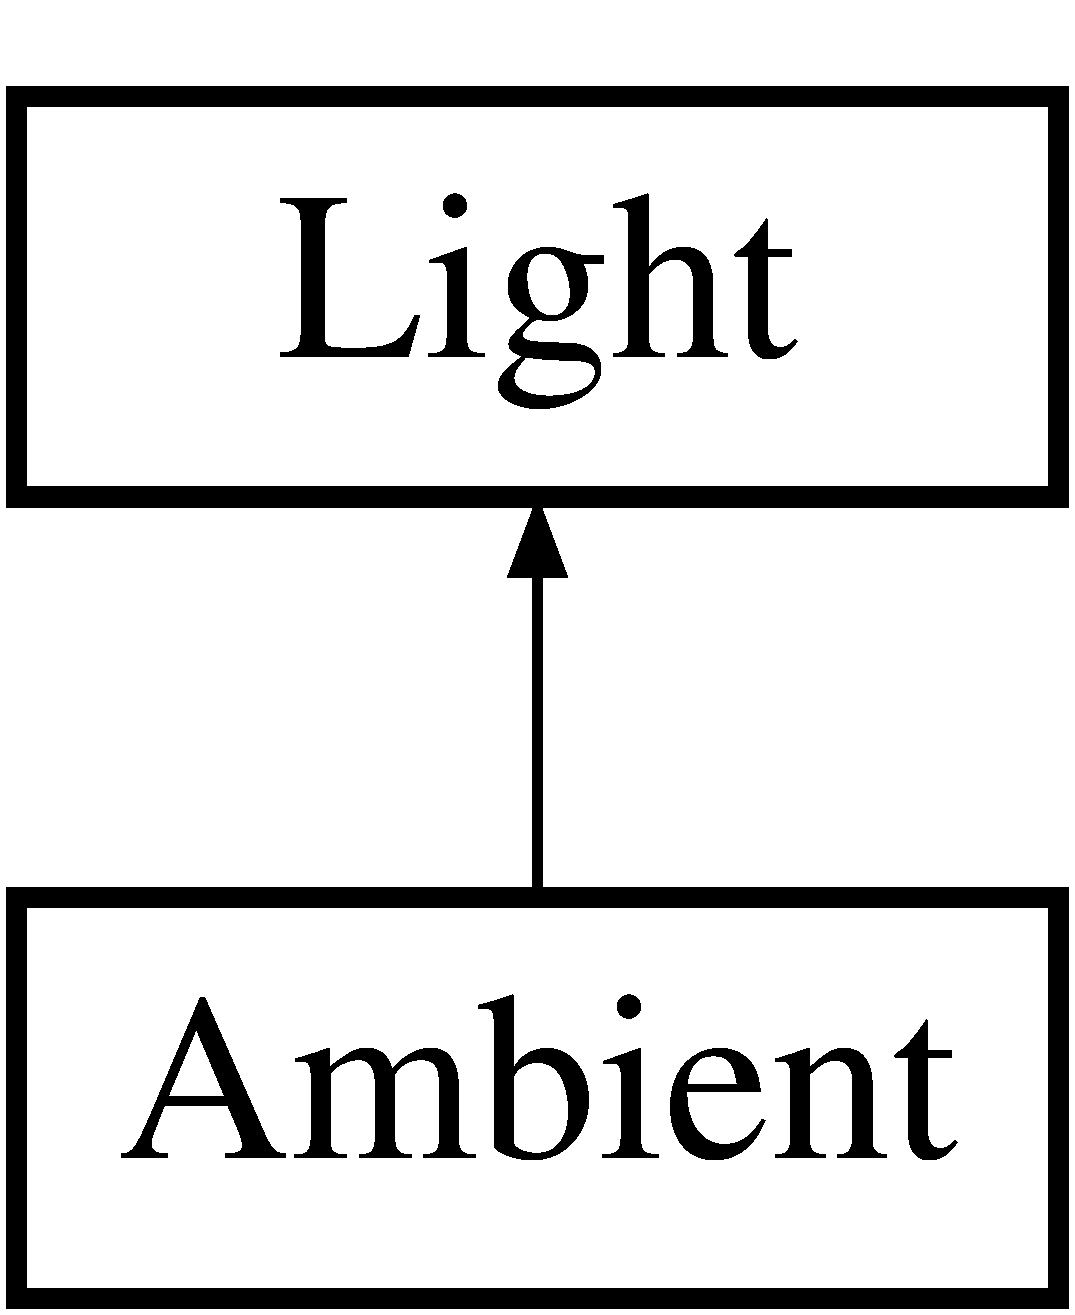
\includegraphics[height=2.000000cm]{class_ambient}
\end{center}
\end{figure}
\subsection*{Public Member Functions}
\begin{DoxyCompactItemize}
\item 
\hyperlink{class_ambient_a022e0d891287bc9bfc67a72e72a601d8}{Ambient} ()
\item 
virtual glm\+::vec3 \hyperlink{class_ambient_acb2fc1574883ea0bd41c662ec904164f}{Get\+Direction} (\hyperlink{class_surface}{Surface} \&sr)
\item 
virtual \hyperlink{class_r_g_b_color}{R\+G\+B\+Color} \hyperlink{class_ambient_aa75478ba2b30c9930ef538dd16f4586a}{L} (\hyperlink{class_surface}{Surface} \&sr)
\item 
virtual bool \hyperlink{class_ambient_a1373251f8db560b10061eb23f125bb27}{Shadowed} (const \hyperlink{class_ray}{Ray} \&ray, const \hyperlink{class_surface}{Surface} \&sr) const
\item 
void \hyperlink{group___lights_ga5aefcac18f63a3923320e634daff4f57}{Set\+Intensity} (const float intensity)
\item 
void \hyperlink{group___lights_gaac238172e351af4e5b302b0a006bf719}{Set\+Color} (const \hyperlink{class_r_g_b_color}{R\+G\+B\+Color} \&color)
\end{DoxyCompactItemize}
\subsection*{Additional Inherited Members}


\subsection{Detailed Description}
Representation of an ambient light source. \begin{DoxyRemark}{Remarks}
T\+O\+DO 
\end{DoxyRemark}


\subsection{Constructor \& Destructor Documentation}
\hypertarget{class_ambient_a022e0d891287bc9bfc67a72e72a601d8}{}\label{class_ambient_a022e0d891287bc9bfc67a72e72a601d8} 
\index{Ambient@{Ambient}!Ambient@{Ambient}}
\index{Ambient@{Ambient}!Ambient@{Ambient}}
\subsubsection{\texorpdfstring{Ambient()}{Ambient()}}
{\footnotesize\ttfamily Ambient\+::\+Ambient (\begin{DoxyParamCaption}{ }\end{DoxyParamCaption})}

Standard constructor. 

\subsection{Member Function Documentation}
\hypertarget{class_ambient_acb2fc1574883ea0bd41c662ec904164f}{}\label{class_ambient_acb2fc1574883ea0bd41c662ec904164f} 
\index{Ambient@{Ambient}!Get\+Direction@{Get\+Direction}}
\index{Get\+Direction@{Get\+Direction}!Ambient@{Ambient}}
\subsubsection{\texorpdfstring{Get\+Direction()}{GetDirection()}}
{\footnotesize\ttfamily virtual glm\+::vec3 Ambient\+::\+Get\+Direction (\begin{DoxyParamCaption}\item[{\hyperlink{class_surface}{Surface} \&}]{sr }\end{DoxyParamCaption})\hspace{0.3cm}{\ttfamily [virtual]}}

Computes the direction of the incoming light at a given surface. 
\begin{DoxyParams}{Parameters}
{\em sr} & Information about the surface of the object. \\
\hline
\end{DoxyParams}
\begin{DoxyReturn}{Returns}
Direction from which the light arrives at the surface. 
\end{DoxyReturn}


Implements \hyperlink{class_light_a62c5f73131ca1cdd6b2477f36c242482}{Light}.

\hypertarget{class_ambient_aa75478ba2b30c9930ef538dd16f4586a}{}\label{class_ambient_aa75478ba2b30c9930ef538dd16f4586a} 
\index{Ambient@{Ambient}!L@{L}}
\index{L@{L}!Ambient@{Ambient}}
\subsubsection{\texorpdfstring{L()}{L()}}
{\footnotesize\ttfamily virtual \hyperlink{class_r_g_b_color}{R\+G\+B\+Color} Ambient\+::L (\begin{DoxyParamCaption}\item[{\hyperlink{class_surface}{Surface} \&}]{sr }\end{DoxyParamCaption})\hspace{0.3cm}{\ttfamily [virtual]}}

Computes the incident radiance at a given surface. 
\begin{DoxyParams}{Parameters}
{\em sr} & Information about the surface of the object. \\
\hline
\end{DoxyParams}
\begin{DoxyReturn}{Returns}
Incident radiance at the surface. 
\end{DoxyReturn}


Reimplemented from \hyperlink{class_light_aba4ca1dcd52876cb5bee71ac8f684af5}{Light}.

\hypertarget{class_ambient_a1373251f8db560b10061eb23f125bb27}{}\label{class_ambient_a1373251f8db560b10061eb23f125bb27} 
\index{Ambient@{Ambient}!Shadowed@{Shadowed}}
\index{Shadowed@{Shadowed}!Ambient@{Ambient}}
\subsubsection{\texorpdfstring{Shadowed()}{Shadowed()}}
{\footnotesize\ttfamily virtual bool Ambient\+::\+Shadowed (\begin{DoxyParamCaption}\item[{const \hyperlink{class_ray}{Ray} \&}]{ray,  }\item[{const \hyperlink{class_surface}{Surface} \&}]{sr }\end{DoxyParamCaption}) const\hspace{0.3cm}{\ttfamily [virtual]}}

Checks if a surface is shadowed by another object. 
\begin{DoxyParams}{Parameters}
{\em ray} & Casted shadow ray. \\
\hline
{\em sr} & Information about the surface of the object. \\
\hline
\end{DoxyParams}
\begin{DoxyReturn}{Returns}
True, if the surface is shadowed. 
\end{DoxyReturn}


Implements \hyperlink{class_light_ac96c5efcdccb339609c7d19ea6ac5d17}{Light}.



The documentation for this class was generated from the following file\+:\begin{DoxyCompactItemize}
\item 
Source/\+Lights/include/\hyperlink{_ambient_8h}{Ambient.\+h}\end{DoxyCompactItemize}

\hypertarget{class_b_r_d_f}{}\section{B\+R\+DF Class Reference}
\label{class_b_r_d_f}\index{B\+R\+DF@{B\+R\+DF}}


{\ttfamily \#include $<$B\+R\+D\+F.\+h$>$}

Inheritance diagram for B\+R\+DF\+:\begin{figure}[H]
\begin{center}
\leavevmode
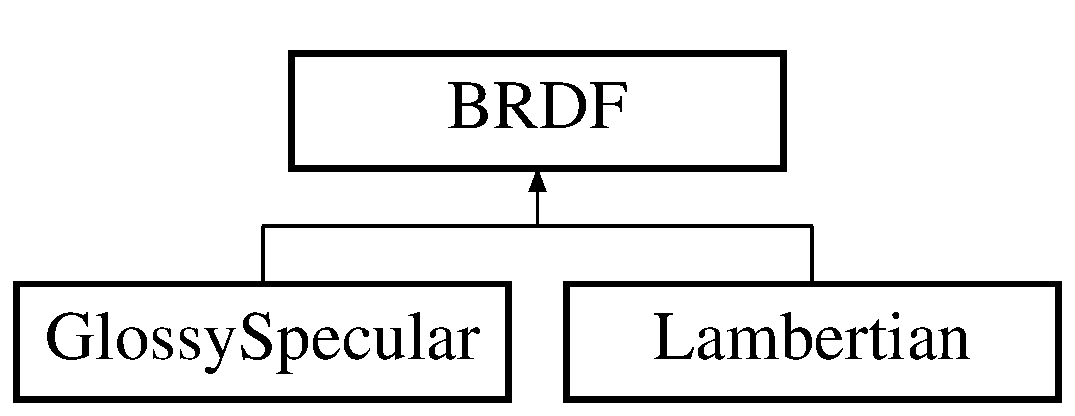
\includegraphics[height=2.000000cm]{class_b_r_d_f}
\end{center}
\end{figure}
\subsection*{Public Member Functions}
\begin{DoxyCompactItemize}
\item 
\hyperlink{class_b_r_d_f_a453d38b012c433272b117864f1902c52}{B\+R\+DF} ()
\item 
virtual \hyperlink{class_r_g_b_color}{R\+G\+B\+Color} \hyperlink{class_b_r_d_f_af3d87a4237b7b25b72ad1fb5027721bb}{f} (const \hyperlink{class_surface}{Surface} \&sr, const glm\+::vec3 \&wi, const glm\+::vec3 \&wo) const
\item 
virtual \hyperlink{class_r_g_b_color}{R\+G\+B\+Color} \hyperlink{class_b_r_d_f_a676438154e142c5762193ee5251e4d57}{rho} (const \hyperlink{class_surface}{Surface} \&sr, const glm\+::vec3 \&wo) const
\item 
virtual \hyperlink{class_r_g_b_color}{R\+G\+B\+Color} \hyperlink{class_b_r_d_f_a50d4e9c4729dc37a80e1948e6b7995d6}{SampleF} (\hyperlink{class_surface}{Surface} \&sr, const glm\+::vec3 \&wi, glm\+::vec3 \&wo)
\item 
virtual \hyperlink{class_r_g_b_color}{R\+G\+B\+Color} \hyperlink{class_b_r_d_f_a2abfe6323b1d0035439dbc2234ad2a34}{SampleF} (\hyperlink{class_surface}{Surface} \&sr, const glm\+::vec3 \&wi, glm\+::vec3 \&wo, float \&pdf)
\item 
void \hyperlink{group___b_r_d_f_ga77a2a5e48ca3093d853e5713afa01108}{Set\+Sampler} (std\+::shared\+\_\+ptr$<$ \hyperlink{class_sampler}{Sampler} $>$)
\end{DoxyCompactItemize}
\subsection*{Protected Attributes}
\begin{DoxyCompactItemize}
\item 
std\+::shared\+\_\+ptr$<$ \hyperlink{class_sampler}{Sampler} $>$ \hyperlink{class_b_r_d_f_a07f3aba126e7836a7cb86663428808f2}{m\+\_\+\+Sampler\+Ptr}
\end{DoxyCompactItemize}


\subsection{Detailed Description}
The bidirectional reflectance distribution function abstraction. \begin{DoxyRemark}{Remarks}
T\+O\+DO. 
\end{DoxyRemark}


\subsection{Constructor \& Destructor Documentation}
\hypertarget{class_b_r_d_f_a453d38b012c433272b117864f1902c52}{}\label{class_b_r_d_f_a453d38b012c433272b117864f1902c52} 
\index{B\+R\+DF@{B\+R\+DF}!B\+R\+DF@{B\+R\+DF}}
\index{B\+R\+DF@{B\+R\+DF}!B\+R\+DF@{B\+R\+DF}}
\subsubsection{\texorpdfstring{B\+R\+D\+F()}{BRDF()}}
{\footnotesize\ttfamily B\+R\+D\+F\+::\+B\+R\+DF (\begin{DoxyParamCaption}{ }\end{DoxyParamCaption})}

Standard constructor. 

\subsection{Member Function Documentation}
\hypertarget{class_b_r_d_f_af3d87a4237b7b25b72ad1fb5027721bb}{}\label{class_b_r_d_f_af3d87a4237b7b25b72ad1fb5027721bb} 
\index{B\+R\+DF@{B\+R\+DF}!f@{f}}
\index{f@{f}!B\+R\+DF@{B\+R\+DF}}
\subsubsection{\texorpdfstring{f()}{f()}}
{\footnotesize\ttfamily virtual \hyperlink{class_r_g_b_color}{R\+G\+B\+Color} B\+R\+D\+F\+::f (\begin{DoxyParamCaption}\item[{const \hyperlink{class_surface}{Surface} \&}]{sr,  }\item[{const glm\+::vec3 \&}]{wi,  }\item[{const glm\+::vec3 \&}]{wo }\end{DoxyParamCaption}) const\hspace{0.3cm}{\ttfamily [virtual]}}

Computes the reflected radiance along wo. 
\begin{DoxyParams}{Parameters}
{\em sr} & Information about the surface of the object. \\
\hline
{\em wi} & Incoming light direction. \\
\hline
{\em wo} & Reflected light direction. \\
\hline
\end{DoxyParams}
\begin{DoxyReturn}{Returns}
Reflected radiance of a surface. 
\end{DoxyReturn}


Reimplemented in \hyperlink{class_glossy_specular_a91b042f409462732c96eab041c2cc7c6}{Glossy\+Specular}, and \hyperlink{group___b_r_d_f_gad7b8c290aaacbe6c11ee62529dd7389b}{Lambertian}.

\hypertarget{class_b_r_d_f_a676438154e142c5762193ee5251e4d57}{}\label{class_b_r_d_f_a676438154e142c5762193ee5251e4d57} 
\index{B\+R\+DF@{B\+R\+DF}!rho@{rho}}
\index{rho@{rho}!B\+R\+DF@{B\+R\+DF}}
\subsubsection{\texorpdfstring{rho()}{rho()}}
{\footnotesize\ttfamily virtual \hyperlink{class_r_g_b_color}{R\+G\+B\+Color} B\+R\+D\+F\+::rho (\begin{DoxyParamCaption}\item[{const \hyperlink{class_surface}{Surface} \&}]{sr,  }\item[{const glm\+::vec3 \&}]{wo }\end{DoxyParamCaption}) const\hspace{0.3cm}{\ttfamily [virtual]}}

Computes the perfect diffuse reflectance. 
\begin{DoxyParams}{Parameters}
{\em sr} & Information about the surface of the object. \\
\hline
{\em wo} & Reflected light direction. \\
\hline
\end{DoxyParams}
\begin{DoxyReturn}{Returns}
Perfect diffuse reflectance. 
\end{DoxyReturn}


Reimplemented in \hyperlink{group___b_r_d_f_gaa70272886cbeb0f91c629ace938dd0a0}{Lambertian}.

\hypertarget{class_b_r_d_f_a50d4e9c4729dc37a80e1948e6b7995d6}{}\label{class_b_r_d_f_a50d4e9c4729dc37a80e1948e6b7995d6} 
\index{B\+R\+DF@{B\+R\+DF}!SampleF@{SampleF}}
\index{SampleF@{SampleF}!B\+R\+DF@{B\+R\+DF}}
\subsubsection{\texorpdfstring{Sample\+F()}{SampleF()}\hspace{0.1cm}{\footnotesize\ttfamily [1/2]}}
{\footnotesize\ttfamily virtual \hyperlink{class_r_g_b_color}{R\+G\+B\+Color} B\+R\+D\+F\+::\+SampleF (\begin{DoxyParamCaption}\item[{\hyperlink{class_surface}{Surface} \&}]{sr,  }\item[{const glm\+::vec3 \&}]{wi,  }\item[{glm\+::vec3 \&}]{wo }\end{DoxyParamCaption})\hspace{0.3cm}{\ttfamily [virtual]}}

T\+O\+DO. 
\begin{DoxyParams}{Parameters}
{\em sr} & Information about the surface of the object. \\
\hline
{\em wi} & Incoming light direction. \\
\hline
{\em wo} & Reflected light direction. \\
\hline
\end{DoxyParams}
\begin{DoxyReturn}{Returns}

\end{DoxyReturn}
\hypertarget{class_b_r_d_f_a2abfe6323b1d0035439dbc2234ad2a34}{}\label{class_b_r_d_f_a2abfe6323b1d0035439dbc2234ad2a34} 
\index{B\+R\+DF@{B\+R\+DF}!SampleF@{SampleF}}
\index{SampleF@{SampleF}!B\+R\+DF@{B\+R\+DF}}
\subsubsection{\texorpdfstring{Sample\+F()}{SampleF()}\hspace{0.1cm}{\footnotesize\ttfamily [2/2]}}
{\footnotesize\ttfamily virtual \hyperlink{class_r_g_b_color}{R\+G\+B\+Color} B\+R\+D\+F\+::\+SampleF (\begin{DoxyParamCaption}\item[{\hyperlink{class_surface}{Surface} \&}]{sr,  }\item[{const glm\+::vec3 \&}]{wi,  }\item[{glm\+::vec3 \&}]{wo,  }\item[{float \&}]{pdf }\end{DoxyParamCaption})\hspace{0.3cm}{\ttfamily [virtual]}}

T\+O\+DO 
\begin{DoxyParams}{Parameters}
{\em sr} & Information about the surface of the object. \\
\hline
{\em wi} & Incoming light direction. \\
\hline
{\em wo} & Reflected light direction. \\
\hline
{\em pdf} & Probability density function. \\
\hline
\end{DoxyParams}
\begin{DoxyReturn}{Returns}

\end{DoxyReturn}


\subsection{Member Data Documentation}
\hypertarget{class_b_r_d_f_a07f3aba126e7836a7cb86663428808f2}{}\label{class_b_r_d_f_a07f3aba126e7836a7cb86663428808f2} 
\index{B\+R\+DF@{B\+R\+DF}!m\+\_\+\+Sampler\+Ptr@{m\+\_\+\+Sampler\+Ptr}}
\index{m\+\_\+\+Sampler\+Ptr@{m\+\_\+\+Sampler\+Ptr}!B\+R\+DF@{B\+R\+DF}}
\subsubsection{\texorpdfstring{m\+\_\+\+Sampler\+Ptr}{m\_SamplerPtr}}
{\footnotesize\ttfamily std\+::shared\+\_\+ptr$<$\hyperlink{class_sampler}{Sampler}$>$ B\+R\+D\+F\+::m\+\_\+\+Sampler\+Ptr\hspace{0.3cm}{\ttfamily [protected]}}

Pointer to the sampler attached to the \hyperlink{class_b_r_d_f}{B\+R\+DF} object. 

The documentation for this class was generated from the following file\+:\begin{DoxyCompactItemize}
\item 
Source/\+B\+R\+D\+Fs/include/\hyperlink{_b_r_d_f_8h}{B\+R\+D\+F.\+h}\end{DoxyCompactItemize}

\hypertarget{class_camera}{}\section{Camera Class Reference}
\label{class_camera}\index{Camera@{Camera}}


{\ttfamily \#include $<$Camera.\+h$>$}

Inheritance diagram for Camera\+:\begin{figure}[H]
\begin{center}
\leavevmode
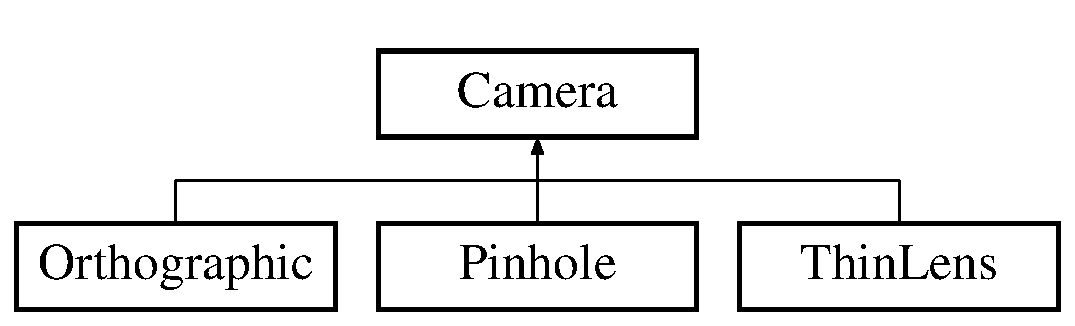
\includegraphics[height=2.000000cm]{class_camera}
\end{center}
\end{figure}
\subsection*{Public Member Functions}
\begin{DoxyCompactItemize}
\item 
\hyperlink{class_camera_a01f94c3543f56ede7af49dc778f19331}{Camera} ()
\item 
virtual void \hyperlink{class_camera_ad65367e9b225387219d013ffed3f621a}{Render\+Scene} (const World \&w)=0
\item 
void \hyperlink{group___cameras_gad2265245e85699e077dc1d8d33eecece}{Set\+Eye} (const glm\+::vec3 \&eye)
\item 
void \hyperlink{group___cameras_ga92295d79a45f2ab1756221836567997a}{Look\+At} (const glm\+::vec3 \&look\+\_\+at)
\item 
void \hyperlink{group___cameras_gaa6c9c847b6db5c4d6450fb9b75f26e81}{Set\+Up\+Vector} (const glm\+::vec3 \&up)
\item 
void \hyperlink{group___cameras_ga0e499019f7cd3029602461fcd63aa40c}{Set\+Yaw} (const float yaw)
\item 
void \hyperlink{group___cameras_ga33e125b9d164e7332dba4cc01c468d6c}{Set\+Pitch} (const float pitch)
\item 
void \hyperlink{group___cameras_ga2c07ac7e812f4dab134fc06692fcaf11}{Set\+Roll} (const float roll)
\item 
void \hyperlink{group___cameras_gaf9985918fc0135ac8c98344c96129509}{Set\+Exposure\+Time} (const float etime)
\end{DoxyCompactItemize}
\subsection*{Protected Member Functions}
\begin{DoxyCompactItemize}
\item 
void \hyperlink{class_camera_ab2a27d88b13f4cab92d62bc421650e7b}{Compute\+U\+VW} ()
\end{DoxyCompactItemize}
\subsection*{Protected Attributes}
\begin{DoxyCompactItemize}
\item 
glm\+::vec3 \hyperlink{class_camera_afea4cf59abeabef0ac61915bccd1c35c}{m\+\_\+\+Eye}
\item 
glm\+::vec3 \hyperlink{class_camera_a64c0c57201219d5e9965298a19007a61}{m\+\_\+\+Look\+At}
\item 
glm\+::vec3 \hyperlink{class_camera_ae48ab25a4c2c9a91e6814db0c1abe72c}{m\+\_\+\+Up\+Vector}
\item 
glm\+::vec3 \hyperlink{class_camera_a544f5de8d6c0b2d9aea1a9cff9f0aeb6}{m\+\_\+U}
\item 
glm\+::vec3 \hyperlink{class_camera_a2bfb4e67db9d92f152913c8cb8159797}{m\+\_\+V}
\item 
glm\+::vec3 \hyperlink{class_camera_a75de71e6e4b12d69d46d84d04f37c7c3}{m\+\_\+W}
\item 
float \hyperlink{class_camera_ac3b7d101ef808536cac0f679deef5f9c}{m\+\_\+\+Yaw}
\item 
float \hyperlink{class_camera_aac745762c9d82b5cdfdcd48c7902b919}{m\+\_\+\+Pitch}
\item 
float \hyperlink{class_camera_a58eab74ebcfe6a72ae0d6df32a102181}{m\+\_\+\+Roll}
\item 
float \hyperlink{class_camera_a9930c812c2015bf0f3746c18ff2d3e3b}{m\+\_\+\+Exposure\+Time}
\end{DoxyCompactItemize}


\subsection{Detailed Description}
A point from which the scene will be rendered. \begin{DoxyRemark}{Remarks}
T\+O\+DO. 
\end{DoxyRemark}


\subsection{Constructor \& Destructor Documentation}
\hypertarget{class_camera_a01f94c3543f56ede7af49dc778f19331}{}\label{class_camera_a01f94c3543f56ede7af49dc778f19331} 
\index{Camera@{Camera}!Camera@{Camera}}
\index{Camera@{Camera}!Camera@{Camera}}
\subsubsection{\texorpdfstring{Camera()}{Camera()}}
{\footnotesize\ttfamily Camera\+::\+Camera (\begin{DoxyParamCaption}{ }\end{DoxyParamCaption})}

Standard constructor. 

\subsection{Member Function Documentation}
\hypertarget{class_camera_ab2a27d88b13f4cab92d62bc421650e7b}{}\label{class_camera_ab2a27d88b13f4cab92d62bc421650e7b} 
\index{Camera@{Camera}!Compute\+U\+VW@{Compute\+U\+VW}}
\index{Compute\+U\+VW@{Compute\+U\+VW}!Camera@{Camera}}
\subsubsection{\texorpdfstring{Compute\+U\+V\+W()}{ComputeUVW()}}
{\footnotesize\ttfamily void Camera\+::\+Compute\+U\+VW (\begin{DoxyParamCaption}{ }\end{DoxyParamCaption})\hspace{0.3cm}{\ttfamily [protected]}}

Computes the orthonormal basis of the camera. \hypertarget{class_camera_ad65367e9b225387219d013ffed3f621a}{}\label{class_camera_ad65367e9b225387219d013ffed3f621a} 
\index{Camera@{Camera}!Render\+Scene@{Render\+Scene}}
\index{Render\+Scene@{Render\+Scene}!Camera@{Camera}}
\subsubsection{\texorpdfstring{Render\+Scene()}{RenderScene()}}
{\footnotesize\ttfamily virtual void Camera\+::\+Render\+Scene (\begin{DoxyParamCaption}\item[{const World \&}]{w }\end{DoxyParamCaption})\hspace{0.3cm}{\ttfamily [pure virtual]}}

Traces the constructed scene. 
\begin{DoxyParams}{Parameters}
{\em w} & Reference to the world. \\
\hline
\end{DoxyParams}


Implemented in \hyperlink{class_orthographic_a0d7ee7bfe619febed73725b99d2cc0b0}{Orthographic}, \hyperlink{class_pinhole_a722af80f738cf4e8adba65926ffea9c9}{Pinhole}, and \hyperlink{class_thin_lens_af33d499e8fdbdbd196ba3a9b28bdaf5c}{Thin\+Lens}.



\subsection{Member Data Documentation}
\hypertarget{class_camera_a9930c812c2015bf0f3746c18ff2d3e3b}{}\label{class_camera_a9930c812c2015bf0f3746c18ff2d3e3b} 
\index{Camera@{Camera}!m\+\_\+\+Exposure\+Time@{m\+\_\+\+Exposure\+Time}}
\index{m\+\_\+\+Exposure\+Time@{m\+\_\+\+Exposure\+Time}!Camera@{Camera}}
\subsubsection{\texorpdfstring{m\+\_\+\+Exposure\+Time}{m\_ExposureTime}}
{\footnotesize\ttfamily float Camera\+::m\+\_\+\+Exposure\+Time\hspace{0.3cm}{\ttfamily [protected]}}

Exposure time of the camera. \hypertarget{class_camera_afea4cf59abeabef0ac61915bccd1c35c}{}\label{class_camera_afea4cf59abeabef0ac61915bccd1c35c} 
\index{Camera@{Camera}!m\+\_\+\+Eye@{m\+\_\+\+Eye}}
\index{m\+\_\+\+Eye@{m\+\_\+\+Eye}!Camera@{Camera}}
\subsubsection{\texorpdfstring{m\+\_\+\+Eye}{m\_Eye}}
{\footnotesize\ttfamily glm\+::vec3 Camera\+::m\+\_\+\+Eye\hspace{0.3cm}{\ttfamily [protected]}}

Eye position in world coordinates. \hypertarget{class_camera_a64c0c57201219d5e9965298a19007a61}{}\label{class_camera_a64c0c57201219d5e9965298a19007a61} 
\index{Camera@{Camera}!m\+\_\+\+Look\+At@{m\+\_\+\+Look\+At}}
\index{m\+\_\+\+Look\+At@{m\+\_\+\+Look\+At}!Camera@{Camera}}
\subsubsection{\texorpdfstring{m\+\_\+\+Look\+At}{m\_LookAt}}
{\footnotesize\ttfamily glm\+::vec3 Camera\+::m\+\_\+\+Look\+At\hspace{0.3cm}{\ttfamily [protected]}}

Direction the camera is facing. \hypertarget{class_camera_aac745762c9d82b5cdfdcd48c7902b919}{}\label{class_camera_aac745762c9d82b5cdfdcd48c7902b919} 
\index{Camera@{Camera}!m\+\_\+\+Pitch@{m\+\_\+\+Pitch}}
\index{m\+\_\+\+Pitch@{m\+\_\+\+Pitch}!Camera@{Camera}}
\subsubsection{\texorpdfstring{m\+\_\+\+Pitch}{m\_Pitch}}
{\footnotesize\ttfamily float Camera\+::m\+\_\+\+Pitch\hspace{0.3cm}{\ttfamily [protected]}}

Pitch angle of the camera. \hypertarget{class_camera_a58eab74ebcfe6a72ae0d6df32a102181}{}\label{class_camera_a58eab74ebcfe6a72ae0d6df32a102181} 
\index{Camera@{Camera}!m\+\_\+\+Roll@{m\+\_\+\+Roll}}
\index{m\+\_\+\+Roll@{m\+\_\+\+Roll}!Camera@{Camera}}
\subsubsection{\texorpdfstring{m\+\_\+\+Roll}{m\_Roll}}
{\footnotesize\ttfamily float Camera\+::m\+\_\+\+Roll\hspace{0.3cm}{\ttfamily [protected]}}

Roll angle of the camera. \hypertarget{class_camera_a544f5de8d6c0b2d9aea1a9cff9f0aeb6}{}\label{class_camera_a544f5de8d6c0b2d9aea1a9cff9f0aeb6} 
\index{Camera@{Camera}!m\+\_\+U@{m\+\_\+U}}
\index{m\+\_\+U@{m\+\_\+U}!Camera@{Camera}}
\subsubsection{\texorpdfstring{m\+\_\+U}{m\_U}}
{\footnotesize\ttfamily glm\+::vec3 Camera\+::m\+\_\+U\hspace{0.3cm}{\ttfamily [protected]}}

X vector of the camera in its coordinate system. \hypertarget{class_camera_ae48ab25a4c2c9a91e6814db0c1abe72c}{}\label{class_camera_ae48ab25a4c2c9a91e6814db0c1abe72c} 
\index{Camera@{Camera}!m\+\_\+\+Up\+Vector@{m\+\_\+\+Up\+Vector}}
\index{m\+\_\+\+Up\+Vector@{m\+\_\+\+Up\+Vector}!Camera@{Camera}}
\subsubsection{\texorpdfstring{m\+\_\+\+Up\+Vector}{m\_UpVector}}
{\footnotesize\ttfamily glm\+::vec3 Camera\+::m\+\_\+\+Up\+Vector\hspace{0.3cm}{\ttfamily [protected]}}

World\textquotesingle{}s up vector. \hypertarget{class_camera_a2bfb4e67db9d92f152913c8cb8159797}{}\label{class_camera_a2bfb4e67db9d92f152913c8cb8159797} 
\index{Camera@{Camera}!m\+\_\+V@{m\+\_\+V}}
\index{m\+\_\+V@{m\+\_\+V}!Camera@{Camera}}
\subsubsection{\texorpdfstring{m\+\_\+V}{m\_V}}
{\footnotesize\ttfamily glm\+::vec3 Camera\+::m\+\_\+V\hspace{0.3cm}{\ttfamily [protected]}}

Y vector of the camera in its coordinate system. \hypertarget{class_camera_a75de71e6e4b12d69d46d84d04f37c7c3}{}\label{class_camera_a75de71e6e4b12d69d46d84d04f37c7c3} 
\index{Camera@{Camera}!m\+\_\+W@{m\+\_\+W}}
\index{m\+\_\+W@{m\+\_\+W}!Camera@{Camera}}
\subsubsection{\texorpdfstring{m\+\_\+W}{m\_W}}
{\footnotesize\ttfamily glm\+::vec3 Camera\+::m\+\_\+W\hspace{0.3cm}{\ttfamily [protected]}}

Z vector of the camera in its coordinate system. \hypertarget{class_camera_ac3b7d101ef808536cac0f679deef5f9c}{}\label{class_camera_ac3b7d101ef808536cac0f679deef5f9c} 
\index{Camera@{Camera}!m\+\_\+\+Yaw@{m\+\_\+\+Yaw}}
\index{m\+\_\+\+Yaw@{m\+\_\+\+Yaw}!Camera@{Camera}}
\subsubsection{\texorpdfstring{m\+\_\+\+Yaw}{m\_Yaw}}
{\footnotesize\ttfamily float Camera\+::m\+\_\+\+Yaw\hspace{0.3cm}{\ttfamily [protected]}}

Yaw angle of the camera. 

The documentation for this class was generated from the following file\+:\begin{DoxyCompactItemize}
\item 
Source/\+Cameras/include/\hyperlink{_camera_8h}{Camera.\+h}\end{DoxyCompactItemize}

\hypertarget{class_directional}{}\section{Directional Class Reference}
\label{class_directional}\index{Directional@{Directional}}


{\ttfamily \#include $<$Directional.\+h$>$}

Inheritance diagram for Directional\+:\begin{figure}[H]
\begin{center}
\leavevmode
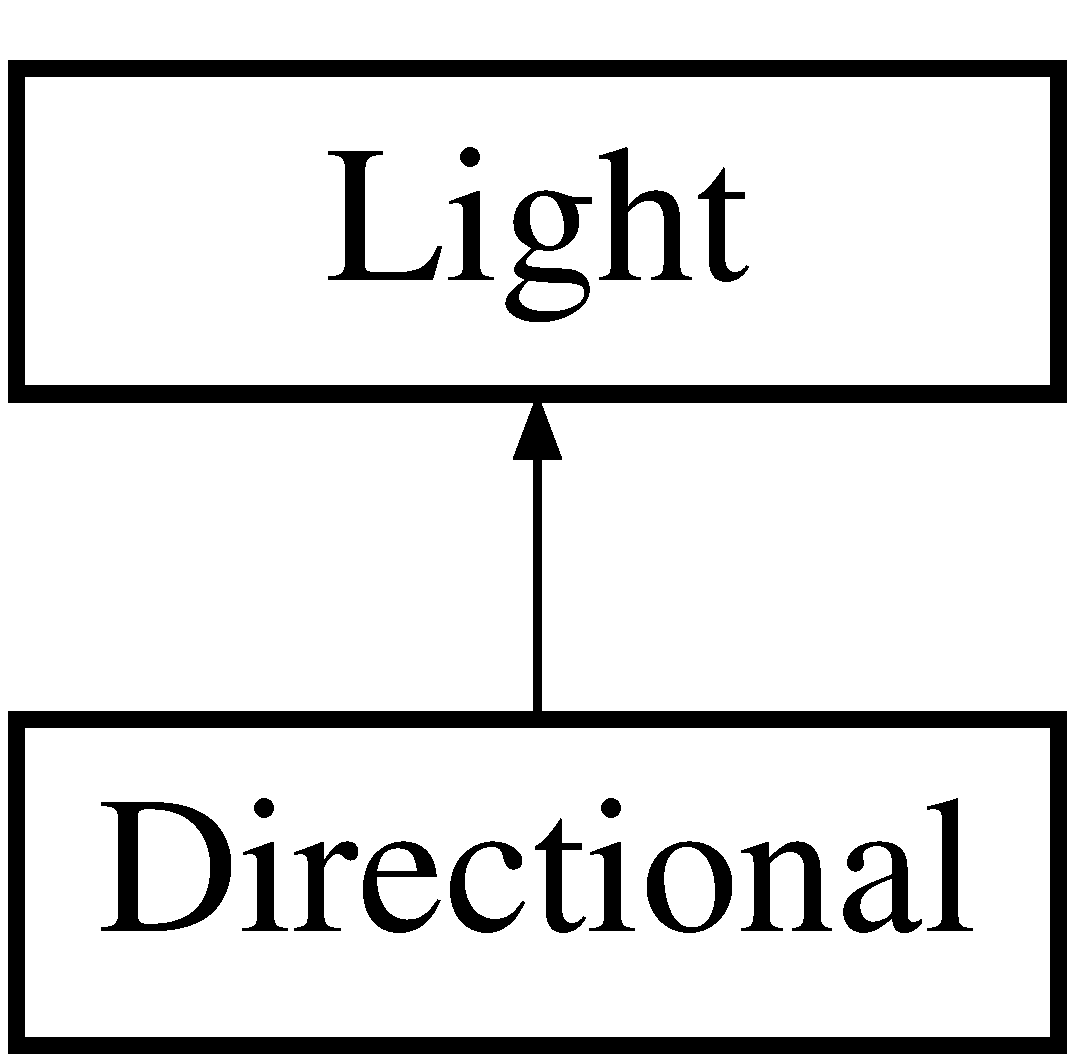
\includegraphics[height=2.000000cm]{class_directional}
\end{center}
\end{figure}
\subsection*{Public Member Functions}
\begin{DoxyCompactItemize}
\item 
\hyperlink{class_directional_a3e88e0e393dbb8e57dbb7218c5d9f8c1}{Directional} ()
\item 
virtual glm\+::vec3 \hyperlink{class_directional_a022fc1cb35f0f760b5472c06ad6e2e74}{Get\+Direction} (\hyperlink{class_surface}{Surface} \&sr)
\item 
virtual \hyperlink{class_r_g_b_color}{R\+G\+B\+Color} \hyperlink{class_directional_ac9a728a89d32c5f62ddef2be6c3e467d}{L} (\hyperlink{class_surface}{Surface} \&sr)
\item 
virtual bool \hyperlink{class_directional_a56a42abcdb41df1e3dd44b173aee494a}{Shadowed} (const \hyperlink{class_ray}{Ray} \&ray, const \hyperlink{class_surface}{Surface} \&sr) const
\item 
void \hyperlink{group___lights_gaa916930bad1e02ef24f89039151be8cd}{Set\+Intensity} (const float intensity)
\item 
void \hyperlink{group___lights_ga460c4d38eba389fd8e13d994249bbafc}{Set\+Color} (const \hyperlink{class_r_g_b_color}{R\+G\+B\+Color} \&color)
\item 
void \hyperlink{group___lights_ga497358d0a37e4a87d5e24f286695c0a6}{Set\+Direction} (const glm\+::vec3 \&direction)
\end{DoxyCompactItemize}
\subsection*{Additional Inherited Members}


\subsection{Detailed Description}
Representation of a directional light source. \begin{DoxyRemark}{Remarks}
T\+O\+DO 
\end{DoxyRemark}


\subsection{Constructor \& Destructor Documentation}
\hypertarget{class_directional_a3e88e0e393dbb8e57dbb7218c5d9f8c1}{}\label{class_directional_a3e88e0e393dbb8e57dbb7218c5d9f8c1} 
\index{Directional@{Directional}!Directional@{Directional}}
\index{Directional@{Directional}!Directional@{Directional}}
\subsubsection{\texorpdfstring{Directional()}{Directional()}}
{\footnotesize\ttfamily Directional\+::\+Directional (\begin{DoxyParamCaption}{ }\end{DoxyParamCaption})}

Standard constructor. 

\subsection{Member Function Documentation}
\hypertarget{class_directional_a022fc1cb35f0f760b5472c06ad6e2e74}{}\label{class_directional_a022fc1cb35f0f760b5472c06ad6e2e74} 
\index{Directional@{Directional}!Get\+Direction@{Get\+Direction}}
\index{Get\+Direction@{Get\+Direction}!Directional@{Directional}}
\subsubsection{\texorpdfstring{Get\+Direction()}{GetDirection()}}
{\footnotesize\ttfamily virtual glm\+::vec3 Directional\+::\+Get\+Direction (\begin{DoxyParamCaption}\item[{\hyperlink{class_surface}{Surface} \&}]{sr }\end{DoxyParamCaption})\hspace{0.3cm}{\ttfamily [virtual]}}

Computes the direction of the incoming light at a given surface. 
\begin{DoxyParams}{Parameters}
{\em sr} & Information about the surface of the object. \\
\hline
\end{DoxyParams}
\begin{DoxyReturn}{Returns}
Direction from which the light arrives at the surface. 
\end{DoxyReturn}


Implements \hyperlink{class_light_a62c5f73131ca1cdd6b2477f36c242482}{Light}.

\hypertarget{class_directional_ac9a728a89d32c5f62ddef2be6c3e467d}{}\label{class_directional_ac9a728a89d32c5f62ddef2be6c3e467d} 
\index{Directional@{Directional}!L@{L}}
\index{L@{L}!Directional@{Directional}}
\subsubsection{\texorpdfstring{L()}{L()}}
{\footnotesize\ttfamily virtual \hyperlink{class_r_g_b_color}{R\+G\+B\+Color} Directional\+::L (\begin{DoxyParamCaption}\item[{\hyperlink{class_surface}{Surface} \&}]{sr }\end{DoxyParamCaption})\hspace{0.3cm}{\ttfamily [virtual]}}

Computes the incident radiance at a given surface. 
\begin{DoxyParams}{Parameters}
{\em sr} & Information about the surface of the object. \\
\hline
\end{DoxyParams}
\begin{DoxyReturn}{Returns}
Incident radiance at the surface. 
\end{DoxyReturn}


Reimplemented from \hyperlink{class_light_aba4ca1dcd52876cb5bee71ac8f684af5}{Light}.

\hypertarget{class_directional_a56a42abcdb41df1e3dd44b173aee494a}{}\label{class_directional_a56a42abcdb41df1e3dd44b173aee494a} 
\index{Directional@{Directional}!Shadowed@{Shadowed}}
\index{Shadowed@{Shadowed}!Directional@{Directional}}
\subsubsection{\texorpdfstring{Shadowed()}{Shadowed()}}
{\footnotesize\ttfamily virtual bool Directional\+::\+Shadowed (\begin{DoxyParamCaption}\item[{const \hyperlink{class_ray}{Ray} \&}]{ray,  }\item[{const \hyperlink{class_surface}{Surface} \&}]{sr }\end{DoxyParamCaption}) const\hspace{0.3cm}{\ttfamily [virtual]}}

Checks if a surface is shadowed by another object. 
\begin{DoxyParams}{Parameters}
{\em ray} & Casted shadow ray. \\
\hline
{\em sr} & Information about the surface of the object. \\
\hline
\end{DoxyParams}
\begin{DoxyReturn}{Returns}
True, if the surface is shadowed. 
\end{DoxyReturn}


Implements \hyperlink{class_light_ac96c5efcdccb339609c7d19ea6ac5d17}{Light}.



The documentation for this class was generated from the following file\+:\begin{DoxyCompactItemize}
\item 
Source/\+Lights/include/\hyperlink{_directional_8h}{Directional.\+h}\end{DoxyCompactItemize}

\hypertarget{class_glossy_specular}{}\section{Glossy\+Specular Class Reference}
\label{class_glossy_specular}\index{Glossy\+Specular@{Glossy\+Specular}}


{\ttfamily \#include $<$Glossy\+Specular.\+h$>$}

Inheritance diagram for Glossy\+Specular\+:\begin{figure}[H]
\begin{center}
\leavevmode
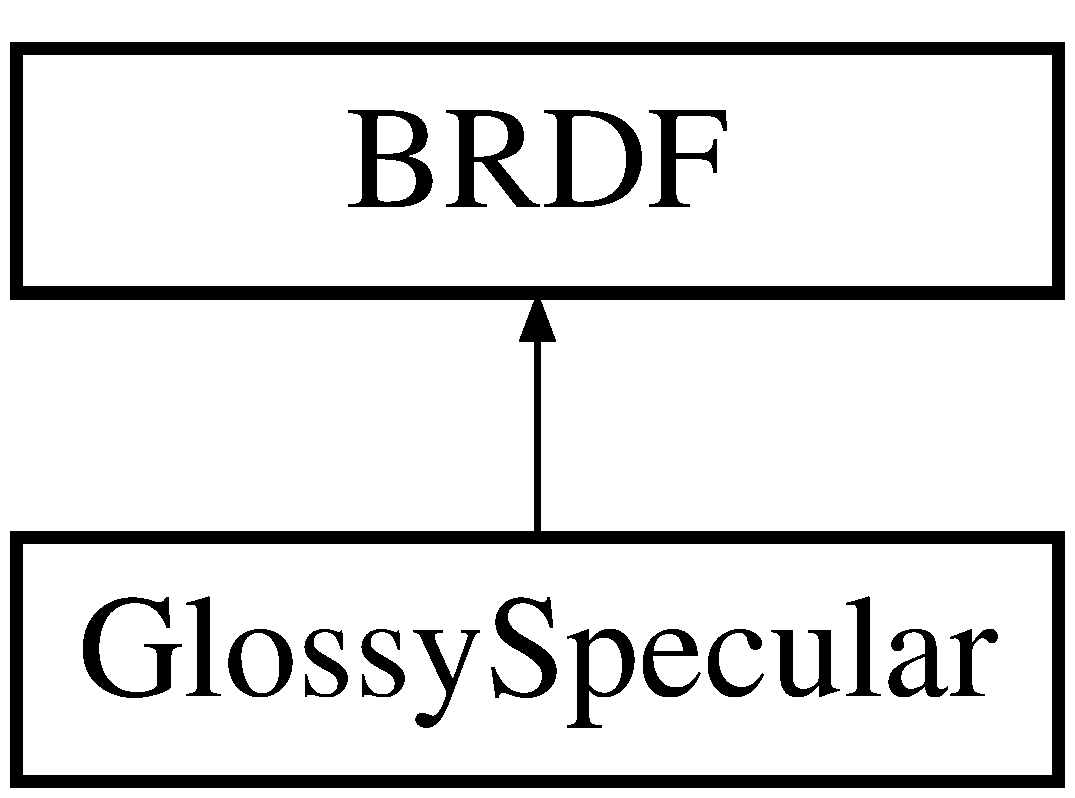
\includegraphics[height=2.000000cm]{class_glossy_specular}
\end{center}
\end{figure}
\subsection*{Public Member Functions}
\begin{DoxyCompactItemize}
\item 
\hyperlink{class_glossy_specular_ae6e09109ef43e05bab37fc3086115787}{Glossy\+Specular} ()
\item 
virtual \hyperlink{class_r_g_b_color}{R\+G\+B\+Color} \hyperlink{class_glossy_specular_a91b042f409462732c96eab041c2cc7c6}{f} (const \hyperlink{class_surface}{Surface} \&sr, const glm\+::vec3 \&wi, const glm\+::vec3 \&wo) const
\item 
void \hyperlink{group___b_r_d_f_gab7e40f362680b631c40530c9c605e3b3}{Set\+Specular\+Reflection} (const float ksr)
\item 
void \hyperlink{group___b_r_d_f_ga4bc78448419beb3d49ae4a9d96a8c5ad}{Set\+Specular\+Color} (const \hyperlink{class_r_g_b_color}{R\+G\+B\+Color} \&color)
\item 
void \hyperlink{group___b_r_d_f_ga06b9d29c576be7fcacef68edb57cfc23}{Set\+Specular\+Exponent} (const float ksexp)
\end{DoxyCompactItemize}
\subsection*{Additional Inherited Members}


\subsection{Detailed Description}
The glossy specular bidirectional reflectance distribution function abstraction. \begin{DoxyRemark}{Remarks}
T\+O\+DO. 
\end{DoxyRemark}


\subsection{Constructor \& Destructor Documentation}
\hypertarget{class_glossy_specular_ae6e09109ef43e05bab37fc3086115787}{}\label{class_glossy_specular_ae6e09109ef43e05bab37fc3086115787} 
\index{Glossy\+Specular@{Glossy\+Specular}!Glossy\+Specular@{Glossy\+Specular}}
\index{Glossy\+Specular@{Glossy\+Specular}!Glossy\+Specular@{Glossy\+Specular}}
\subsubsection{\texorpdfstring{Glossy\+Specular()}{GlossySpecular()}}
{\footnotesize\ttfamily Glossy\+Specular\+::\+Glossy\+Specular (\begin{DoxyParamCaption}{ }\end{DoxyParamCaption})}

Standard constructor. 

\subsection{Member Function Documentation}
\hypertarget{class_glossy_specular_a91b042f409462732c96eab041c2cc7c6}{}\label{class_glossy_specular_a91b042f409462732c96eab041c2cc7c6} 
\index{Glossy\+Specular@{Glossy\+Specular}!f@{f}}
\index{f@{f}!Glossy\+Specular@{Glossy\+Specular}}
\subsubsection{\texorpdfstring{f()}{f()}}
{\footnotesize\ttfamily virtual \hyperlink{class_r_g_b_color}{R\+G\+B\+Color} Glossy\+Specular\+::f (\begin{DoxyParamCaption}\item[{const \hyperlink{class_surface}{Surface} \&}]{sr,  }\item[{const glm\+::vec3 \&}]{wi,  }\item[{const glm\+::vec3 \&}]{wo }\end{DoxyParamCaption}) const\hspace{0.3cm}{\ttfamily [virtual]}}

Computes the reflected radiance along wo. 
\begin{DoxyParams}{Parameters}
{\em sr} & Information about the surface of the object. \\
\hline
{\em wi} & Incoming light direction. \\
\hline
{\em wo} & Reflected light direction. \\
\hline
\end{DoxyParams}
\begin{DoxyReturn}{Returns}
Reflected radiance of a surface. 
\end{DoxyReturn}


Reimplemented from \hyperlink{class_b_r_d_f_af3d87a4237b7b25b72ad1fb5027721bb}{B\+R\+DF}.



The documentation for this class was generated from the following file\+:\begin{DoxyCompactItemize}
\item 
Source/\+B\+R\+D\+Fs/include/\hyperlink{_glossy_specular_8h}{Glossy\+Specular.\+h}\end{DoxyCompactItemize}

\hypertarget{class_hammersley}{}\section{Hammersley Class Reference}
\label{class_hammersley}\index{Hammersley@{Hammersley}}


{\ttfamily \#include $<$Hammersley.\+h$>$}

Inheritance diagram for Hammersley\+:\begin{figure}[H]
\begin{center}
\leavevmode
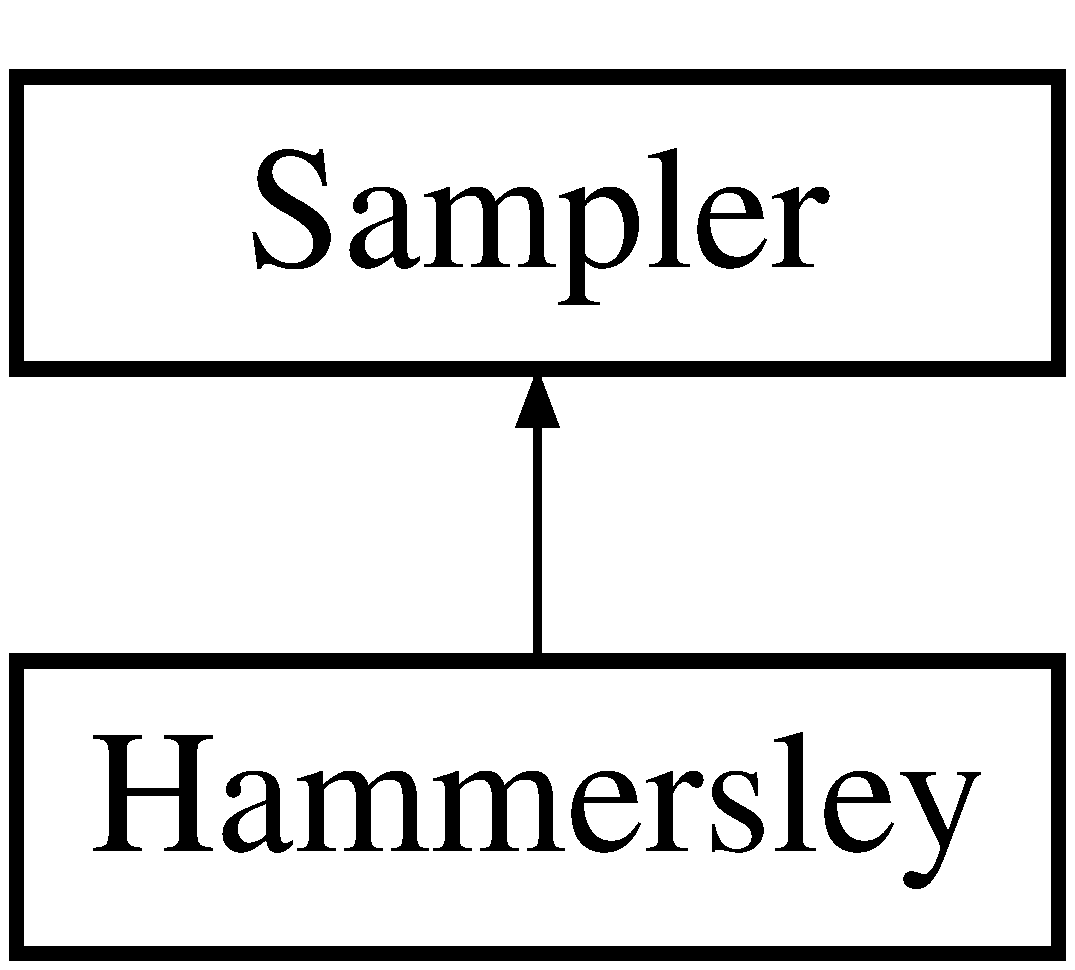
\includegraphics[height=2.000000cm]{class_hammersley}
\end{center}
\end{figure}
\subsection*{Public Member Functions}
\begin{DoxyCompactItemize}
\item 
\hyperlink{class_hammersley_a326c4955c1013974aff591c9425c9be7}{Hammersley} ()
\item 
\hyperlink{class_hammersley_afeef5879129f035ef70c87cecce7aaa9}{Hammersley} (const int num\+Samples)
\item 
\hyperlink{class_hammersley_a7e59d7d7df2709d1ccf3beedfb3da33b}{Hammersley} (const int num\+Samples, const int num\+Sets)
\end{DoxyCompactItemize}
\subsection*{Additional Inherited Members}


\subsection{Detailed Description}
T\+O\+DO \begin{DoxyRemark}{Remarks}
T\+O\+DO. 
\end{DoxyRemark}


\subsection{Constructor \& Destructor Documentation}
\hypertarget{class_hammersley_a326c4955c1013974aff591c9425c9be7}{}\label{class_hammersley_a326c4955c1013974aff591c9425c9be7} 
\index{Hammersley@{Hammersley}!Hammersley@{Hammersley}}
\index{Hammersley@{Hammersley}!Hammersley@{Hammersley}}
\subsubsection{\texorpdfstring{Hammersley()}{Hammersley()}\hspace{0.1cm}{\footnotesize\ttfamily [1/3]}}
{\footnotesize\ttfamily Hammersley\+::\+Hammersley (\begin{DoxyParamCaption}{ }\end{DoxyParamCaption})}

Standard constructor. \hypertarget{class_hammersley_afeef5879129f035ef70c87cecce7aaa9}{}\label{class_hammersley_afeef5879129f035ef70c87cecce7aaa9} 
\index{Hammersley@{Hammersley}!Hammersley@{Hammersley}}
\index{Hammersley@{Hammersley}!Hammersley@{Hammersley}}
\subsubsection{\texorpdfstring{Hammersley()}{Hammersley()}\hspace{0.1cm}{\footnotesize\ttfamily [2/3]}}
{\footnotesize\ttfamily Hammersley\+::\+Hammersley (\begin{DoxyParamCaption}\item[{const int}]{num\+Samples }\end{DoxyParamCaption})}

Constructs a sampler and sets its number of samples. 
\begin{DoxyParams}{Parameters}
{\em num\+Samples} & Number of samples. \\
\hline
\end{DoxyParams}
\hypertarget{class_hammersley_a7e59d7d7df2709d1ccf3beedfb3da33b}{}\label{class_hammersley_a7e59d7d7df2709d1ccf3beedfb3da33b} 
\index{Hammersley@{Hammersley}!Hammersley@{Hammersley}}
\index{Hammersley@{Hammersley}!Hammersley@{Hammersley}}
\subsubsection{\texorpdfstring{Hammersley()}{Hammersley()}\hspace{0.1cm}{\footnotesize\ttfamily [3/3]}}
{\footnotesize\ttfamily Hammersley\+::\+Hammersley (\begin{DoxyParamCaption}\item[{const int}]{num\+Samples,  }\item[{const int}]{num\+Sets }\end{DoxyParamCaption})}

Constructs a sampler and sets its number of samples and sets. 
\begin{DoxyParams}{Parameters}
{\em num\+Samples} & Number of samples. \\
\hline
{\em num\+Sets} & Number of sets. \\
\hline
\end{DoxyParams}


The documentation for this class was generated from the following file\+:\begin{DoxyCompactItemize}
\item 
Source/\+Samplers/include/\hyperlink{_hammersley_8h}{Hammersley.\+h}\end{DoxyCompactItemize}

\hypertarget{class_jittered}{}\section{Jittered Class Reference}
\label{class_jittered}\index{Jittered@{Jittered}}


{\ttfamily \#include $<$Jittered.\+h$>$}

Inheritance diagram for Jittered\+:\begin{figure}[H]
\begin{center}
\leavevmode
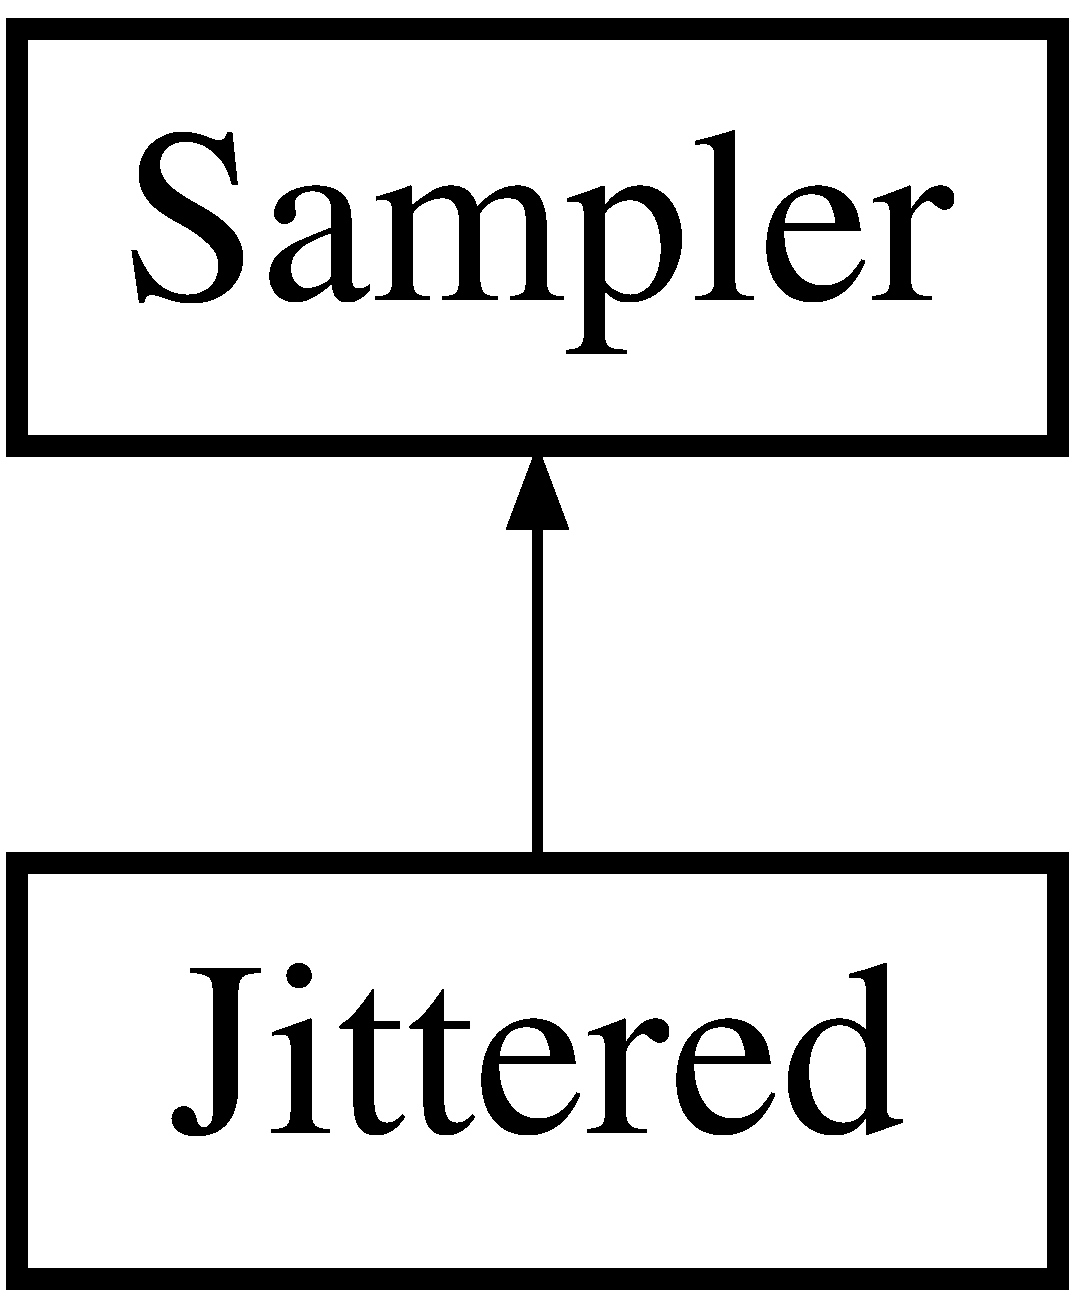
\includegraphics[height=2.000000cm]{class_jittered}
\end{center}
\end{figure}
\subsection*{Public Member Functions}
\begin{DoxyCompactItemize}
\item 
\hyperlink{class_jittered_af6b4c1f329b76db2e866145b7b506bc0}{Jittered} ()
\item 
\hyperlink{class_jittered_a140ae4562e7db9133bb1953e2f8e5ea8}{Jittered} (const int num\+Samples)
\item 
\hyperlink{class_jittered_a37413740ae17ca91a2dd02375a5683ce}{Jittered} (const int num\+Samples, const int num\+Sets)
\end{DoxyCompactItemize}
\subsection*{Additional Inherited Members}


\subsection{Detailed Description}
T\+O\+DO \begin{DoxyRemark}{Remarks}
T\+O\+DO. 
\end{DoxyRemark}


\subsection{Constructor \& Destructor Documentation}
\hypertarget{class_jittered_af6b4c1f329b76db2e866145b7b506bc0}{}\label{class_jittered_af6b4c1f329b76db2e866145b7b506bc0} 
\index{Jittered@{Jittered}!Jittered@{Jittered}}
\index{Jittered@{Jittered}!Jittered@{Jittered}}
\subsubsection{\texorpdfstring{Jittered()}{Jittered()}\hspace{0.1cm}{\footnotesize\ttfamily [1/3]}}
{\footnotesize\ttfamily Jittered\+::\+Jittered (\begin{DoxyParamCaption}{ }\end{DoxyParamCaption})}

Standard constructor. \hypertarget{class_jittered_a140ae4562e7db9133bb1953e2f8e5ea8}{}\label{class_jittered_a140ae4562e7db9133bb1953e2f8e5ea8} 
\index{Jittered@{Jittered}!Jittered@{Jittered}}
\index{Jittered@{Jittered}!Jittered@{Jittered}}
\subsubsection{\texorpdfstring{Jittered()}{Jittered()}\hspace{0.1cm}{\footnotesize\ttfamily [2/3]}}
{\footnotesize\ttfamily Jittered\+::\+Jittered (\begin{DoxyParamCaption}\item[{const int}]{num\+Samples }\end{DoxyParamCaption})}

Constructs a sampler and sets its number of samples. 
\begin{DoxyParams}{Parameters}
{\em num\+Samples} & Number of samples. \\
\hline
\end{DoxyParams}
\hypertarget{class_jittered_a37413740ae17ca91a2dd02375a5683ce}{}\label{class_jittered_a37413740ae17ca91a2dd02375a5683ce} 
\index{Jittered@{Jittered}!Jittered@{Jittered}}
\index{Jittered@{Jittered}!Jittered@{Jittered}}
\subsubsection{\texorpdfstring{Jittered()}{Jittered()}\hspace{0.1cm}{\footnotesize\ttfamily [3/3]}}
{\footnotesize\ttfamily Jittered\+::\+Jittered (\begin{DoxyParamCaption}\item[{const int}]{num\+Samples,  }\item[{const int}]{num\+Sets }\end{DoxyParamCaption})}

Constructs a sampler and sets its number of samples and sets. 
\begin{DoxyParams}{Parameters}
{\em num\+Samples} & Number of samples. \\
\hline
{\em num\+Sets} & Number of sets. \\
\hline
\end{DoxyParams}


The documentation for this class was generated from the following file\+:\begin{DoxyCompactItemize}
\item 
Source/\+Samplers/include/\hyperlink{_jittered_8h}{Jittered.\+h}\end{DoxyCompactItemize}

\hypertarget{class_lambertian}{}\section{Lambertian Class Reference}
\label{class_lambertian}\index{Lambertian@{Lambertian}}


{\ttfamily \#include $<$Lambertian.\+h$>$}

Inheritance diagram for Lambertian\+:\begin{figure}[H]
\begin{center}
\leavevmode
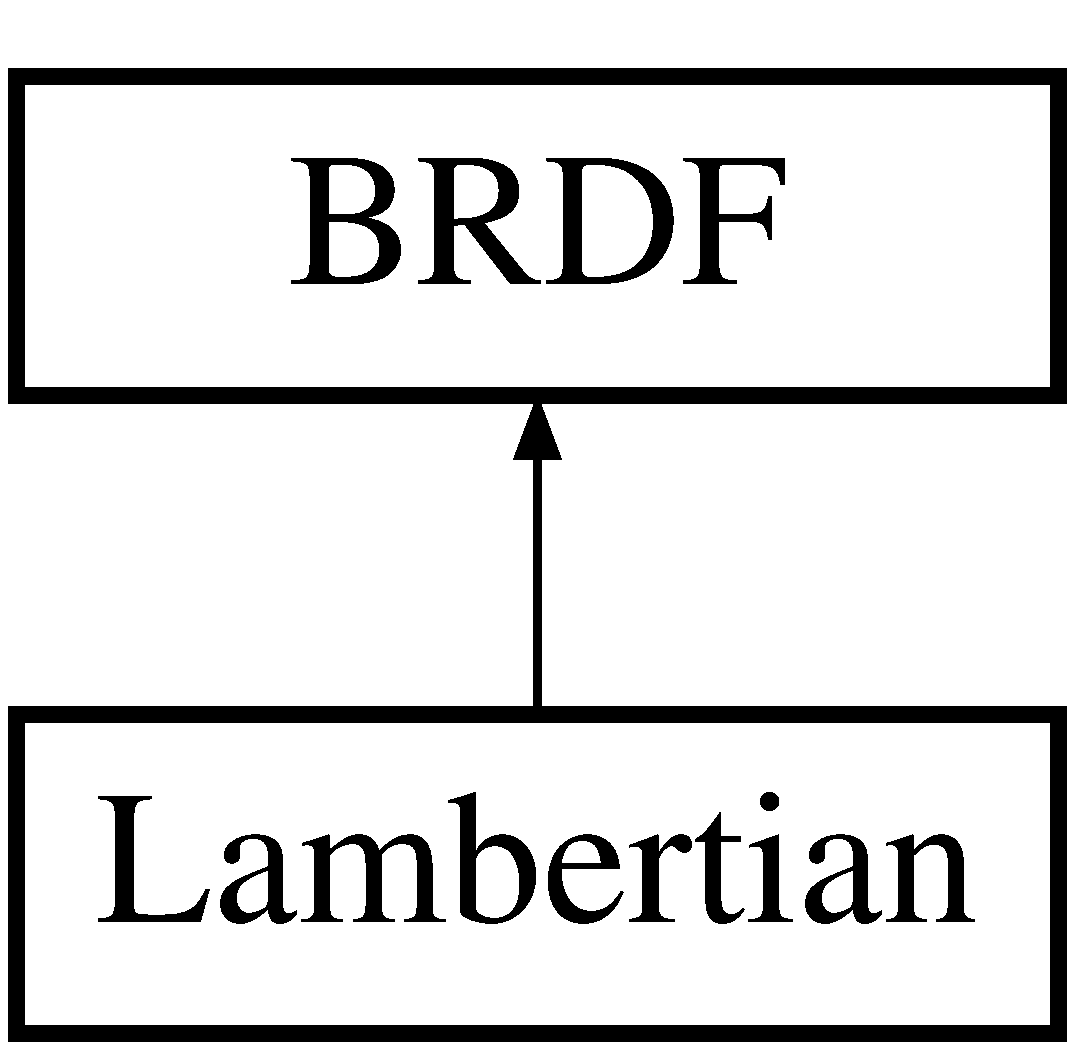
\includegraphics[height=2.000000cm]{class_lambertian}
\end{center}
\end{figure}
\subsection*{Public Member Functions}
\begin{DoxyCompactItemize}
\item 
\hyperlink{class_lambertian_a9a6eb485fd890f0873ed144ed8cbbfb2}{Lambertian} ()
\item 
virtual \hyperlink{class_r_g_b_color}{R\+G\+B\+Color} \hyperlink{group___b_r_d_f_gad7b8c290aaacbe6c11ee62529dd7389b}{f} (const \hyperlink{class_surface}{Surface} \&sr, const glm\+::vec3 \&wi, const glm\+::vec3 \&wo) const
\item 
virtual \hyperlink{class_r_g_b_color}{R\+G\+B\+Color} \hyperlink{group___b_r_d_f_gaa70272886cbeb0f91c629ace938dd0a0}{rho} (const \hyperlink{class_surface}{Surface} \&sr, const glm\+::vec3 \&wo) const
\item 
void \hyperlink{group___b_r_d_f_ga4d1bf71e27d8eacc273d244e01fe2d46}{Set\+Diffuse\+Reflection} (const float kdr)
\item 
void \hyperlink{group___b_r_d_f_gadd1e0590ffcada37b485b985182439de}{Set\+Diffuse\+Color} (const \hyperlink{class_r_g_b_color}{R\+G\+B\+Color} \&color)
\end{DoxyCompactItemize}
\subsection*{Additional Inherited Members}


\subsection{Detailed Description}
The perfect diffuse bidirectional reflectance distribution function abstraction. \begin{DoxyRemark}{Remarks}
T\+O\+DO. 
\end{DoxyRemark}


\subsection{Constructor \& Destructor Documentation}
\hypertarget{class_lambertian_a9a6eb485fd890f0873ed144ed8cbbfb2}{}\label{class_lambertian_a9a6eb485fd890f0873ed144ed8cbbfb2} 
\index{Lambertian@{Lambertian}!Lambertian@{Lambertian}}
\index{Lambertian@{Lambertian}!Lambertian@{Lambertian}}
\subsubsection{\texorpdfstring{Lambertian()}{Lambertian()}}
{\footnotesize\ttfamily Lambertian\+::\+Lambertian (\begin{DoxyParamCaption}{ }\end{DoxyParamCaption})}

Standard constructor. 

The documentation for this class was generated from the following file\+:\begin{DoxyCompactItemize}
\item 
Source/\+B\+R\+D\+Fs/include/\hyperlink{_lambertian_8h}{Lambertian.\+h}\end{DoxyCompactItemize}

\hypertarget{class_light}{}\section{Light Class Reference}
\label{class_light}\index{Light@{Light}}


{\ttfamily \#include $<$Light.\+h$>$}

Inheritance diagram for Light\+:\begin{figure}[H]
\begin{center}
\leavevmode
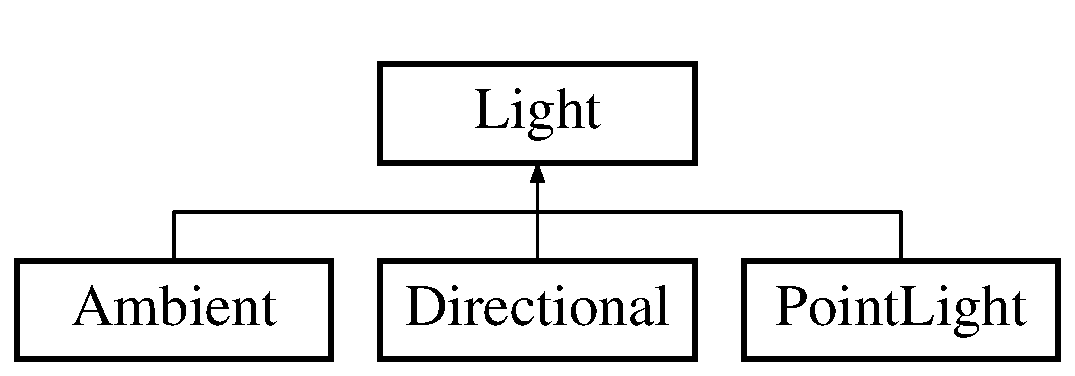
\includegraphics[height=2.000000cm]{class_light}
\end{center}
\end{figure}
\subsection*{Public Member Functions}
\begin{DoxyCompactItemize}
\item 
\hyperlink{class_light_aeb5df09a25a32f19fdffa761268ba24f}{Light} ()
\item 
virtual glm\+::vec3 \hyperlink{class_light_a62c5f73131ca1cdd6b2477f36c242482}{Get\+Direction} (\hyperlink{class_surface}{Surface} \&sr)=0
\item 
virtual \hyperlink{class_r_g_b_color}{R\+G\+B\+Color} \hyperlink{class_light_aba4ca1dcd52876cb5bee71ac8f684af5}{L} (\hyperlink{class_surface}{Surface} \&sr)
\item 
virtual bool \hyperlink{class_light_ac96c5efcdccb339609c7d19ea6ac5d17}{Shadowed} (const \hyperlink{class_ray}{Ray} \&ray, const \hyperlink{class_surface}{Surface} \&sr) const =0
\item 
void \hyperlink{group___lights_ga87d9f95e8a6d77b8fd8383b68daa23ff}{Casts\+Shadows} (bool flag)
\item 
bool \hyperlink{group___lights_gad1397ab09ba91ed92dbbeb0c8fa8bedc}{Casts\+Shadows} () const
\end{DoxyCompactItemize}
\subsection*{Protected Attributes}
\begin{DoxyCompactItemize}
\item 
bool \hyperlink{class_light_a84dea3da6749bb4ee4b141744344b403}{m\+\_\+\+Shadows}
\end{DoxyCompactItemize}


\subsection{Detailed Description}
Representation of a light source. \begin{DoxyRemark}{Remarks}
T\+O\+DO 
\end{DoxyRemark}


\subsection{Constructor \& Destructor Documentation}
\hypertarget{class_light_aeb5df09a25a32f19fdffa761268ba24f}{}\label{class_light_aeb5df09a25a32f19fdffa761268ba24f} 
\index{Light@{Light}!Light@{Light}}
\index{Light@{Light}!Light@{Light}}
\subsubsection{\texorpdfstring{Light()}{Light()}}
{\footnotesize\ttfamily Light\+::\+Light (\begin{DoxyParamCaption}{ }\end{DoxyParamCaption})}

Standard constructor. 

\subsection{Member Function Documentation}
\hypertarget{class_light_a62c5f73131ca1cdd6b2477f36c242482}{}\label{class_light_a62c5f73131ca1cdd6b2477f36c242482} 
\index{Light@{Light}!Get\+Direction@{Get\+Direction}}
\index{Get\+Direction@{Get\+Direction}!Light@{Light}}
\subsubsection{\texorpdfstring{Get\+Direction()}{GetDirection()}}
{\footnotesize\ttfamily virtual glm\+::vec3 Light\+::\+Get\+Direction (\begin{DoxyParamCaption}\item[{\hyperlink{class_surface}{Surface} \&}]{sr }\end{DoxyParamCaption})\hspace{0.3cm}{\ttfamily [pure virtual]}}

Computes the direction of the incoming light at a given surface. 
\begin{DoxyParams}{Parameters}
{\em sr} & Information about the surface of the object. \\
\hline
\end{DoxyParams}
\begin{DoxyReturn}{Returns}
Direction from which the light arrives at the surface. 
\end{DoxyReturn}


Implemented in \hyperlink{class_ambient_acb2fc1574883ea0bd41c662ec904164f}{Ambient}, \hyperlink{class_directional_a022fc1cb35f0f760b5472c06ad6e2e74}{Directional}, and \hyperlink{class_point_light_af587fd5a2e72f32fcf5041a2cfb055e1}{Point\+Light}.

\hypertarget{class_light_aba4ca1dcd52876cb5bee71ac8f684af5}{}\label{class_light_aba4ca1dcd52876cb5bee71ac8f684af5} 
\index{Light@{Light}!L@{L}}
\index{L@{L}!Light@{Light}}
\subsubsection{\texorpdfstring{L()}{L()}}
{\footnotesize\ttfamily virtual \hyperlink{class_r_g_b_color}{R\+G\+B\+Color} Light\+::L (\begin{DoxyParamCaption}\item[{\hyperlink{class_surface}{Surface} \&}]{sr }\end{DoxyParamCaption})\hspace{0.3cm}{\ttfamily [virtual]}}

Computes the incident radiance at a given surface. 
\begin{DoxyParams}{Parameters}
{\em sr} & Information about the surface of the object. \\
\hline
\end{DoxyParams}
\begin{DoxyReturn}{Returns}
Incident radiance at the surface. 
\end{DoxyReturn}


Reimplemented in \hyperlink{class_ambient_aa75478ba2b30c9930ef538dd16f4586a}{Ambient}, \hyperlink{class_directional_ac9a728a89d32c5f62ddef2be6c3e467d}{Directional}, and \hyperlink{class_point_light_a0d5e1227bc28f5a26edb595fe443f7f3}{Point\+Light}.

\hypertarget{class_light_ac96c5efcdccb339609c7d19ea6ac5d17}{}\label{class_light_ac96c5efcdccb339609c7d19ea6ac5d17} 
\index{Light@{Light}!Shadowed@{Shadowed}}
\index{Shadowed@{Shadowed}!Light@{Light}}
\subsubsection{\texorpdfstring{Shadowed()}{Shadowed()}}
{\footnotesize\ttfamily virtual bool Light\+::\+Shadowed (\begin{DoxyParamCaption}\item[{const \hyperlink{class_ray}{Ray} \&}]{ray,  }\item[{const \hyperlink{class_surface}{Surface} \&}]{sr }\end{DoxyParamCaption}) const\hspace{0.3cm}{\ttfamily [pure virtual]}}

Checks if a surface is shadowed by another object. 
\begin{DoxyParams}{Parameters}
{\em ray} & Casted shadow ray. \\
\hline
{\em sr} & Information about the surface of the object. \\
\hline
\end{DoxyParams}
\begin{DoxyReturn}{Returns}
True, if the surface is shadowed. 
\end{DoxyReturn}


Implemented in \hyperlink{class_ambient_a1373251f8db560b10061eb23f125bb27}{Ambient}, \hyperlink{class_directional_a56a42abcdb41df1e3dd44b173aee494a}{Directional}, and \hyperlink{class_point_light_aa4a50b149cdc22acbf2140a7e2ff9551}{Point\+Light}.



\subsection{Member Data Documentation}
\hypertarget{class_light_a84dea3da6749bb4ee4b141744344b403}{}\label{class_light_a84dea3da6749bb4ee4b141744344b403} 
\index{Light@{Light}!m\+\_\+\+Shadows@{m\+\_\+\+Shadows}}
\index{m\+\_\+\+Shadows@{m\+\_\+\+Shadows}!Light@{Light}}
\subsubsection{\texorpdfstring{m\+\_\+\+Shadows}{m\_Shadows}}
{\footnotesize\ttfamily bool Light\+::m\+\_\+\+Shadows\hspace{0.3cm}{\ttfamily [protected]}}

Flag that stores information about whether the objects illuminated by the light casts shadows over other objects. 

The documentation for this class was generated from the following file\+:\begin{DoxyCompactItemize}
\item 
Source/\+Lights/include/\hyperlink{_light_8h}{Light.\+h}\end{DoxyCompactItemize}

\hypertarget{class_material}{}\section{Material Class Reference}
\label{class_material}\index{Material@{Material}}


{\ttfamily \#include $<$Material.\+h$>$}

Inheritance diagram for Material\+:\begin{figure}[H]
\begin{center}
\leavevmode
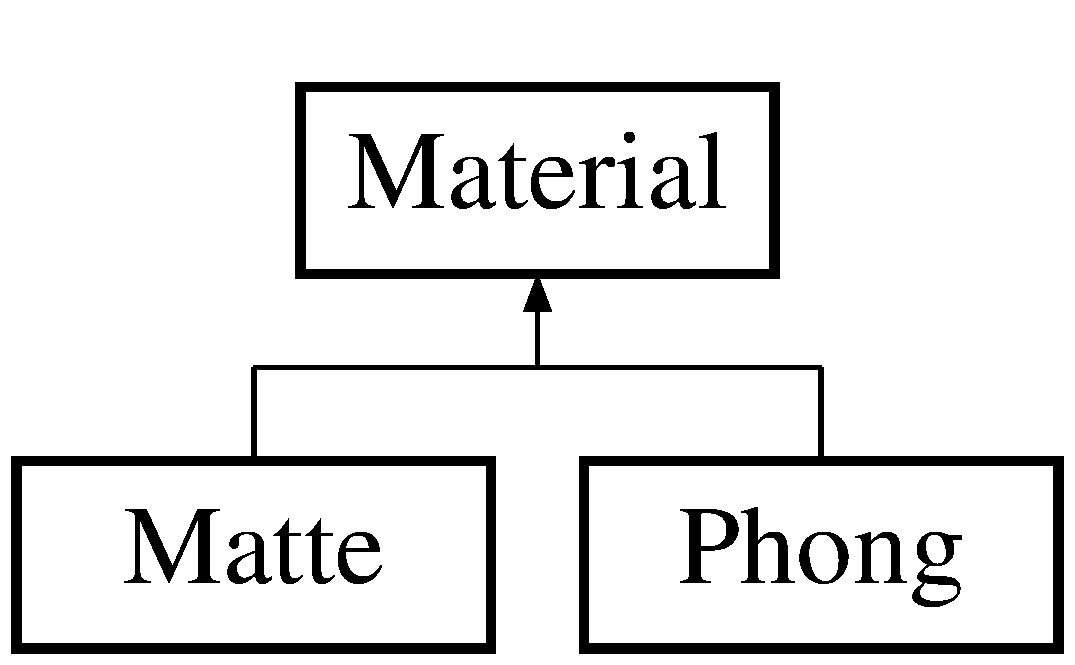
\includegraphics[height=2.000000cm]{class_material}
\end{center}
\end{figure}
\subsection*{Public Member Functions}
\begin{DoxyCompactItemize}
\item 
\hyperlink{class_material_a137e987401b63eb7c6c27c3e38bc74b5}{Material} ()
\item 
virtual \hyperlink{class_r_g_b_color}{R\+G\+B\+Color} \hyperlink{class_material_aeccd880ee7b86a849e8f2d2f0bcf4fc7}{Shade} (\hyperlink{class_surface}{Surface} \&sr) const
\end{DoxyCompactItemize}


\subsection{Detailed Description}
Rendering properties of an object. \begin{DoxyRemark}{Remarks}
T\+O\+DO. 
\end{DoxyRemark}


\subsection{Constructor \& Destructor Documentation}
\hypertarget{class_material_a137e987401b63eb7c6c27c3e38bc74b5}{}\label{class_material_a137e987401b63eb7c6c27c3e38bc74b5} 
\index{Material@{Material}!Material@{Material}}
\index{Material@{Material}!Material@{Material}}
\subsubsection{\texorpdfstring{Material()}{Material()}}
{\footnotesize\ttfamily Material\+::\+Material (\begin{DoxyParamCaption}{ }\end{DoxyParamCaption})}

Standard constructor. 

\subsection{Member Function Documentation}
\hypertarget{class_material_aeccd880ee7b86a849e8f2d2f0bcf4fc7}{}\label{class_material_aeccd880ee7b86a849e8f2d2f0bcf4fc7} 
\index{Material@{Material}!Shade@{Shade}}
\index{Shade@{Shade}!Material@{Material}}
\subsubsection{\texorpdfstring{Shade()}{Shade()}}
{\footnotesize\ttfamily virtual \hyperlink{class_r_g_b_color}{R\+G\+B\+Color} Material\+::\+Shade (\begin{DoxyParamCaption}\item[{\hyperlink{class_surface}{Surface} \&}]{sr }\end{DoxyParamCaption}) const\hspace{0.3cm}{\ttfamily [virtual]}}

Computes the color of a given surface. 
\begin{DoxyParams}{Parameters}
{\em sr} & Information about the surface of the object. \\
\hline
\end{DoxyParams}
\begin{DoxyReturn}{Returns}
Color of the surface. 
\end{DoxyReturn}


Reimplemented in \hyperlink{class_phong_a4ab7e1d4514c37abe47e18d627856dc8}{Phong}, and \hyperlink{class_matte_a1313aabd946d45ec67a9de4fbc486f6c}{Matte}.



The documentation for this class was generated from the following file\+:\begin{DoxyCompactItemize}
\item 
Source/\+Materials/include/\hyperlink{_material_8h}{Material.\+h}\end{DoxyCompactItemize}

\hypertarget{class_matte}{}\section{Matte Class Reference}
\label{class_matte}\index{Matte@{Matte}}


{\ttfamily \#include $<$Matte.\+h$>$}

Inheritance diagram for Matte\+:\begin{figure}[H]
\begin{center}
\leavevmode
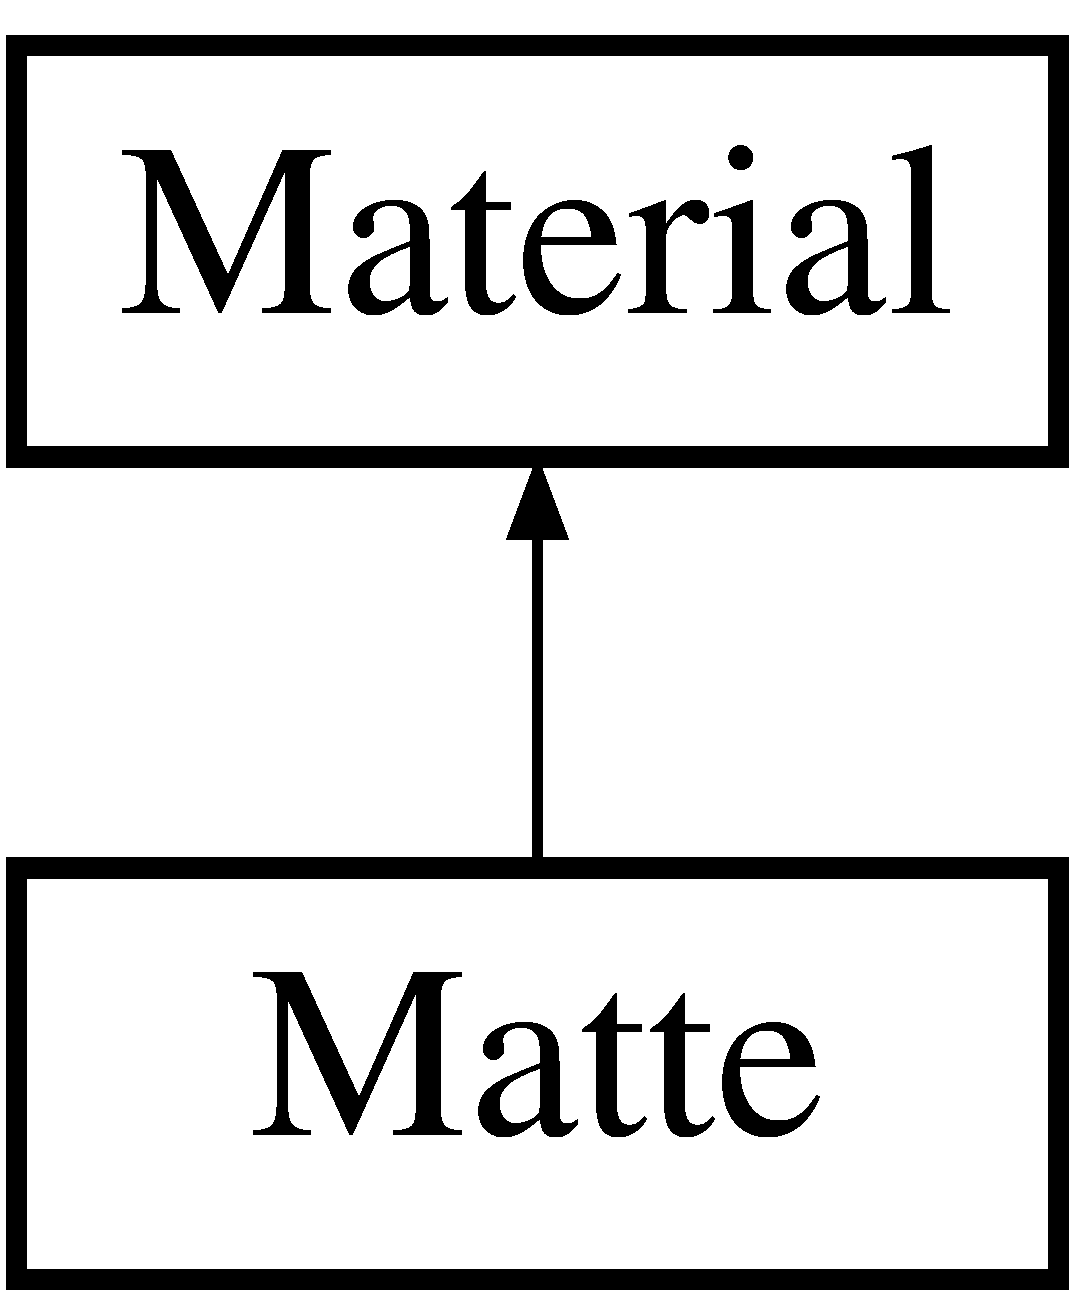
\includegraphics[height=2.000000cm]{class_matte}
\end{center}
\end{figure}
\subsection*{Public Member Functions}
\begin{DoxyCompactItemize}
\item 
\hyperlink{class_matte_a1f460cbc9dd811c509ca50b652102ac2}{Matte} ()
\item 
virtual \hyperlink{class_r_g_b_color}{R\+G\+B\+Color} \hyperlink{class_matte_a1313aabd946d45ec67a9de4fbc486f6c}{Shade} (\hyperlink{class_surface}{Surface} \&sr) const
\item 
void \hyperlink{group___materials_gad4df0e4b6f2112282b492f068faf1d72}{Set\+Ambient\+Reflection} (const float kdr)
\item 
void \hyperlink{group___materials_ga3a3fb682a6cfb419d05bf5dba9088f57}{Set\+Ambient\+Color} (const \hyperlink{class_r_g_b_color}{R\+G\+B\+Color} \&color)
\item 
void \hyperlink{group___materials_ga59c2ccdf9e80053784f5449603c7b7a3}{Set\+Diffuse\+Reflection} (const float kdr)
\item 
void \hyperlink{group___materials_ga6a82d5d8fd47aeb188380c067477e396}{Set\+Diffuse\+Color} (const \hyperlink{class_r_g_b_color}{R\+G\+B\+Color} \&color)
\item 
void \hyperlink{group___materials_ga6b42d7c8b02c61801702dc19d8e3ba5a}{Set\+Sampler} (std\+::shared\+\_\+ptr$<$ \hyperlink{class_sampler}{Sampler} $>$ sampler\+\_\+ptr)
\end{DoxyCompactItemize}


\subsection{Detailed Description}
Rendering properties of an object. \begin{DoxyRemark}{Remarks}
T\+O\+DO. 
\end{DoxyRemark}
\begin{DoxySeeAlso}{See also}
\hyperlink{class_lambertian}{Lambertian} 
\end{DoxySeeAlso}


\subsection{Constructor \& Destructor Documentation}
\hypertarget{class_matte_a1f460cbc9dd811c509ca50b652102ac2}{}\label{class_matte_a1f460cbc9dd811c509ca50b652102ac2} 
\index{Matte@{Matte}!Matte@{Matte}}
\index{Matte@{Matte}!Matte@{Matte}}
\subsubsection{\texorpdfstring{Matte()}{Matte()}}
{\footnotesize\ttfamily Matte\+::\+Matte (\begin{DoxyParamCaption}{ }\end{DoxyParamCaption})}

Standard constructor. 

\subsection{Member Function Documentation}
\hypertarget{class_matte_a1313aabd946d45ec67a9de4fbc486f6c}{}\label{class_matte_a1313aabd946d45ec67a9de4fbc486f6c} 
\index{Matte@{Matte}!Shade@{Shade}}
\index{Shade@{Shade}!Matte@{Matte}}
\subsubsection{\texorpdfstring{Shade()}{Shade()}}
{\footnotesize\ttfamily virtual \hyperlink{class_r_g_b_color}{R\+G\+B\+Color} Matte\+::\+Shade (\begin{DoxyParamCaption}\item[{\hyperlink{class_surface}{Surface} \&}]{sr }\end{DoxyParamCaption}) const\hspace{0.3cm}{\ttfamily [virtual]}}

Computes the color of a given surface. 
\begin{DoxyParams}{Parameters}
{\em sr} & Information about the surface of the object. \\
\hline
\end{DoxyParams}
\begin{DoxyReturn}{Returns}
Color of the surface. 
\end{DoxyReturn}


Reimplemented from \hyperlink{class_material_aeccd880ee7b86a849e8f2d2f0bcf4fc7}{Material}.



The documentation for this class was generated from the following file\+:\begin{DoxyCompactItemize}
\item 
Source/\+Materials/include/\hyperlink{_matte_8h}{Matte.\+h}\end{DoxyCompactItemize}

\hypertarget{class_multi_jittered}{}\section{Multi\+Jittered Class Reference}
\label{class_multi_jittered}\index{Multi\+Jittered@{Multi\+Jittered}}


{\ttfamily \#include $<$Multi\+Jittered.\+h$>$}

Inheritance diagram for Multi\+Jittered\+:\begin{figure}[H]
\begin{center}
\leavevmode
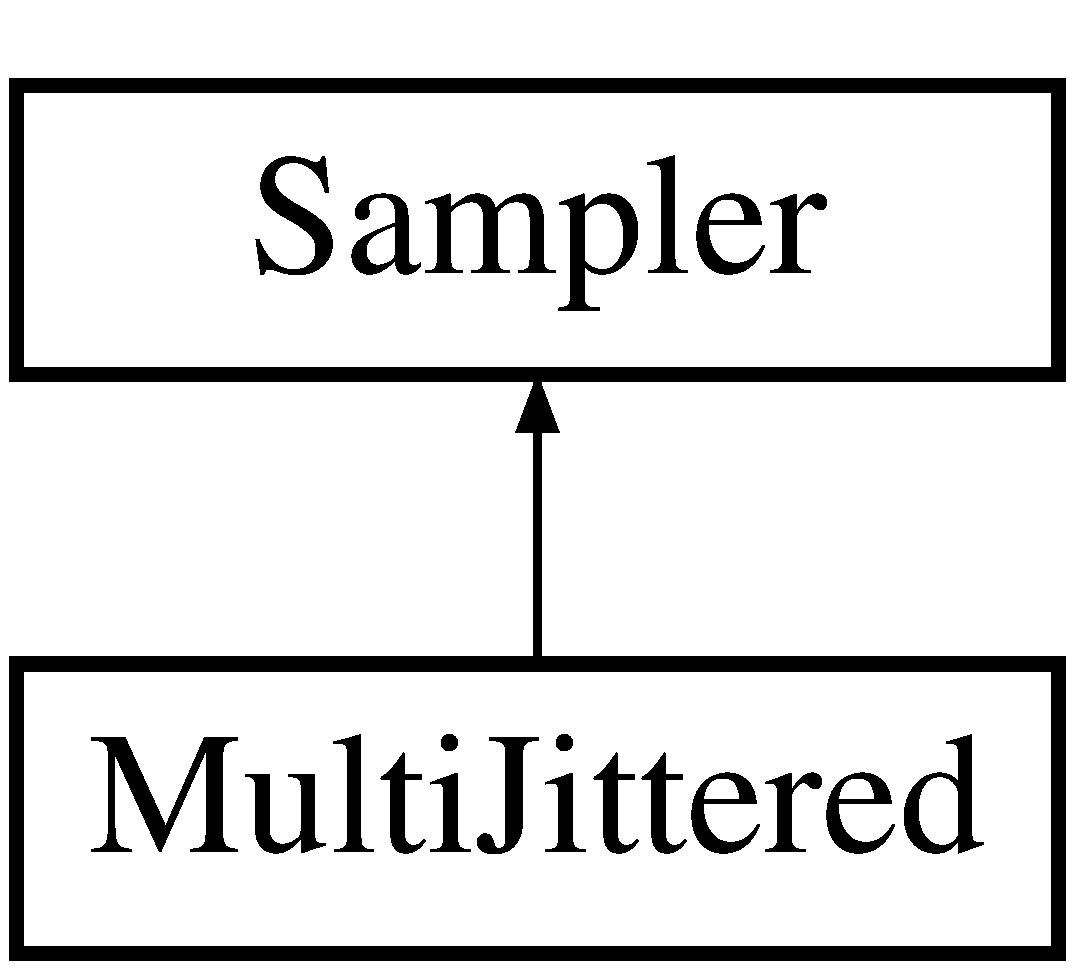
\includegraphics[height=2.000000cm]{class_multi_jittered}
\end{center}
\end{figure}
\subsection*{Public Member Functions}
\begin{DoxyCompactItemize}
\item 
\hyperlink{class_multi_jittered_a2480bb454a04e682683cb302567cbd55}{Multi\+Jittered} ()
\item 
\hyperlink{class_multi_jittered_a6788f23e84fc6ae4029c7fd408c8e671}{Multi\+Jittered} (const int num\+Samples)
\item 
\hyperlink{class_multi_jittered_a8b59445dea3b73a787082f8d2f5fb8b9}{Multi\+Jittered} (const int num\+Samples, const int num\+Sets)
\end{DoxyCompactItemize}
\subsection*{Additional Inherited Members}


\subsection{Detailed Description}
T\+O\+DO \begin{DoxyRemark}{Remarks}
T\+O\+DO. 
\end{DoxyRemark}


\subsection{Constructor \& Destructor Documentation}
\hypertarget{class_multi_jittered_a2480bb454a04e682683cb302567cbd55}{}\label{class_multi_jittered_a2480bb454a04e682683cb302567cbd55} 
\index{Multi\+Jittered@{Multi\+Jittered}!Multi\+Jittered@{Multi\+Jittered}}
\index{Multi\+Jittered@{Multi\+Jittered}!Multi\+Jittered@{Multi\+Jittered}}
\subsubsection{\texorpdfstring{Multi\+Jittered()}{MultiJittered()}\hspace{0.1cm}{\footnotesize\ttfamily [1/3]}}
{\footnotesize\ttfamily Multi\+Jittered\+::\+Multi\+Jittered (\begin{DoxyParamCaption}{ }\end{DoxyParamCaption})}

Standard constructor. \hypertarget{class_multi_jittered_a6788f23e84fc6ae4029c7fd408c8e671}{}\label{class_multi_jittered_a6788f23e84fc6ae4029c7fd408c8e671} 
\index{Multi\+Jittered@{Multi\+Jittered}!Multi\+Jittered@{Multi\+Jittered}}
\index{Multi\+Jittered@{Multi\+Jittered}!Multi\+Jittered@{Multi\+Jittered}}
\subsubsection{\texorpdfstring{Multi\+Jittered()}{MultiJittered()}\hspace{0.1cm}{\footnotesize\ttfamily [2/3]}}
{\footnotesize\ttfamily Multi\+Jittered\+::\+Multi\+Jittered (\begin{DoxyParamCaption}\item[{const int}]{num\+Samples }\end{DoxyParamCaption})}

Constructs a sampler and sets its number of samples. 
\begin{DoxyParams}{Parameters}
{\em num\+Samples} & Number of samples. \\
\hline
\end{DoxyParams}
\hypertarget{class_multi_jittered_a8b59445dea3b73a787082f8d2f5fb8b9}{}\label{class_multi_jittered_a8b59445dea3b73a787082f8d2f5fb8b9} 
\index{Multi\+Jittered@{Multi\+Jittered}!Multi\+Jittered@{Multi\+Jittered}}
\index{Multi\+Jittered@{Multi\+Jittered}!Multi\+Jittered@{Multi\+Jittered}}
\subsubsection{\texorpdfstring{Multi\+Jittered()}{MultiJittered()}\hspace{0.1cm}{\footnotesize\ttfamily [3/3]}}
{\footnotesize\ttfamily Multi\+Jittered\+::\+Multi\+Jittered (\begin{DoxyParamCaption}\item[{const int}]{num\+Samples,  }\item[{const int}]{num\+Sets }\end{DoxyParamCaption})}

Constructs a sampler and sets its number of samples and sets. 
\begin{DoxyParams}{Parameters}
{\em num\+Samples} & Number of samples. \\
\hline
{\em num\+Sets} & Number of sets. \\
\hline
\end{DoxyParams}


The documentation for this class was generated from the following file\+:\begin{DoxyCompactItemize}
\item 
Source/\+Samplers/include/\hyperlink{_multi_jittered_8h}{Multi\+Jittered.\+h}\end{DoxyCompactItemize}

\hypertarget{class_multiple_objects}{}\section{Multiple\+Objects Class Reference}
\label{class_multiple_objects}\index{Multiple\+Objects@{Multiple\+Objects}}


{\ttfamily \#include $<$Multiple\+Objects.\+h$>$}

Inheritance diagram for Multiple\+Objects\+:\begin{figure}[H]
\begin{center}
\leavevmode
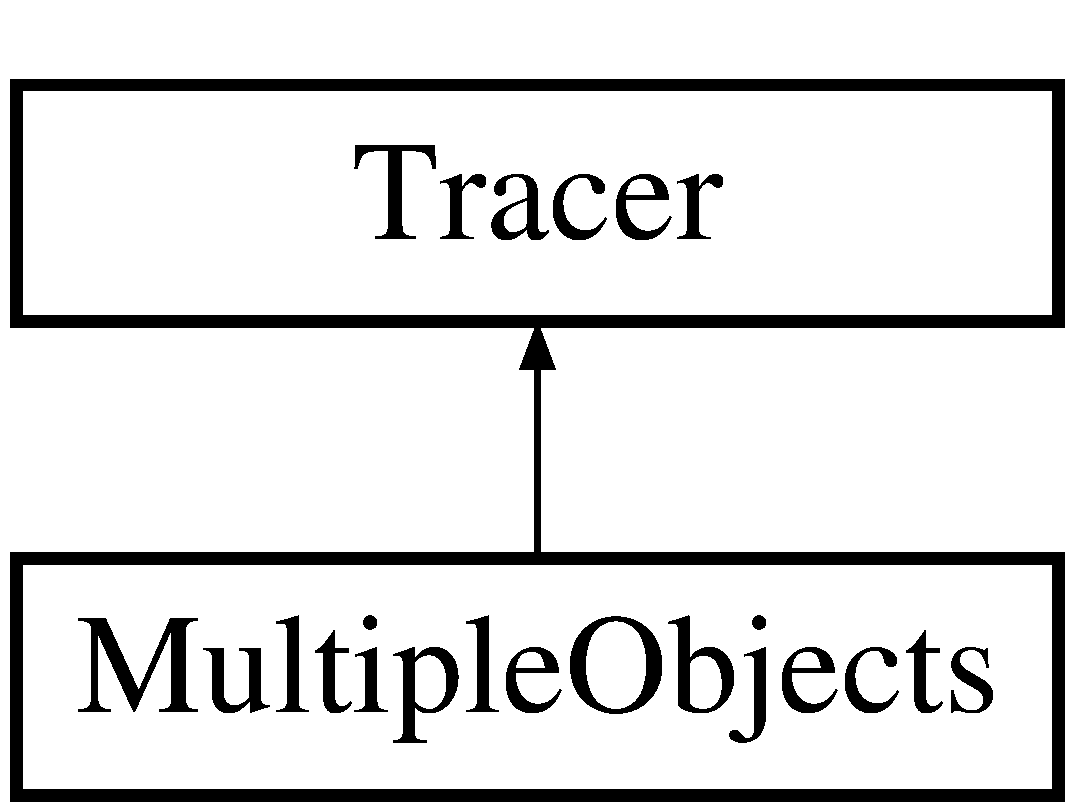
\includegraphics[height=2.000000cm]{class_multiple_objects}
\end{center}
\end{figure}
\subsection*{Public Member Functions}
\begin{DoxyCompactItemize}
\item 
\hyperlink{class_multiple_objects_a1d94b26c47ff2ab79c3471e0f8129ead}{Multiple\+Objects} (std\+::shared\+\_\+ptr$<$ World $>$)
\item 
virtual \hyperlink{class_r_g_b_color}{R\+G\+B\+Color} \hyperlink{class_multiple_objects_a46206cc6dd09a9c587e33ac896bc8e3a}{Trace\+Ray} (const \hyperlink{class_ray}{Ray} \&) const
\end{DoxyCompactItemize}
\subsection*{Additional Inherited Members}


\subsection{Constructor \& Destructor Documentation}
\hypertarget{class_multiple_objects_a1d94b26c47ff2ab79c3471e0f8129ead}{}\label{class_multiple_objects_a1d94b26c47ff2ab79c3471e0f8129ead} 
\index{Multiple\+Objects@{Multiple\+Objects}!Multiple\+Objects@{Multiple\+Objects}}
\index{Multiple\+Objects@{Multiple\+Objects}!Multiple\+Objects@{Multiple\+Objects}}
\subsubsection{\texorpdfstring{Multiple\+Objects()}{MultipleObjects()}}
{\footnotesize\ttfamily Multiple\+Objects\+::\+Multiple\+Objects (\begin{DoxyParamCaption}\item[{std\+::shared\+\_\+ptr$<$ World $>$}]{ }\end{DoxyParamCaption})}

Constructs a \hyperlink{class_tracer}{Tracer} with a pointer to the world. 
\begin{DoxyParams}{Parameters}
{\em \{std\+::shared\+\_\+ptr$<$\+World$>$\}} & world\+\_\+ptr Pointer to the world. \\
\hline
\end{DoxyParams}


\subsection{Member Function Documentation}
\hypertarget{class_multiple_objects_a46206cc6dd09a9c587e33ac896bc8e3a}{}\label{class_multiple_objects_a46206cc6dd09a9c587e33ac896bc8e3a} 
\index{Multiple\+Objects@{Multiple\+Objects}!Trace\+Ray@{Trace\+Ray}}
\index{Trace\+Ray@{Trace\+Ray}!Multiple\+Objects@{Multiple\+Objects}}
\subsubsection{\texorpdfstring{Trace\+Ray()}{TraceRay()}}
{\footnotesize\ttfamily virtual \hyperlink{class_r_g_b_color}{R\+G\+B\+Color} Multiple\+Objects\+::\+Trace\+Ray (\begin{DoxyParamCaption}\item[{const \hyperlink{class_ray}{Ray} \&}]{ }\end{DoxyParamCaption}) const\hspace{0.3cm}{\ttfamily [virtual]}}

Standard ray tracing method. 
\begin{DoxyParams}{Parameters}
{\em \{const} & \hyperlink{class_ray}{Ray} \&\} ray \hyperlink{class_ray}{Ray} traced. \\
\hline
\end{DoxyParams}
\begin{DoxyReturn}{Returns}
\{\hyperlink{class_r_g_b_color}{R\+G\+B\+Color}\} 
\end{DoxyReturn}


Reimplemented from \hyperlink{class_tracer_adbabdfde11e278945a0433d08445fcce}{Tracer}.



The documentation for this class was generated from the following file\+:\begin{DoxyCompactItemize}
\item 
Source/\+Tracers/include/\hyperlink{_multiple_objects_8h}{Multiple\+Objects.\+h}\end{DoxyCompactItemize}

\hypertarget{class_n_rooks}{}\section{N\+Rooks Class Reference}
\label{class_n_rooks}\index{N\+Rooks@{N\+Rooks}}


{\ttfamily \#include $<$N\+Rooks.\+h$>$}

Inheritance diagram for N\+Rooks\+:\begin{figure}[H]
\begin{center}
\leavevmode
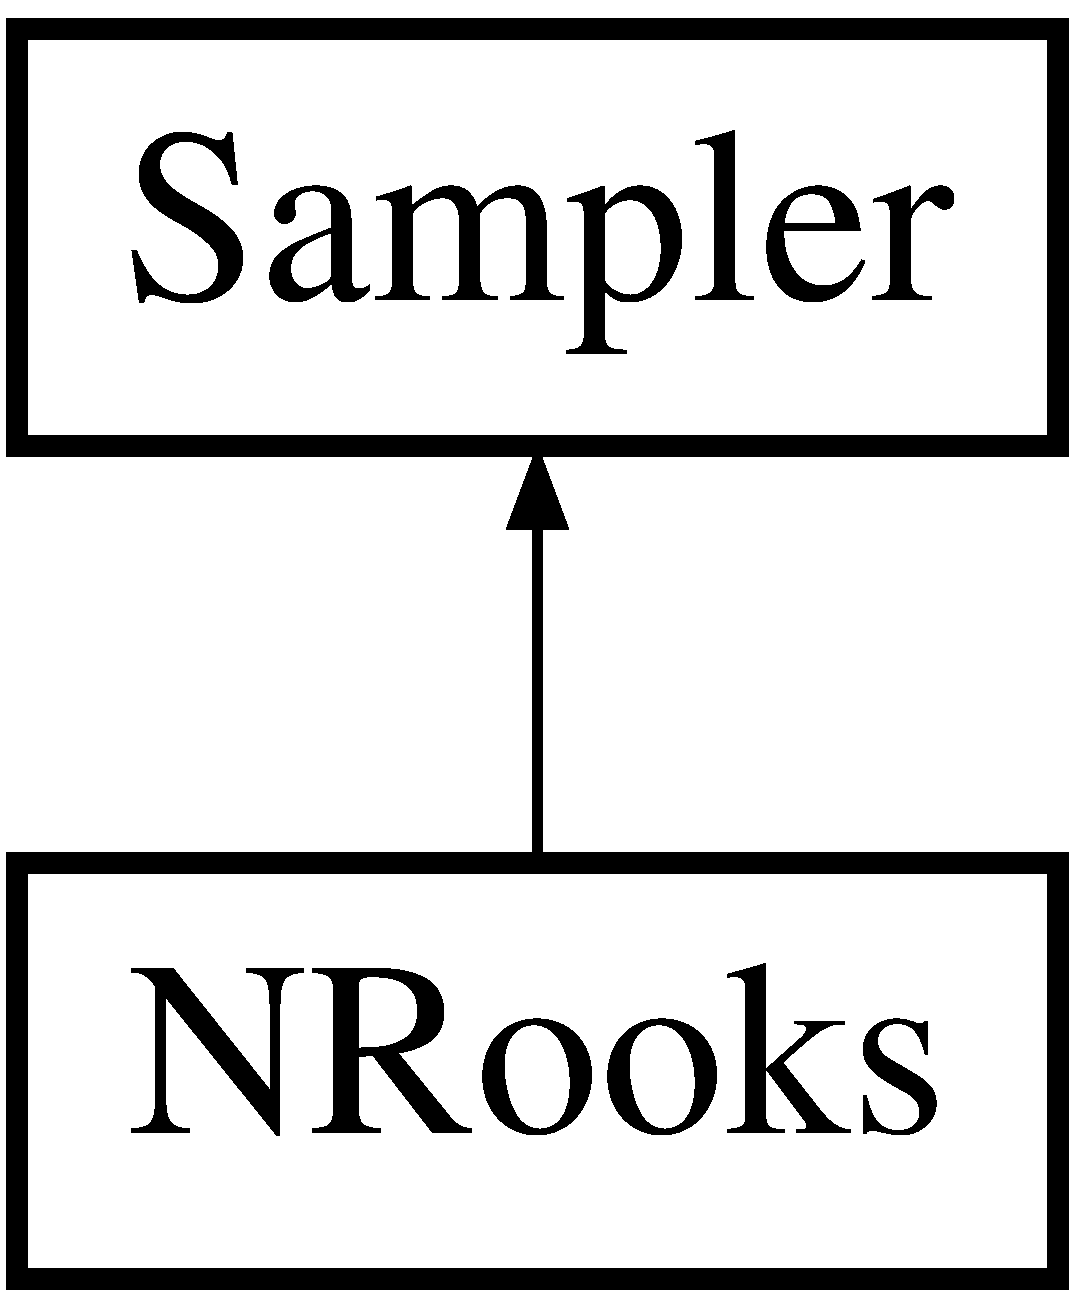
\includegraphics[height=2.000000cm]{class_n_rooks}
\end{center}
\end{figure}
\subsection*{Public Member Functions}
\begin{DoxyCompactItemize}
\item 
\hyperlink{class_n_rooks_af718469f67388fb083d7c140347dd90e}{N\+Rooks} ()
\item 
\hyperlink{class_n_rooks_a927f85bd26be336f880f9b4e033d1cea}{N\+Rooks} (const int num\+Samples)
\item 
\hyperlink{class_n_rooks_a79ca631d81a4b42d319cd2582bb39d8c}{N\+Rooks} (const int num\+Samples, const int num\+Sets)
\end{DoxyCompactItemize}
\subsection*{Additional Inherited Members}


\subsection{Detailed Description}
T\+O\+DO \begin{DoxyRemark}{Remarks}
T\+O\+DO. 
\end{DoxyRemark}


\subsection{Constructor \& Destructor Documentation}
\hypertarget{class_n_rooks_af718469f67388fb083d7c140347dd90e}{}\label{class_n_rooks_af718469f67388fb083d7c140347dd90e} 
\index{N\+Rooks@{N\+Rooks}!N\+Rooks@{N\+Rooks}}
\index{N\+Rooks@{N\+Rooks}!N\+Rooks@{N\+Rooks}}
\subsubsection{\texorpdfstring{N\+Rooks()}{NRooks()}\hspace{0.1cm}{\footnotesize\ttfamily [1/3]}}
{\footnotesize\ttfamily N\+Rooks\+::\+N\+Rooks (\begin{DoxyParamCaption}{ }\end{DoxyParamCaption})}

Standard constructor. \hypertarget{class_n_rooks_a927f85bd26be336f880f9b4e033d1cea}{}\label{class_n_rooks_a927f85bd26be336f880f9b4e033d1cea} 
\index{N\+Rooks@{N\+Rooks}!N\+Rooks@{N\+Rooks}}
\index{N\+Rooks@{N\+Rooks}!N\+Rooks@{N\+Rooks}}
\subsubsection{\texorpdfstring{N\+Rooks()}{NRooks()}\hspace{0.1cm}{\footnotesize\ttfamily [2/3]}}
{\footnotesize\ttfamily N\+Rooks\+::\+N\+Rooks (\begin{DoxyParamCaption}\item[{const int}]{num\+Samples }\end{DoxyParamCaption})}

Constructs a sampler and sets its number of samples. 
\begin{DoxyParams}{Parameters}
{\em num\+Samples} & Number of samples. \\
\hline
\end{DoxyParams}
\hypertarget{class_n_rooks_a79ca631d81a4b42d319cd2582bb39d8c}{}\label{class_n_rooks_a79ca631d81a4b42d319cd2582bb39d8c} 
\index{N\+Rooks@{N\+Rooks}!N\+Rooks@{N\+Rooks}}
\index{N\+Rooks@{N\+Rooks}!N\+Rooks@{N\+Rooks}}
\subsubsection{\texorpdfstring{N\+Rooks()}{NRooks()}\hspace{0.1cm}{\footnotesize\ttfamily [3/3]}}
{\footnotesize\ttfamily N\+Rooks\+::\+N\+Rooks (\begin{DoxyParamCaption}\item[{const int}]{num\+Samples,  }\item[{const int}]{num\+Sets }\end{DoxyParamCaption})}

Constructs a sampler and sets its number of samples and sets. 
\begin{DoxyParams}{Parameters}
{\em num\+Samples} & Number of samples. \\
\hline
{\em num\+Sets} & Number of sets. \\
\hline
\end{DoxyParams}


The documentation for this class was generated from the following file\+:\begin{DoxyCompactItemize}
\item 
Source/\+Samplers/include/\hyperlink{_n_rooks_8h}{N\+Rooks.\+h}\end{DoxyCompactItemize}

\hypertarget{class_object}{}\section{Object Class Reference}
\label{class_object}\index{Object@{Object}}


{\ttfamily \#include $<$Object.\+h$>$}

Inheritance diagram for Object\+:\begin{figure}[H]
\begin{center}
\leavevmode
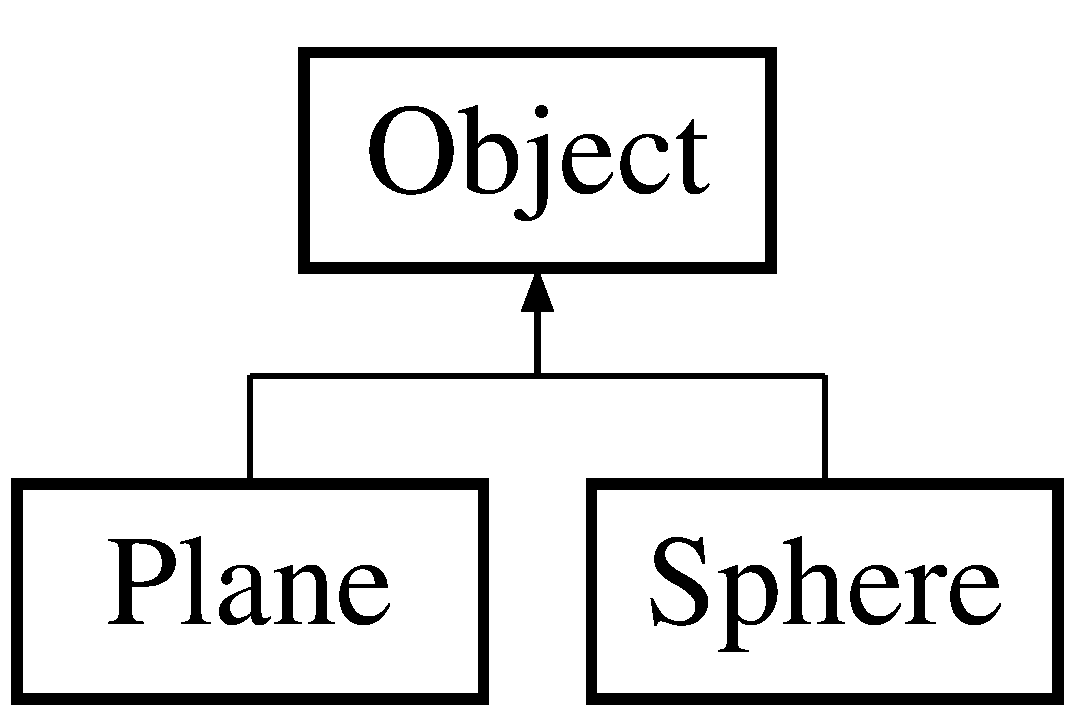
\includegraphics[height=2.000000cm]{class_object}
\end{center}
\end{figure}
\subsection*{Public Member Functions}
\begin{DoxyCompactItemize}
\item 
\hyperlink{class_object_a40860402e64d8008fb42329df7097cdb}{Object} ()
\item 
virtual bool \hyperlink{class_object_ad9977e40c0a3048eba9a81b25efcf3ef}{Hit} (const \hyperlink{class_ray}{Ray} \&ray, double \&tmin, \hyperlink{class_surface}{Surface} \&sr) const =0
\item 
virtual bool \hyperlink{class_object_a020a6edbef7b2591b1dd6815ebbc5aa0}{Shadow\+Hit} (const \hyperlink{class_ray}{Ray} \&ray, float \&tmin) const =0
\item 
void \hyperlink{group___geometric_objects_ga74fa63e74026915a261117724303adfc}{Casts\+Shadows} (bool flag)
\item 
bool \hyperlink{group___geometric_objects_gab4254fb85f166245bb7234f5c5295777}{Casts\+Shadows} () const
\item 
std\+::shared\+\_\+ptr$<$ \hyperlink{class_material}{Material} $>$ \hyperlink{group___geometric_objects_ga7ad7172879f1b2fd092561827aa2bbb1}{Get\+Material} () const
\item 
virtual void \hyperlink{class_object_a791d7431f79b030866aa31c7c29ea0db}{Set\+Material} (std\+::shared\+\_\+ptr$<$ \hyperlink{class_material}{Material} $>$ material\+\_\+ptr)
\end{DoxyCompactItemize}
\subsection*{Protected Attributes}
\begin{DoxyCompactItemize}
\item 
std\+::shared\+\_\+ptr$<$ \hyperlink{class_material}{Material} $>$ \hyperlink{class_object_aa79a61ad1ff44b1585cc4972034cecbe}{m\+\_\+\+Material\+Ptr}
\item 
bool \hyperlink{class_object_a7cde4bccf1989da90c2d2b463876e179}{m\+\_\+\+Shadows}
\end{DoxyCompactItemize}


\subsection{Detailed Description}
Holder of data of 3D objects. \begin{DoxyRemark}{Remarks}
T\+O\+DO. 
\end{DoxyRemark}


\subsection{Constructor \& Destructor Documentation}
\hypertarget{class_object_a40860402e64d8008fb42329df7097cdb}{}\label{class_object_a40860402e64d8008fb42329df7097cdb} 
\index{Object@{Object}!Object@{Object}}
\index{Object@{Object}!Object@{Object}}
\subsubsection{\texorpdfstring{Object()}{Object()}}
{\footnotesize\ttfamily Object\+::\+Object (\begin{DoxyParamCaption}{ }\end{DoxyParamCaption})}

Standard constructor. 

\subsection{Member Function Documentation}
\hypertarget{class_object_ad9977e40c0a3048eba9a81b25efcf3ef}{}\label{class_object_ad9977e40c0a3048eba9a81b25efcf3ef} 
\index{Object@{Object}!Hit@{Hit}}
\index{Hit@{Hit}!Object@{Object}}
\subsubsection{\texorpdfstring{Hit()}{Hit()}}
{\footnotesize\ttfamily virtual bool Object\+::\+Hit (\begin{DoxyParamCaption}\item[{const \hyperlink{class_ray}{Ray} \&}]{ray,  }\item[{double \&}]{tmin,  }\item[{\hyperlink{class_surface}{Surface} \&}]{sr }\end{DoxyParamCaption}) const\hspace{0.3cm}{\ttfamily [pure virtual]}}

Checks if a ray intersects with this object and return it\textquotesingle{}s shading information. 
\begin{DoxyParams}{Parameters}
{\em ray} & Intersection ray. \\
\hline
{\em tmin} & T\+O\+DO. \\
\hline
{\em sr} & Information about the surface of the object. \\
\hline
\end{DoxyParams}
\begin{DoxyReturn}{Returns}
True, if the object intersects with the given ray. 
\end{DoxyReturn}


Implemented in \hyperlink{class_plane_a71712655452a8ecbfe5907197e980c1e}{Plane}, and \hyperlink{class_sphere_ab568d3aa3eccdd0c691150fc3d5bb86f}{Sphere}.

\hypertarget{class_object_a791d7431f79b030866aa31c7c29ea0db}{}\label{class_object_a791d7431f79b030866aa31c7c29ea0db} 
\index{Object@{Object}!Set\+Material@{Set\+Material}}
\index{Set\+Material@{Set\+Material}!Object@{Object}}
\subsubsection{\texorpdfstring{Set\+Material()}{SetMaterial()}}
{\footnotesize\ttfamily virtual void Object\+::\+Set\+Material (\begin{DoxyParamCaption}\item[{std\+::shared\+\_\+ptr$<$ \hyperlink{class_material}{Material} $>$}]{material\+\_\+ptr }\end{DoxyParamCaption})\hspace{0.3cm}{\ttfamily [virtual]}}

Sets a material to the object. 
\begin{DoxyParams}{Parameters}
{\em material\+\_\+ptr} & Smart pointer to a \hyperlink{class_material}{Material} type. \\
\hline
\end{DoxyParams}
\hypertarget{class_object_a020a6edbef7b2591b1dd6815ebbc5aa0}{}\label{class_object_a020a6edbef7b2591b1dd6815ebbc5aa0} 
\index{Object@{Object}!Shadow\+Hit@{Shadow\+Hit}}
\index{Shadow\+Hit@{Shadow\+Hit}!Object@{Object}}
\subsubsection{\texorpdfstring{Shadow\+Hit()}{ShadowHit()}}
{\footnotesize\ttfamily virtual bool Object\+::\+Shadow\+Hit (\begin{DoxyParamCaption}\item[{const \hyperlink{class_ray}{Ray} \&}]{ray,  }\item[{float \&}]{tmin }\end{DoxyParamCaption}) const\hspace{0.3cm}{\ttfamily [pure virtual]}}

Checks if a shadow ray intersects with the object. 
\begin{DoxyParams}{Parameters}
{\em ray} & Shadow ray. \\
\hline
{\em tmin} & T\+O\+DO \\
\hline
\end{DoxyParams}
\begin{DoxyReturn}{Returns}
True, if the object intersects with the given ray. 
\end{DoxyReturn}


Implemented in \hyperlink{class_plane_a21f6adf1c2be7853a61e1f8d811b76eb}{Plane}, and \hyperlink{class_sphere_ac3b3cc027f0cd8c89cecc3b65799267d}{Sphere}.



\subsection{Member Data Documentation}
\hypertarget{class_object_aa79a61ad1ff44b1585cc4972034cecbe}{}\label{class_object_aa79a61ad1ff44b1585cc4972034cecbe} 
\index{Object@{Object}!m\+\_\+\+Material\+Ptr@{m\+\_\+\+Material\+Ptr}}
\index{m\+\_\+\+Material\+Ptr@{m\+\_\+\+Material\+Ptr}!Object@{Object}}
\subsubsection{\texorpdfstring{m\+\_\+\+Material\+Ptr}{m\_MaterialPtr}}
{\footnotesize\ttfamily std\+::shared\+\_\+ptr$<$\hyperlink{class_material}{Material}$>$ Object\+::m\+\_\+\+Material\+Ptr\hspace{0.3cm}{\ttfamily [protected]}}

\hyperlink{class_material}{Material} attached to the object. \hypertarget{class_object_a7cde4bccf1989da90c2d2b463876e179}{}\label{class_object_a7cde4bccf1989da90c2d2b463876e179} 
\index{Object@{Object}!m\+\_\+\+Shadows@{m\+\_\+\+Shadows}}
\index{m\+\_\+\+Shadows@{m\+\_\+\+Shadows}!Object@{Object}}
\subsubsection{\texorpdfstring{m\+\_\+\+Shadows}{m\_Shadows}}
{\footnotesize\ttfamily bool Object\+::m\+\_\+\+Shadows\hspace{0.3cm}{\ttfamily [protected]}}

Flag that stores information about whether the object casts shadows over other objects. 

The documentation for this class was generated from the following file\+:\begin{DoxyCompactItemize}
\item 
Source/\+Geometric\+Objects/include/\hyperlink{_object_8h}{Object.\+h}\end{DoxyCompactItemize}

\hypertarget{class_orthographic}{}\section{Orthographic Class Reference}
\label{class_orthographic}\index{Orthographic@{Orthographic}}


{\ttfamily \#include $<$Orthographic.\+h$>$}

Inheritance diagram for Orthographic\+:\begin{figure}[H]
\begin{center}
\leavevmode
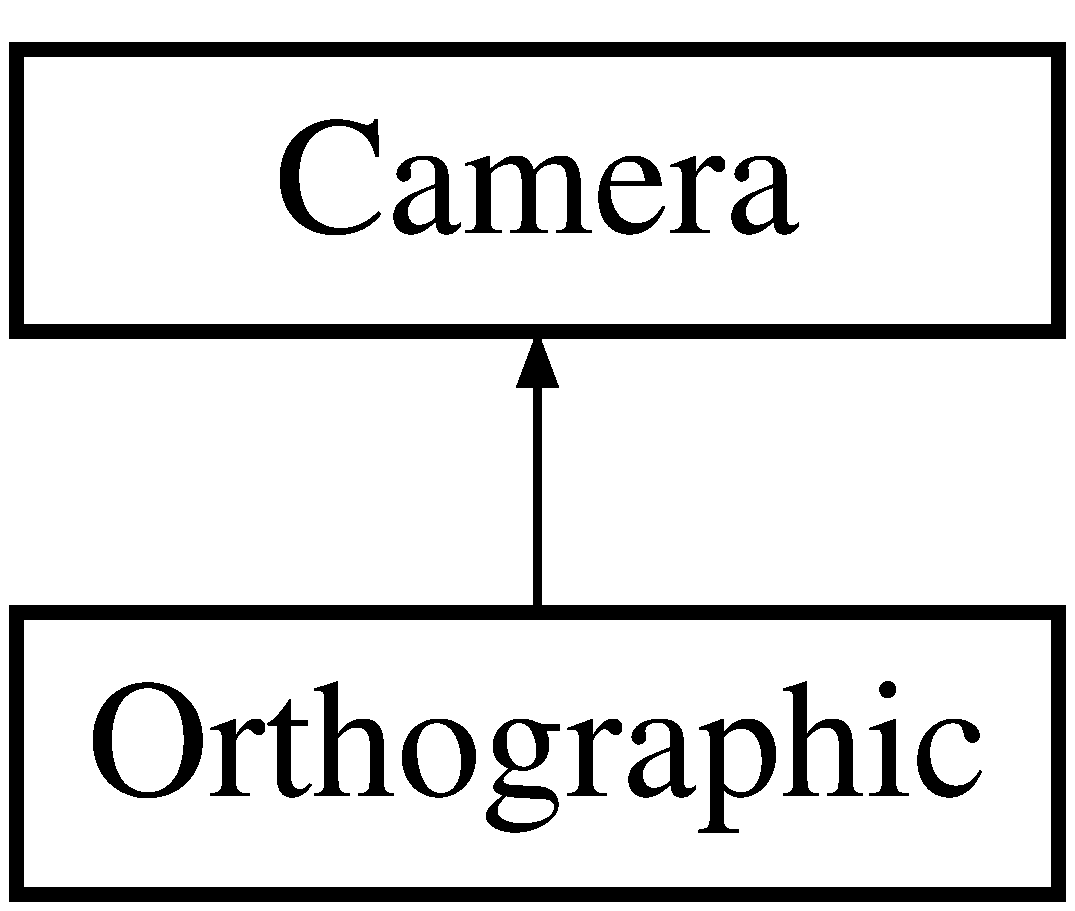
\includegraphics[height=2.000000cm]{class_orthographic}
\end{center}
\end{figure}
\subsection*{Public Member Functions}
\begin{DoxyCompactItemize}
\item 
\hyperlink{class_orthographic_a3b6a0b737a8f9d8b3c1961241aef04dc}{Orthographic} ()
\item 
virtual void \hyperlink{class_orthographic_a0d7ee7bfe619febed73725b99d2cc0b0}{Render\+Scene} (const World \&w)
\item 
void \hyperlink{group___cameras_ga4ad79de10c562075c049f2e580f48f9f}{Set\+View\+Plane\+Distance} (const float distance)
\item 
void \hyperlink{group___cameras_ga9a63b65c5228dc43caae0b986ea8d220}{Set\+Zoom} (const float zoom)
\end{DoxyCompactItemize}
\subsection*{Additional Inherited Members}


\subsection{Detailed Description}
A point from which the scene will be rendered with orthographic viewing. \begin{DoxyRemark}{Remarks}
T\+O\+DO. 
\end{DoxyRemark}


\subsection{Constructor \& Destructor Documentation}
\hypertarget{class_orthographic_a3b6a0b737a8f9d8b3c1961241aef04dc}{}\label{class_orthographic_a3b6a0b737a8f9d8b3c1961241aef04dc} 
\index{Orthographic@{Orthographic}!Orthographic@{Orthographic}}
\index{Orthographic@{Orthographic}!Orthographic@{Orthographic}}
\subsubsection{\texorpdfstring{Orthographic()}{Orthographic()}}
{\footnotesize\ttfamily Orthographic\+::\+Orthographic (\begin{DoxyParamCaption}{ }\end{DoxyParamCaption})}

Standard constructor. 

\subsection{Member Function Documentation}
\hypertarget{class_orthographic_a0d7ee7bfe619febed73725b99d2cc0b0}{}\label{class_orthographic_a0d7ee7bfe619febed73725b99d2cc0b0} 
\index{Orthographic@{Orthographic}!Render\+Scene@{Render\+Scene}}
\index{Render\+Scene@{Render\+Scene}!Orthographic@{Orthographic}}
\subsubsection{\texorpdfstring{Render\+Scene()}{RenderScene()}}
{\footnotesize\ttfamily virtual void Orthographic\+::\+Render\+Scene (\begin{DoxyParamCaption}\item[{const World \&}]{w }\end{DoxyParamCaption})\hspace{0.3cm}{\ttfamily [virtual]}}

Traces the constructed scene. 
\begin{DoxyParams}{Parameters}
{\em w} & Reference to the world. \\
\hline
\end{DoxyParams}


Implements \hyperlink{class_camera_ad65367e9b225387219d013ffed3f621a}{Camera}.



The documentation for this class was generated from the following file\+:\begin{DoxyCompactItemize}
\item 
Source/\+Cameras/include/\hyperlink{_orthographic_8h}{Orthographic.\+h}\end{DoxyCompactItemize}

\hypertarget{class_phong}{}\section{Phong Class Reference}
\label{class_phong}\index{Phong@{Phong}}


{\ttfamily \#include $<$Phong.\+h$>$}

Inheritance diagram for Phong\+:\begin{figure}[H]
\begin{center}
\leavevmode
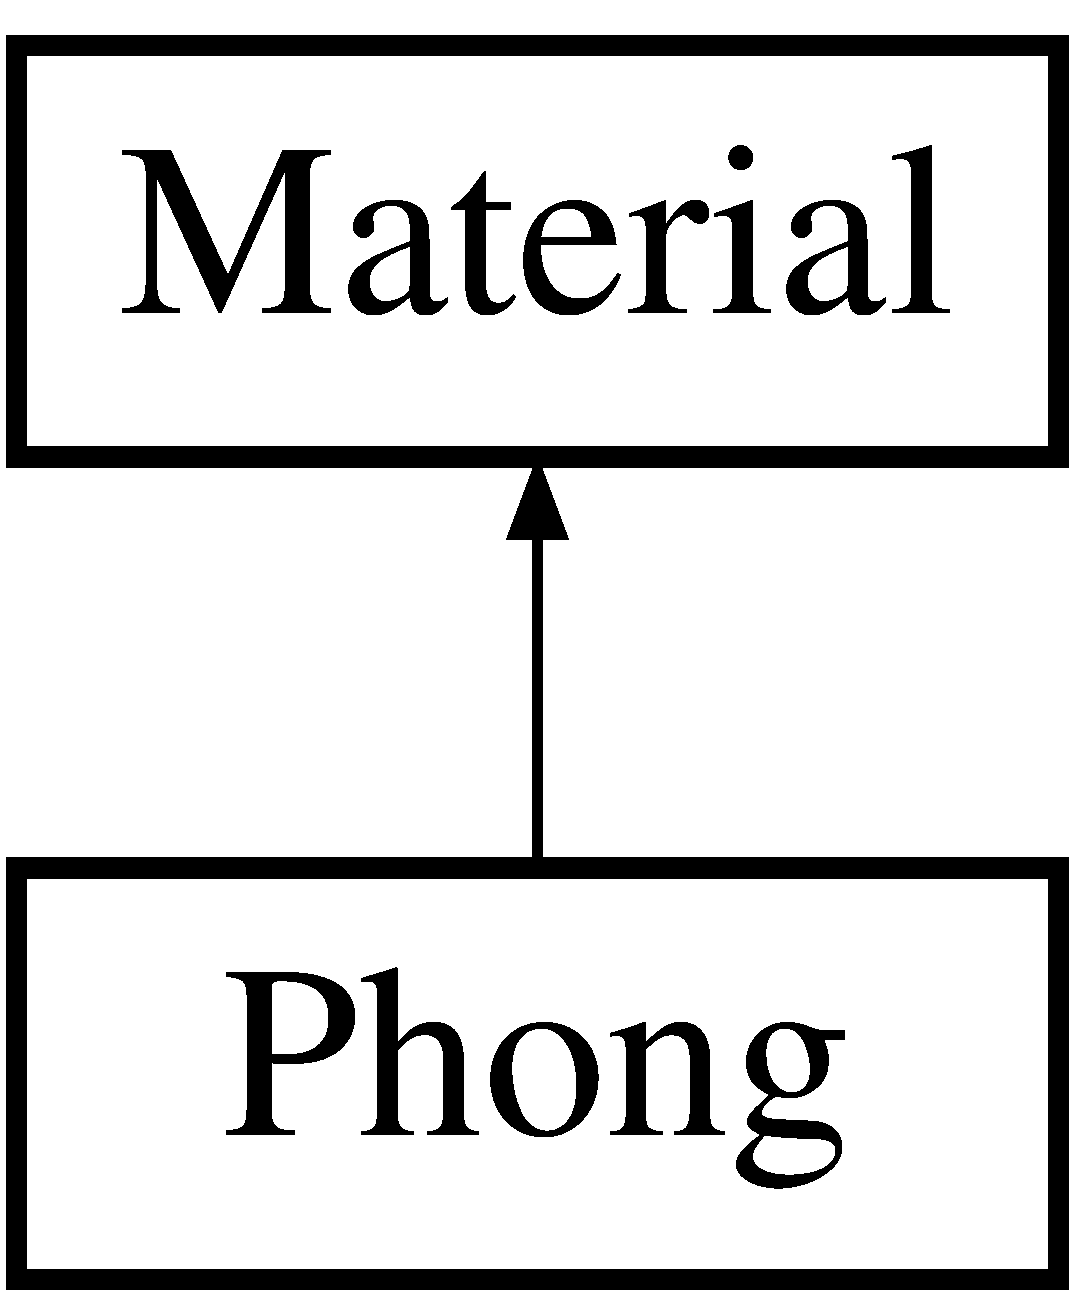
\includegraphics[height=2.000000cm]{class_phong}
\end{center}
\end{figure}
\subsection*{Public Member Functions}
\begin{DoxyCompactItemize}
\item 
\hyperlink{class_phong_a6b04845ec7a57cce73ee7d3355b0bf98}{Phong} ()
\item 
virtual \hyperlink{class_r_g_b_color}{R\+G\+B\+Color} \hyperlink{class_phong_a4ab7e1d4514c37abe47e18d627856dc8}{Shade} (\hyperlink{class_surface}{Surface} \&sr) const
\item 
void \hyperlink{group___materials_ga245b163a849cf378e84ed77620172f74}{Set\+Ambient\+Reflection} (const float kdr)
\item 
void \hyperlink{group___materials_ga7562b2e0139a3e2e93e61954d13c281f}{Set\+Ambient\+Color} (const \hyperlink{class_r_g_b_color}{R\+G\+B\+Color} \&color)
\item 
void \hyperlink{group___materials_ga7d9198210719a327b6c293955a9ecafe}{Set\+Diffuse\+Reflection} (const float kdr)
\item 
void \hyperlink{group___materials_ga54c0c1a1b40732588660aebbe01ce94f}{Set\+Diffuse\+Color} (const \hyperlink{class_r_g_b_color}{R\+G\+B\+Color} \&color)
\item 
void \hyperlink{group___materials_gaaa0823035fefb08e6f20e4af9c6f73d2}{Set\+Specular\+Reflection} (const float kdr)
\item 
void \hyperlink{group___materials_gaed8372d4e59cb7c1b781979c4ea9ee80}{Set\+Specular\+Color} (const \hyperlink{class_r_g_b_color}{R\+G\+B\+Color} \&color)
\item 
void \hyperlink{group___materials_ga167d70d514005d94a0bede7d7b12f372}{Set\+Specular\+Exponent} (const float ksexp)
\item 
void \hyperlink{group___materials_ga76b02c8e5a8dfff0a24c929b37a47c0c}{Set\+Sampler} (std\+::shared\+\_\+ptr$<$ \hyperlink{class_sampler}{Sampler} $>$)
\end{DoxyCompactItemize}


\subsection{Detailed Description}
Rendering properties of an object. \begin{DoxyRemark}{Remarks}
T\+O\+DO. 
\end{DoxyRemark}
\begin{DoxySeeAlso}{See also}
\hyperlink{class_lambertian}{Lambertian} 

\hyperlink{class_glossy_specular}{Glossy\+Specular} 
\end{DoxySeeAlso}


\subsection{Constructor \& Destructor Documentation}
\hypertarget{class_phong_a6b04845ec7a57cce73ee7d3355b0bf98}{}\label{class_phong_a6b04845ec7a57cce73ee7d3355b0bf98} 
\index{Phong@{Phong}!Phong@{Phong}}
\index{Phong@{Phong}!Phong@{Phong}}
\subsubsection{\texorpdfstring{Phong()}{Phong()}}
{\footnotesize\ttfamily Phong\+::\+Phong (\begin{DoxyParamCaption}{ }\end{DoxyParamCaption})}

Standard constructor. 

\subsection{Member Function Documentation}
\hypertarget{class_phong_a4ab7e1d4514c37abe47e18d627856dc8}{}\label{class_phong_a4ab7e1d4514c37abe47e18d627856dc8} 
\index{Phong@{Phong}!Shade@{Shade}}
\index{Shade@{Shade}!Phong@{Phong}}
\subsubsection{\texorpdfstring{Shade()}{Shade()}}
{\footnotesize\ttfamily virtual \hyperlink{class_r_g_b_color}{R\+G\+B\+Color} Phong\+::\+Shade (\begin{DoxyParamCaption}\item[{\hyperlink{class_surface}{Surface} \&}]{sr }\end{DoxyParamCaption}) const\hspace{0.3cm}{\ttfamily [virtual]}}

Computes the color of a given surface. 
\begin{DoxyParams}{Parameters}
{\em sr} & Information about the surface of the object. \\
\hline
\end{DoxyParams}
\begin{DoxyReturn}{Returns}
Color of the surface. 
\end{DoxyReturn}


Reimplemented from \hyperlink{class_material_aeccd880ee7b86a849e8f2d2f0bcf4fc7}{Material}.



The documentation for this class was generated from the following file\+:\begin{DoxyCompactItemize}
\item 
Source/\+Materials/include/\hyperlink{_phong_8h}{Phong.\+h}\end{DoxyCompactItemize}

\hypertarget{class_pinhole}{}\section{Pinhole Class Reference}
\label{class_pinhole}\index{Pinhole@{Pinhole}}


{\ttfamily \#include $<$Pinhole.\+h$>$}

Inheritance diagram for Pinhole\+:\begin{figure}[H]
\begin{center}
\leavevmode
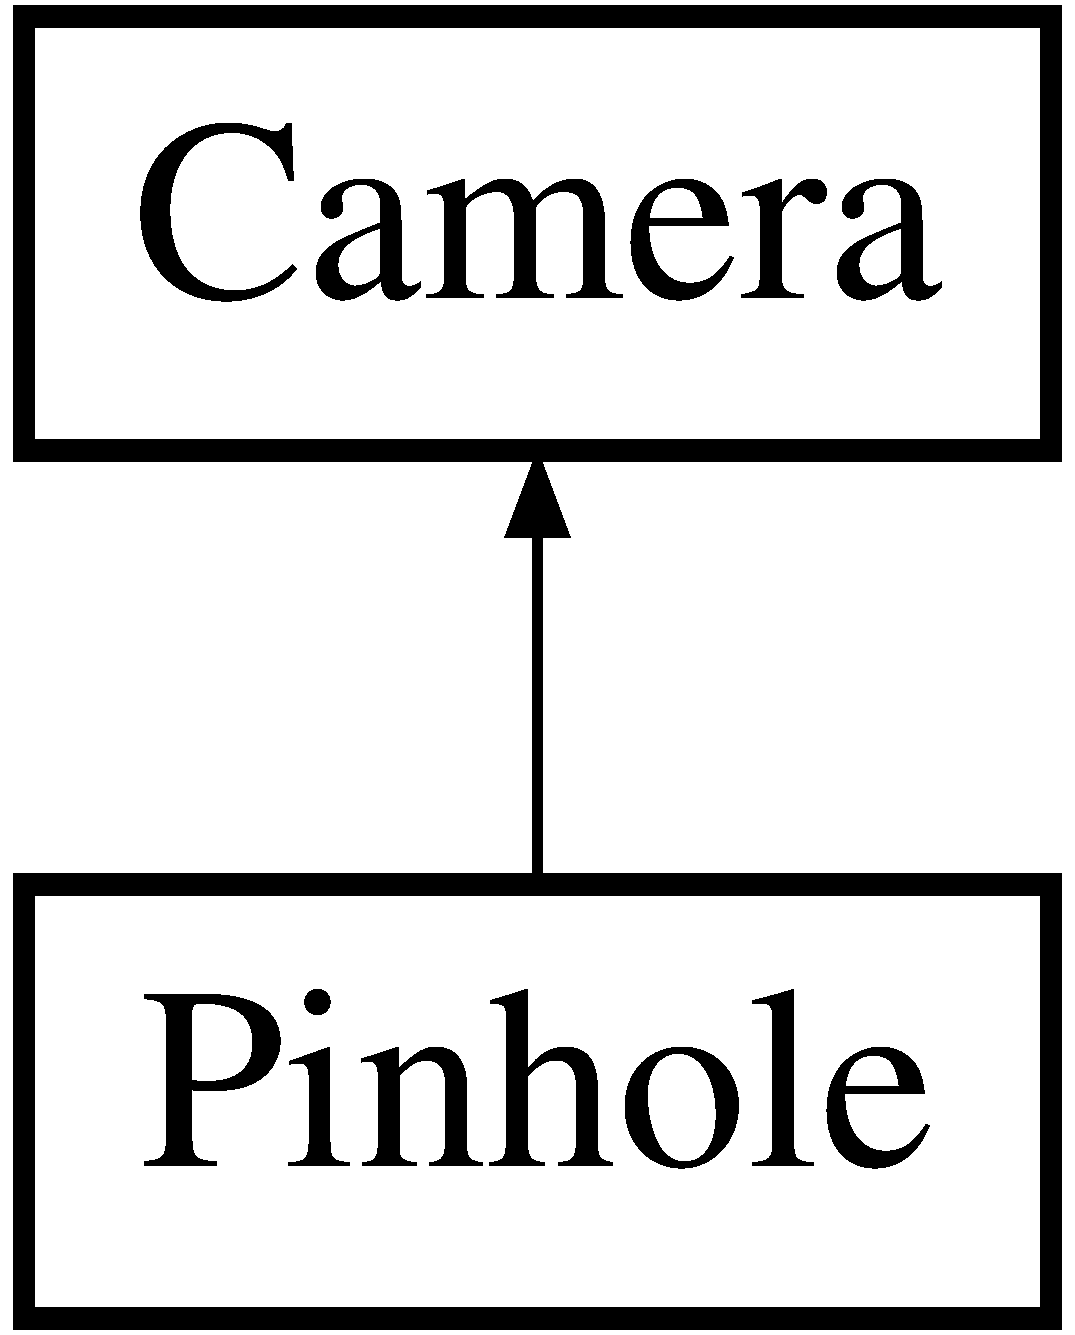
\includegraphics[height=2.000000cm]{class_pinhole}
\end{center}
\end{figure}
\subsection*{Public Member Functions}
\begin{DoxyCompactItemize}
\item 
\hyperlink{class_pinhole_aa106e56874db8211c2480096aff67051}{Pinhole} ()
\item 
virtual void \hyperlink{class_pinhole_a722af80f738cf4e8adba65926ffea9c9}{Render\+Scene} (const World \&w)
\item 
void \hyperlink{group___cameras_ga2757f00b8e8e778b6792b0c9e0e4052b}{Set\+View\+Plane\+Distance} (const float distance)
\item 
void \hyperlink{group___cameras_ga9baed583b61d1808867251fa33d4db56}{Set\+Zoom} (const float zoom)
\end{DoxyCompactItemize}
\subsection*{Additional Inherited Members}


\subsection{Detailed Description}
A point from which the scene will be rendered with perspective viewing. \begin{DoxyRemark}{Remarks}
T\+O\+DO. 
\end{DoxyRemark}


\subsection{Constructor \& Destructor Documentation}
\hypertarget{class_pinhole_aa106e56874db8211c2480096aff67051}{}\label{class_pinhole_aa106e56874db8211c2480096aff67051} 
\index{Pinhole@{Pinhole}!Pinhole@{Pinhole}}
\index{Pinhole@{Pinhole}!Pinhole@{Pinhole}}
\subsubsection{\texorpdfstring{Pinhole()}{Pinhole()}}
{\footnotesize\ttfamily Pinhole\+::\+Pinhole (\begin{DoxyParamCaption}{ }\end{DoxyParamCaption})}

Standard constructor. 

\subsection{Member Function Documentation}
\hypertarget{class_pinhole_a722af80f738cf4e8adba65926ffea9c9}{}\label{class_pinhole_a722af80f738cf4e8adba65926ffea9c9} 
\index{Pinhole@{Pinhole}!Render\+Scene@{Render\+Scene}}
\index{Render\+Scene@{Render\+Scene}!Pinhole@{Pinhole}}
\subsubsection{\texorpdfstring{Render\+Scene()}{RenderScene()}}
{\footnotesize\ttfamily virtual void Pinhole\+::\+Render\+Scene (\begin{DoxyParamCaption}\item[{const World \&}]{w }\end{DoxyParamCaption})\hspace{0.3cm}{\ttfamily [virtual]}}

Traces the constructed scene. 
\begin{DoxyParams}{Parameters}
{\em w} & Reference to the world. \\
\hline
\end{DoxyParams}


Implements \hyperlink{class_camera_ad65367e9b225387219d013ffed3f621a}{Camera}.



The documentation for this class was generated from the following file\+:\begin{DoxyCompactItemize}
\item 
Source/\+Cameras/include/\hyperlink{_pinhole_8h}{Pinhole.\+h}\end{DoxyCompactItemize}

\hypertarget{class_plane}{}\section{Plane Class Reference}
\label{class_plane}\index{Plane@{Plane}}


{\ttfamily \#include $<$Plane.\+h$>$}

Inheritance diagram for Plane\+:\begin{figure}[H]
\begin{center}
\leavevmode
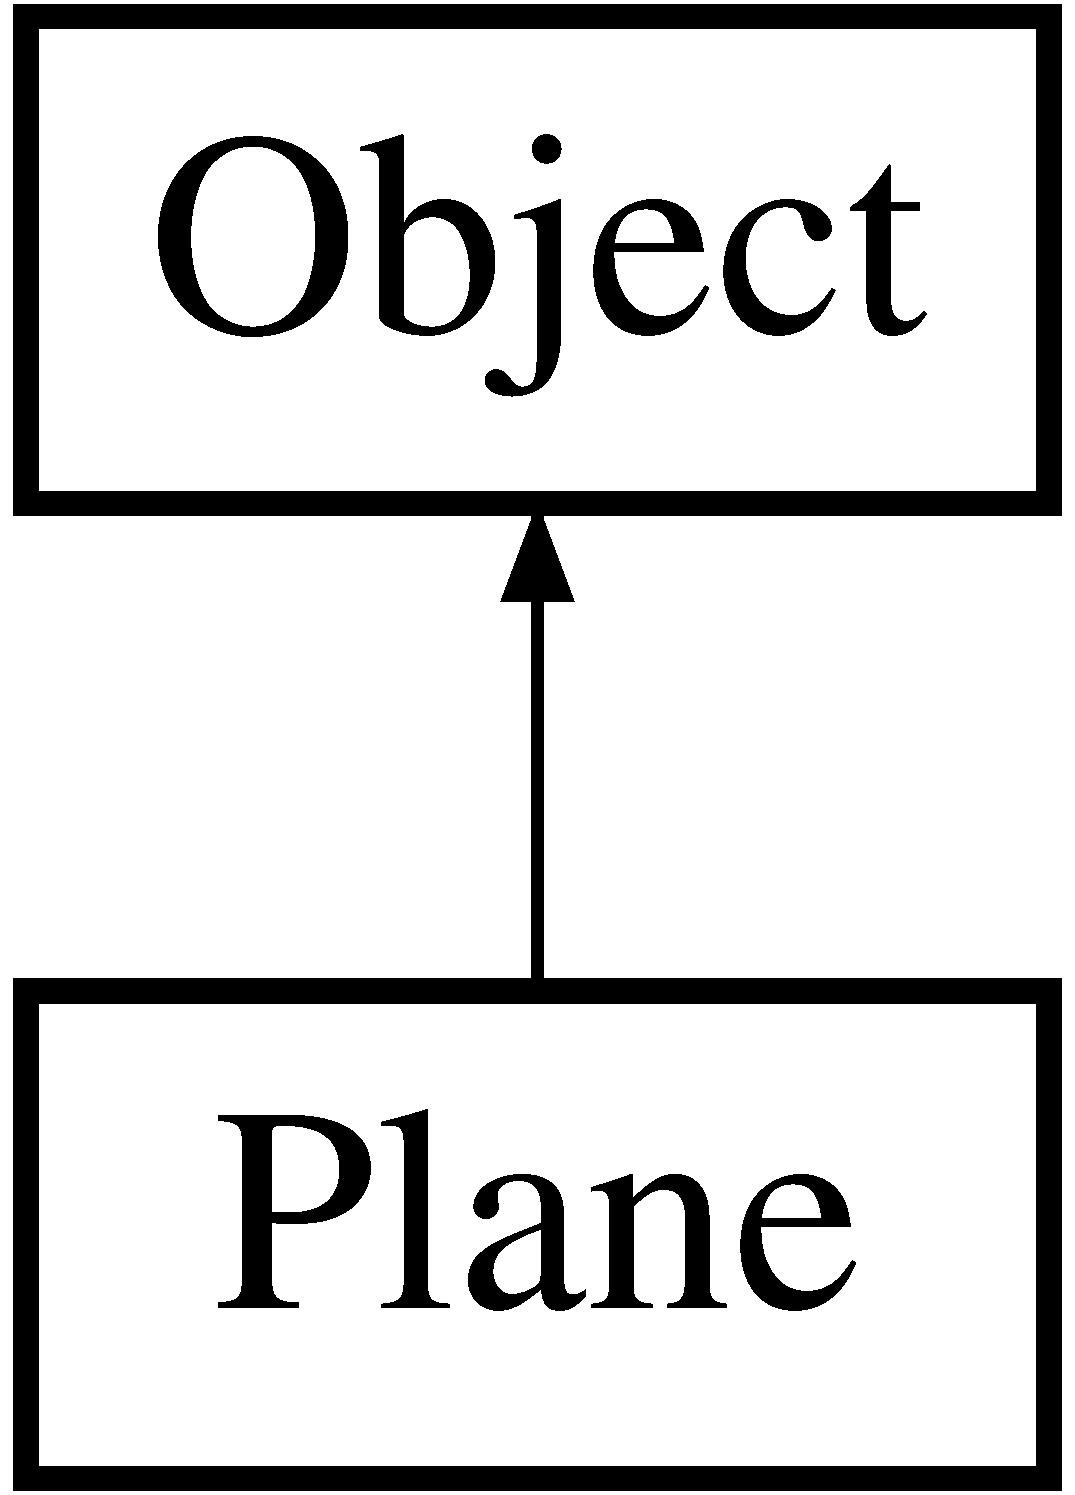
\includegraphics[height=2.000000cm]{class_plane}
\end{center}
\end{figure}
\subsection*{Public Member Functions}
\begin{DoxyCompactItemize}
\item 
\hyperlink{class_plane_acac0d9c003e0ab10d07b146c3566a0c7}{Plane} ()
\item 
virtual bool \hyperlink{class_plane_a71712655452a8ecbfe5907197e980c1e}{Hit} (const \hyperlink{class_ray}{Ray} \&ray, double \&tmin, \hyperlink{class_surface}{Surface} \&sr) const =0
\item 
virtual bool \hyperlink{class_plane_a21f6adf1c2be7853a61e1f8d811b76eb}{Shadow\+Hit} (const \hyperlink{class_ray}{Ray} \&ray, float \&tmin) const =0
\item 
void \hyperlink{group___geometric_objects_ga8fdaa0574a2046f2e280e6c926f7947d}{Set\+Point} (const glm\+::vec3 \&point)
\item 
void \hyperlink{group___geometric_objects_ga50e8800fa3595a6b6fafcda17a77388c}{Set\+Normal} (const glm\+::vec3 \&normal)
\end{DoxyCompactItemize}
\subsection*{Additional Inherited Members}


\subsection{Detailed Description}
Holder of data of a 3D plane. \begin{DoxyRemark}{Remarks}
T\+O\+DO. 
\end{DoxyRemark}


\subsection{Constructor \& Destructor Documentation}
\hypertarget{class_plane_acac0d9c003e0ab10d07b146c3566a0c7}{}\label{class_plane_acac0d9c003e0ab10d07b146c3566a0c7} 
\index{Plane@{Plane}!Plane@{Plane}}
\index{Plane@{Plane}!Plane@{Plane}}
\subsubsection{\texorpdfstring{Plane()}{Plane()}}
{\footnotesize\ttfamily Plane\+::\+Plane (\begin{DoxyParamCaption}{ }\end{DoxyParamCaption})}

Standard constructor. 

\subsection{Member Function Documentation}
\hypertarget{class_plane_a71712655452a8ecbfe5907197e980c1e}{}\label{class_plane_a71712655452a8ecbfe5907197e980c1e} 
\index{Plane@{Plane}!Hit@{Hit}}
\index{Hit@{Hit}!Plane@{Plane}}
\subsubsection{\texorpdfstring{Hit()}{Hit()}}
{\footnotesize\ttfamily virtual bool Plane\+::\+Hit (\begin{DoxyParamCaption}\item[{const \hyperlink{class_ray}{Ray} \&}]{ray,  }\item[{double \&}]{tmin,  }\item[{\hyperlink{class_surface}{Surface} \&}]{sr }\end{DoxyParamCaption}) const\hspace{0.3cm}{\ttfamily [pure virtual]}}

Checks if a ray intersects with this object and return it\textquotesingle{}s shading information. 
\begin{DoxyParams}{Parameters}
{\em ray} & Intersection ray. \\
\hline
{\em tmin} & T\+O\+DO. \\
\hline
{\em sr} & Information about the surface of the object. \\
\hline
\end{DoxyParams}
\begin{DoxyReturn}{Returns}
True, if the object intersects with the given ray. 
\end{DoxyReturn}


Implements \hyperlink{class_object_ad9977e40c0a3048eba9a81b25efcf3ef}{Object}.

\hypertarget{class_plane_a21f6adf1c2be7853a61e1f8d811b76eb}{}\label{class_plane_a21f6adf1c2be7853a61e1f8d811b76eb} 
\index{Plane@{Plane}!Shadow\+Hit@{Shadow\+Hit}}
\index{Shadow\+Hit@{Shadow\+Hit}!Plane@{Plane}}
\subsubsection{\texorpdfstring{Shadow\+Hit()}{ShadowHit()}}
{\footnotesize\ttfamily virtual bool Plane\+::\+Shadow\+Hit (\begin{DoxyParamCaption}\item[{const \hyperlink{class_ray}{Ray} \&}]{ray,  }\item[{float \&}]{tmin }\end{DoxyParamCaption}) const\hspace{0.3cm}{\ttfamily [pure virtual]}}

Checks if a shadow ray intersects with the object. 
\begin{DoxyParams}{Parameters}
{\em ray} & Shadow ray. \\
\hline
{\em tmin} & T\+O\+DO \\
\hline
\end{DoxyParams}
\begin{DoxyReturn}{Returns}
True, if the object intersects with the given ray. 
\end{DoxyReturn}


Implements \hyperlink{class_object_a020a6edbef7b2591b1dd6815ebbc5aa0}{Object}.



The documentation for this class was generated from the following file\+:\begin{DoxyCompactItemize}
\item 
Source/\+Geometric\+Objects/include/\hyperlink{_plane_8h}{Plane.\+h}\end{DoxyCompactItemize}

\hypertarget{class_point_light}{}\section{Point\+Light Class Reference}
\label{class_point_light}\index{Point\+Light@{Point\+Light}}


{\ttfamily \#include $<$Point\+Light.\+h$>$}

Inheritance diagram for Point\+Light\+:\begin{figure}[H]
\begin{center}
\leavevmode
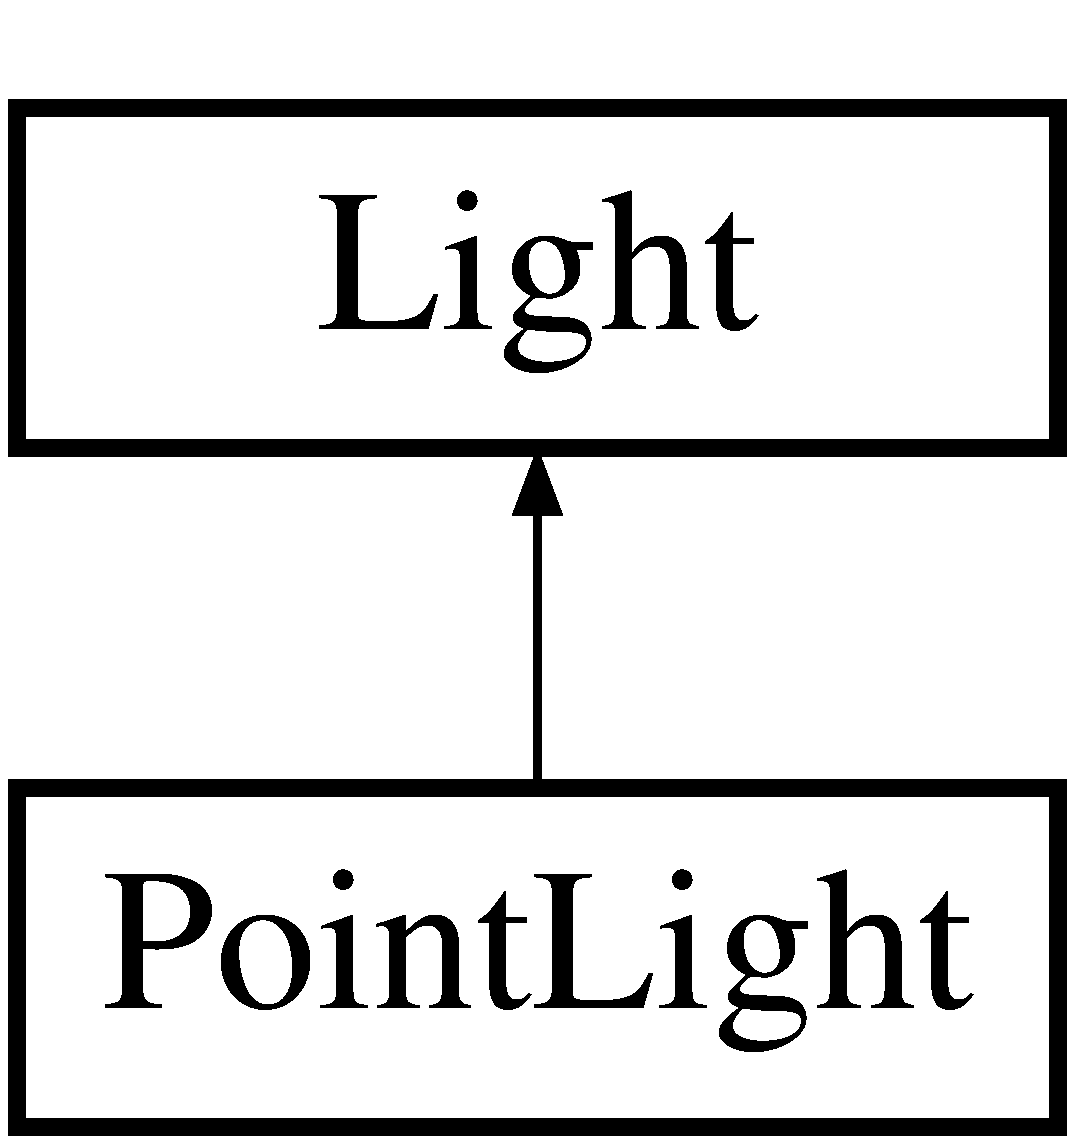
\includegraphics[height=2.000000cm]{class_point_light}
\end{center}
\end{figure}
\subsection*{Public Member Functions}
\begin{DoxyCompactItemize}
\item 
\hyperlink{class_point_light_abbfdf5f05b559c49016f8bb97b0ca414}{Point\+Light} ()
\item 
virtual glm\+::vec3 \hyperlink{class_point_light_af587fd5a2e72f32fcf5041a2cfb055e1}{Get\+Direction} (\hyperlink{class_surface}{Surface} \&sr)
\item 
virtual \hyperlink{class_r_g_b_color}{R\+G\+B\+Color} \hyperlink{class_point_light_a0d5e1227bc28f5a26edb595fe443f7f3}{L} (\hyperlink{class_surface}{Surface} \&sr)
\item 
virtual bool \hyperlink{class_point_light_aa4a50b149cdc22acbf2140a7e2ff9551}{Shadowed} (const \hyperlink{class_ray}{Ray} \&ray, const \hyperlink{class_surface}{Surface} \&sr) const
\item 
void \hyperlink{group___lights_ga1d97c3f6d636899b719d5014f74b3530}{Set\+Intensity} (const float intensity)
\item 
void \hyperlink{group___lights_ga27c17e299711f7131091c714b837f619}{Set\+Color} (const \hyperlink{class_r_g_b_color}{R\+G\+B\+Color} \&color)
\item 
void \hyperlink{group___lights_ga21b458bf745d4fe52a62e503a4fb3d24}{Set\+Position} (const glm\+::vec3 \&position)
\end{DoxyCompactItemize}
\subsection*{Additional Inherited Members}


\subsection{Detailed Description}
Representation of a point light source. \begin{DoxyRemark}{Remarks}
T\+O\+DO 
\end{DoxyRemark}


\subsection{Constructor \& Destructor Documentation}
\hypertarget{class_point_light_abbfdf5f05b559c49016f8bb97b0ca414}{}\label{class_point_light_abbfdf5f05b559c49016f8bb97b0ca414} 
\index{Point\+Light@{Point\+Light}!Point\+Light@{Point\+Light}}
\index{Point\+Light@{Point\+Light}!Point\+Light@{Point\+Light}}
\subsubsection{\texorpdfstring{Point\+Light()}{PointLight()}}
{\footnotesize\ttfamily Point\+Light\+::\+Point\+Light (\begin{DoxyParamCaption}{ }\end{DoxyParamCaption})}

Standard constructor. 

\subsection{Member Function Documentation}
\hypertarget{class_point_light_af587fd5a2e72f32fcf5041a2cfb055e1}{}\label{class_point_light_af587fd5a2e72f32fcf5041a2cfb055e1} 
\index{Point\+Light@{Point\+Light}!Get\+Direction@{Get\+Direction}}
\index{Get\+Direction@{Get\+Direction}!Point\+Light@{Point\+Light}}
\subsubsection{\texorpdfstring{Get\+Direction()}{GetDirection()}}
{\footnotesize\ttfamily virtual glm\+::vec3 Point\+Light\+::\+Get\+Direction (\begin{DoxyParamCaption}\item[{\hyperlink{class_surface}{Surface} \&}]{sr }\end{DoxyParamCaption})\hspace{0.3cm}{\ttfamily [virtual]}}

Computes the direction of the incoming light at a given surface. 
\begin{DoxyParams}{Parameters}
{\em sr} & Information about the surface of the object. \\
\hline
\end{DoxyParams}
\begin{DoxyReturn}{Returns}
Direction from which the light arrives at the surface. 
\end{DoxyReturn}


Implements \hyperlink{class_light_a62c5f73131ca1cdd6b2477f36c242482}{Light}.

\hypertarget{class_point_light_a0d5e1227bc28f5a26edb595fe443f7f3}{}\label{class_point_light_a0d5e1227bc28f5a26edb595fe443f7f3} 
\index{Point\+Light@{Point\+Light}!L@{L}}
\index{L@{L}!Point\+Light@{Point\+Light}}
\subsubsection{\texorpdfstring{L()}{L()}}
{\footnotesize\ttfamily virtual \hyperlink{class_r_g_b_color}{R\+G\+B\+Color} Point\+Light\+::L (\begin{DoxyParamCaption}\item[{\hyperlink{class_surface}{Surface} \&}]{sr }\end{DoxyParamCaption})\hspace{0.3cm}{\ttfamily [virtual]}}

Computes the incident radiance at a given surface. 
\begin{DoxyParams}{Parameters}
{\em sr} & Information about the surface of the object. \\
\hline
\end{DoxyParams}
\begin{DoxyReturn}{Returns}
Incident radiance at the surface. 
\end{DoxyReturn}


Reimplemented from \hyperlink{class_light_aba4ca1dcd52876cb5bee71ac8f684af5}{Light}.

\hypertarget{class_point_light_aa4a50b149cdc22acbf2140a7e2ff9551}{}\label{class_point_light_aa4a50b149cdc22acbf2140a7e2ff9551} 
\index{Point\+Light@{Point\+Light}!Shadowed@{Shadowed}}
\index{Shadowed@{Shadowed}!Point\+Light@{Point\+Light}}
\subsubsection{\texorpdfstring{Shadowed()}{Shadowed()}}
{\footnotesize\ttfamily virtual bool Point\+Light\+::\+Shadowed (\begin{DoxyParamCaption}\item[{const \hyperlink{class_ray}{Ray} \&}]{ray,  }\item[{const \hyperlink{class_surface}{Surface} \&}]{sr }\end{DoxyParamCaption}) const\hspace{0.3cm}{\ttfamily [virtual]}}

Checks if a surface is shadowed by another object. 
\begin{DoxyParams}{Parameters}
{\em ray} & Casted shadow ray. \\
\hline
{\em sr} & Information about the surface of the object. \\
\hline
\end{DoxyParams}
\begin{DoxyReturn}{Returns}
True, if the surface is shadowed. 
\end{DoxyReturn}


Implements \hyperlink{class_light_ac96c5efcdccb339609c7d19ea6ac5d17}{Light}.



The documentation for this class was generated from the following file\+:\begin{DoxyCompactItemize}
\item 
Source/\+Lights/include/\hyperlink{_point_light_8h}{Point\+Light.\+h}\end{DoxyCompactItemize}

\hypertarget{class_pure_random}{}\section{Pure\+Random Class Reference}
\label{class_pure_random}\index{Pure\+Random@{Pure\+Random}}


{\ttfamily \#include $<$Pure\+Random.\+h$>$}

Inheritance diagram for Pure\+Random\+:\begin{figure}[H]
\begin{center}
\leavevmode
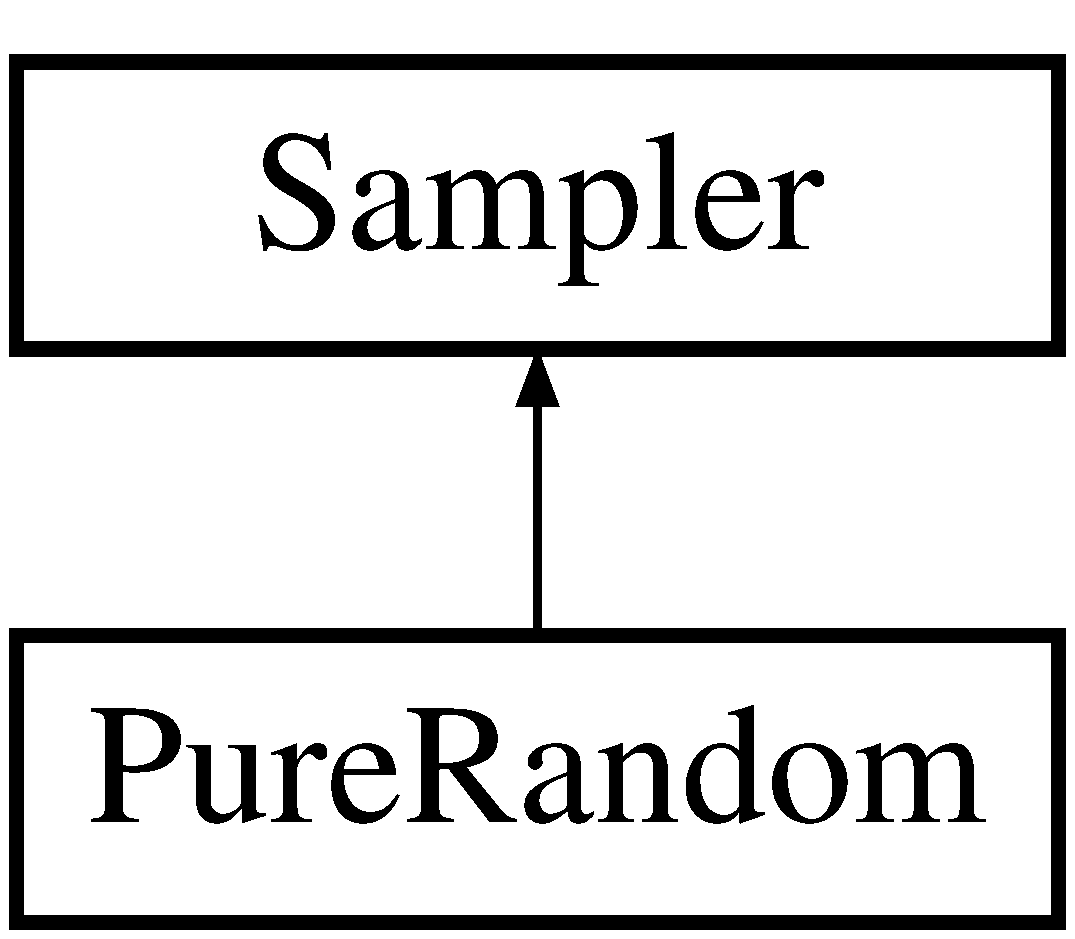
\includegraphics[height=2.000000cm]{class_pure_random}
\end{center}
\end{figure}
\subsection*{Public Member Functions}
\begin{DoxyCompactItemize}
\item 
\hyperlink{class_pure_random_a61f8ed0fdd5f477c4617b29460fac5e3}{Pure\+Random} ()
\item 
\hyperlink{class_pure_random_a071f6a64e2019dcf303365827707f490}{Pure\+Random} (const int num\+Samples)
\item 
\hyperlink{class_pure_random_a32af40bab93939c82bbd59605d5396bd}{Pure\+Random} (const int num\+Samples, const int num\+Sets)
\end{DoxyCompactItemize}
\subsection*{Additional Inherited Members}


\subsection{Detailed Description}
T\+O\+DO \begin{DoxyRemark}{Remarks}
T\+O\+DO. 
\end{DoxyRemark}


\subsection{Constructor \& Destructor Documentation}
\hypertarget{class_pure_random_a61f8ed0fdd5f477c4617b29460fac5e3}{}\label{class_pure_random_a61f8ed0fdd5f477c4617b29460fac5e3} 
\index{Pure\+Random@{Pure\+Random}!Pure\+Random@{Pure\+Random}}
\index{Pure\+Random@{Pure\+Random}!Pure\+Random@{Pure\+Random}}
\subsubsection{\texorpdfstring{Pure\+Random()}{PureRandom()}\hspace{0.1cm}{\footnotesize\ttfamily [1/3]}}
{\footnotesize\ttfamily Pure\+Random\+::\+Pure\+Random (\begin{DoxyParamCaption}{ }\end{DoxyParamCaption})}

Standard constructor. \hypertarget{class_pure_random_a071f6a64e2019dcf303365827707f490}{}\label{class_pure_random_a071f6a64e2019dcf303365827707f490} 
\index{Pure\+Random@{Pure\+Random}!Pure\+Random@{Pure\+Random}}
\index{Pure\+Random@{Pure\+Random}!Pure\+Random@{Pure\+Random}}
\subsubsection{\texorpdfstring{Pure\+Random()}{PureRandom()}\hspace{0.1cm}{\footnotesize\ttfamily [2/3]}}
{\footnotesize\ttfamily Pure\+Random\+::\+Pure\+Random (\begin{DoxyParamCaption}\item[{const int}]{num\+Samples }\end{DoxyParamCaption})}

Constructs a sampler and sets its number of samples. 
\begin{DoxyParams}{Parameters}
{\em num\+Samples} & Number of samples. \\
\hline
\end{DoxyParams}
\hypertarget{class_pure_random_a32af40bab93939c82bbd59605d5396bd}{}\label{class_pure_random_a32af40bab93939c82bbd59605d5396bd} 
\index{Pure\+Random@{Pure\+Random}!Pure\+Random@{Pure\+Random}}
\index{Pure\+Random@{Pure\+Random}!Pure\+Random@{Pure\+Random}}
\subsubsection{\texorpdfstring{Pure\+Random()}{PureRandom()}\hspace{0.1cm}{\footnotesize\ttfamily [3/3]}}
{\footnotesize\ttfamily Pure\+Random\+::\+Pure\+Random (\begin{DoxyParamCaption}\item[{const int}]{num\+Samples,  }\item[{const int}]{num\+Sets }\end{DoxyParamCaption})}

Constructs a sampler and sets its number of samples and sets. 
\begin{DoxyParams}{Parameters}
{\em num\+Samples} & Number of samples. \\
\hline
{\em num\+Sets} & Number of sets. \\
\hline
\end{DoxyParams}


The documentation for this class was generated from the following file\+:\begin{DoxyCompactItemize}
\item 
Source/\+Samplers/include/\hyperlink{_pure_random_8h}{Pure\+Random.\+h}\end{DoxyCompactItemize}

\hypertarget{class_ray}{}\section{Ray Class Reference}
\label{class_ray}\index{Ray@{Ray}}


{\ttfamily \#include $<$Ray.\+h$>$}

\subsection*{Public Member Functions}
\begin{DoxyCompactItemize}
\item 
\hyperlink{class_ray_a2e3d2c29f2df4ab3da10da79d4acb852}{Ray} ()
\item 
\hyperlink{class_ray_ae5670c390428ae21b8066329d87e1ad9}{Ray} (glm\+::vec3 \&origin, glm\+::vec3 \&direction)
\end{DoxyCompactItemize}
\subsection*{Public Attributes}
\begin{DoxyCompactItemize}
\item 
glm\+::vec3 \hyperlink{class_ray_ab94919c6ebaa2fd3628d8bc85669e79a}{m\+\_\+\+Origin}
\item 
glm\+::vec3 \hyperlink{class_ray_a1fe0679dfa9ead77bf81d4c7a8b87175}{m\+\_\+\+Direction}
\end{DoxyCompactItemize}


\subsection{Detailed Description}
\hyperlink{class_object}{Object} used to trace scenes. \begin{DoxyRemark}{Remarks}
T\+O\+DO 
\end{DoxyRemark}


\subsection{Constructor \& Destructor Documentation}
\hypertarget{class_ray_a2e3d2c29f2df4ab3da10da79d4acb852}{}\label{class_ray_a2e3d2c29f2df4ab3da10da79d4acb852} 
\index{Ray@{Ray}!Ray@{Ray}}
\index{Ray@{Ray}!Ray@{Ray}}
\subsubsection{\texorpdfstring{Ray()}{Ray()}\hspace{0.1cm}{\footnotesize\ttfamily [1/2]}}
{\footnotesize\ttfamily Ray\+::\+Ray (\begin{DoxyParamCaption}{ }\end{DoxyParamCaption})}

Standard constructor. \hypertarget{class_ray_ae5670c390428ae21b8066329d87e1ad9}{}\label{class_ray_ae5670c390428ae21b8066329d87e1ad9} 
\index{Ray@{Ray}!Ray@{Ray}}
\index{Ray@{Ray}!Ray@{Ray}}
\subsubsection{\texorpdfstring{Ray()}{Ray()}\hspace{0.1cm}{\footnotesize\ttfamily [2/2]}}
{\footnotesize\ttfamily Ray\+::\+Ray (\begin{DoxyParamCaption}\item[{glm\+::vec3 \&}]{origin,  }\item[{glm\+::vec3 \&}]{direction }\end{DoxyParamCaption})}

Constructs a ray with the target origin and direction. 
\begin{DoxyParams}{Parameters}
{\em origin} & Target origin. \\
\hline
{\em direction} & Target direction. \\
\hline
\end{DoxyParams}


\subsection{Member Data Documentation}
\hypertarget{class_ray_a1fe0679dfa9ead77bf81d4c7a8b87175}{}\label{class_ray_a1fe0679dfa9ead77bf81d4c7a8b87175} 
\index{Ray@{Ray}!m\+\_\+\+Direction@{m\+\_\+\+Direction}}
\index{m\+\_\+\+Direction@{m\+\_\+\+Direction}!Ray@{Ray}}
\subsubsection{\texorpdfstring{m\+\_\+\+Direction}{m\_Direction}}
{\footnotesize\ttfamily glm\+::vec3 Ray\+::m\+\_\+\+Direction}

Direction of the ray. \hypertarget{class_ray_ab94919c6ebaa2fd3628d8bc85669e79a}{}\label{class_ray_ab94919c6ebaa2fd3628d8bc85669e79a} 
\index{Ray@{Ray}!m\+\_\+\+Origin@{m\+\_\+\+Origin}}
\index{m\+\_\+\+Origin@{m\+\_\+\+Origin}!Ray@{Ray}}
\subsubsection{\texorpdfstring{m\+\_\+\+Origin}{m\_Origin}}
{\footnotesize\ttfamily glm\+::vec3 Ray\+::m\+\_\+\+Origin}

Origin of the ray in world coordinates. 

The documentation for this class was generated from the following file\+:\begin{DoxyCompactItemize}
\item 
Source/\+Utilities/include/\hyperlink{_ray_8h}{Ray.\+h}\end{DoxyCompactItemize}

\hypertarget{class_ray_cast}{}\section{Ray\+Cast Class Reference}
\label{class_ray_cast}\index{Ray\+Cast@{Ray\+Cast}}


{\ttfamily \#include $<$Ray\+Cast.\+h$>$}

Inheritance diagram for Ray\+Cast\+:\begin{figure}[H]
\begin{center}
\leavevmode
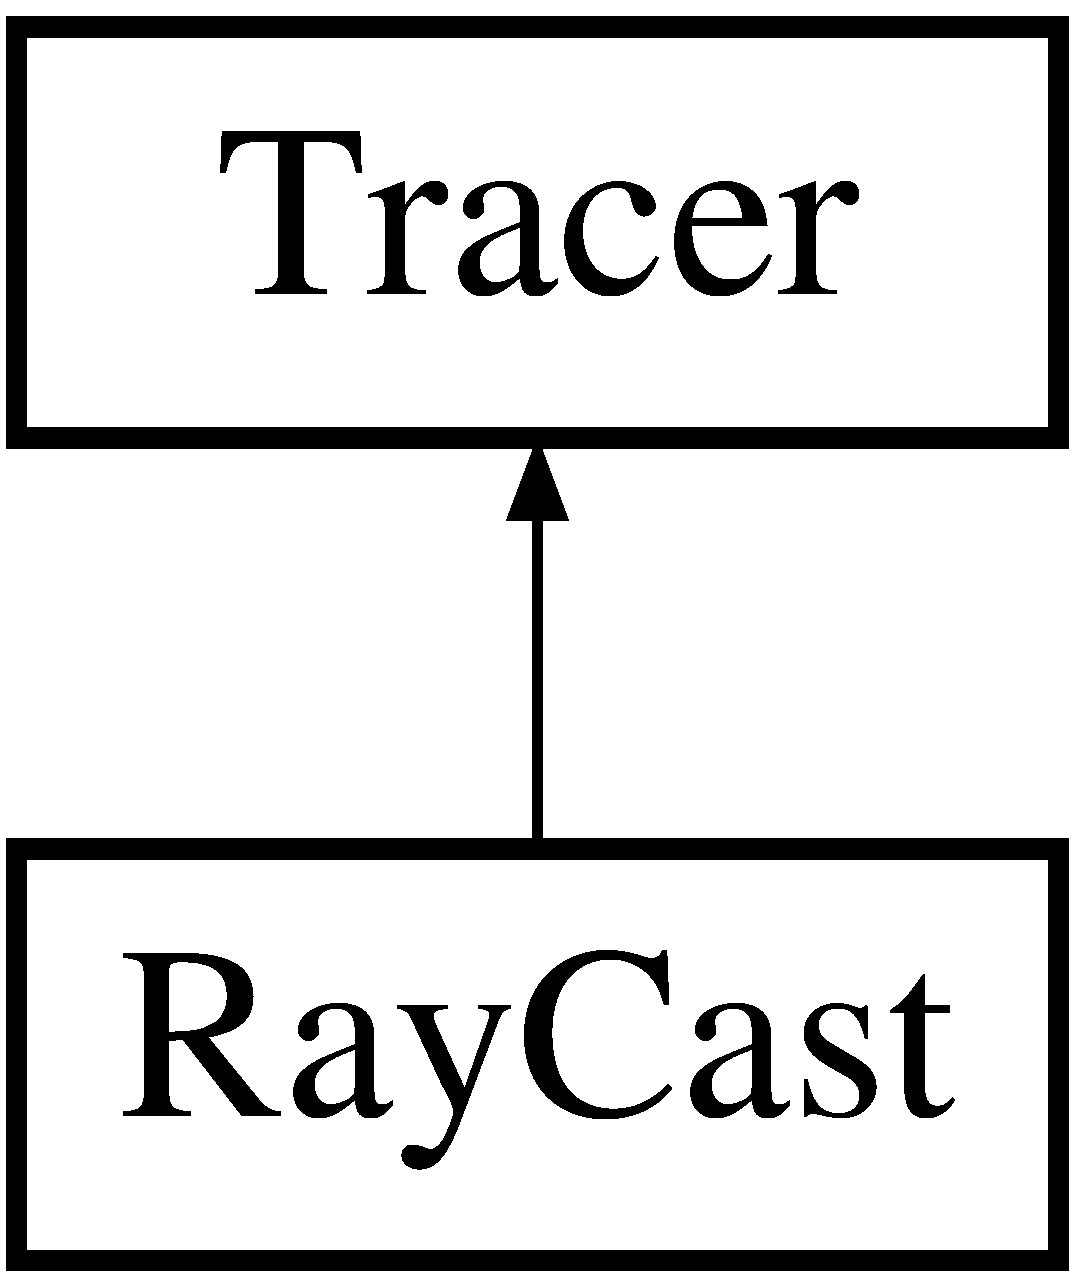
\includegraphics[height=2.000000cm]{class_ray_cast}
\end{center}
\end{figure}
\subsection*{Public Member Functions}
\begin{DoxyCompactItemize}
\item 
\hyperlink{class_ray_cast_adedb760a41eeb39a1ca797801727ae67}{Ray\+Cast} (std\+::shared\+\_\+ptr$<$ World $>$ world\+\_\+ptr)
\item 
virtual \hyperlink{class_r_g_b_color}{R\+G\+B\+Color} \hyperlink{class_ray_cast_aed24a822899e5328a7e668a479d3be9e}{Trace\+Ray} (const \hyperlink{class_ray}{Ray} \&ray) const
\end{DoxyCompactItemize}
\subsection*{Additional Inherited Members}


\subsection{Detailed Description}
T\+O\+DO. \begin{DoxyRemark}{Remarks}
T\+O\+DO. 
\end{DoxyRemark}


\subsection{Constructor \& Destructor Documentation}
\hypertarget{class_ray_cast_adedb760a41eeb39a1ca797801727ae67}{}\label{class_ray_cast_adedb760a41eeb39a1ca797801727ae67} 
\index{Ray\+Cast@{Ray\+Cast}!Ray\+Cast@{Ray\+Cast}}
\index{Ray\+Cast@{Ray\+Cast}!Ray\+Cast@{Ray\+Cast}}
\subsubsection{\texorpdfstring{Ray\+Cast()}{RayCast()}}
{\footnotesize\ttfamily Ray\+Cast\+::\+Ray\+Cast (\begin{DoxyParamCaption}\item[{std\+::shared\+\_\+ptr$<$ World $>$}]{world\+\_\+ptr }\end{DoxyParamCaption})}

Constructs a \hyperlink{class_tracer}{Tracer} with a pointer to the world. 
\begin{DoxyParams}{Parameters}
{\em world\+\_\+ptr} & Pointer to the world. \\
\hline
\end{DoxyParams}


\subsection{Member Function Documentation}
\hypertarget{class_ray_cast_aed24a822899e5328a7e668a479d3be9e}{}\label{class_ray_cast_aed24a822899e5328a7e668a479d3be9e} 
\index{Ray\+Cast@{Ray\+Cast}!Trace\+Ray@{Trace\+Ray}}
\index{Trace\+Ray@{Trace\+Ray}!Ray\+Cast@{Ray\+Cast}}
\subsubsection{\texorpdfstring{Trace\+Ray()}{TraceRay()}}
{\footnotesize\ttfamily virtual \hyperlink{class_r_g_b_color}{R\+G\+B\+Color} Ray\+Cast\+::\+Trace\+Ray (\begin{DoxyParamCaption}\item[{const \hyperlink{class_ray}{Ray} \&}]{ray }\end{DoxyParamCaption}) const\hspace{0.3cm}{\ttfamily [virtual]}}

Standard ray tracing method. 
\begin{DoxyParams}{Parameters}
{\em ray} & \hyperlink{class_ray}{Ray} traced. \\
\hline
\end{DoxyParams}
\begin{DoxyReturn}{Returns}
Color of the nearest surface hit by the ray. 
\end{DoxyReturn}


Reimplemented from \hyperlink{class_tracer_adbabdfde11e278945a0433d08445fcce}{Tracer}.



The documentation for this class was generated from the following file\+:\begin{DoxyCompactItemize}
\item 
Source/\+Tracers/include/\hyperlink{_ray_cast_8h}{Ray\+Cast.\+h}\end{DoxyCompactItemize}

\hypertarget{class_regular}{}\section{Regular Class Reference}
\label{class_regular}\index{Regular@{Regular}}


{\ttfamily \#include $<$Regular.\+h$>$}

Inheritance diagram for Regular\+:\begin{figure}[H]
\begin{center}
\leavevmode
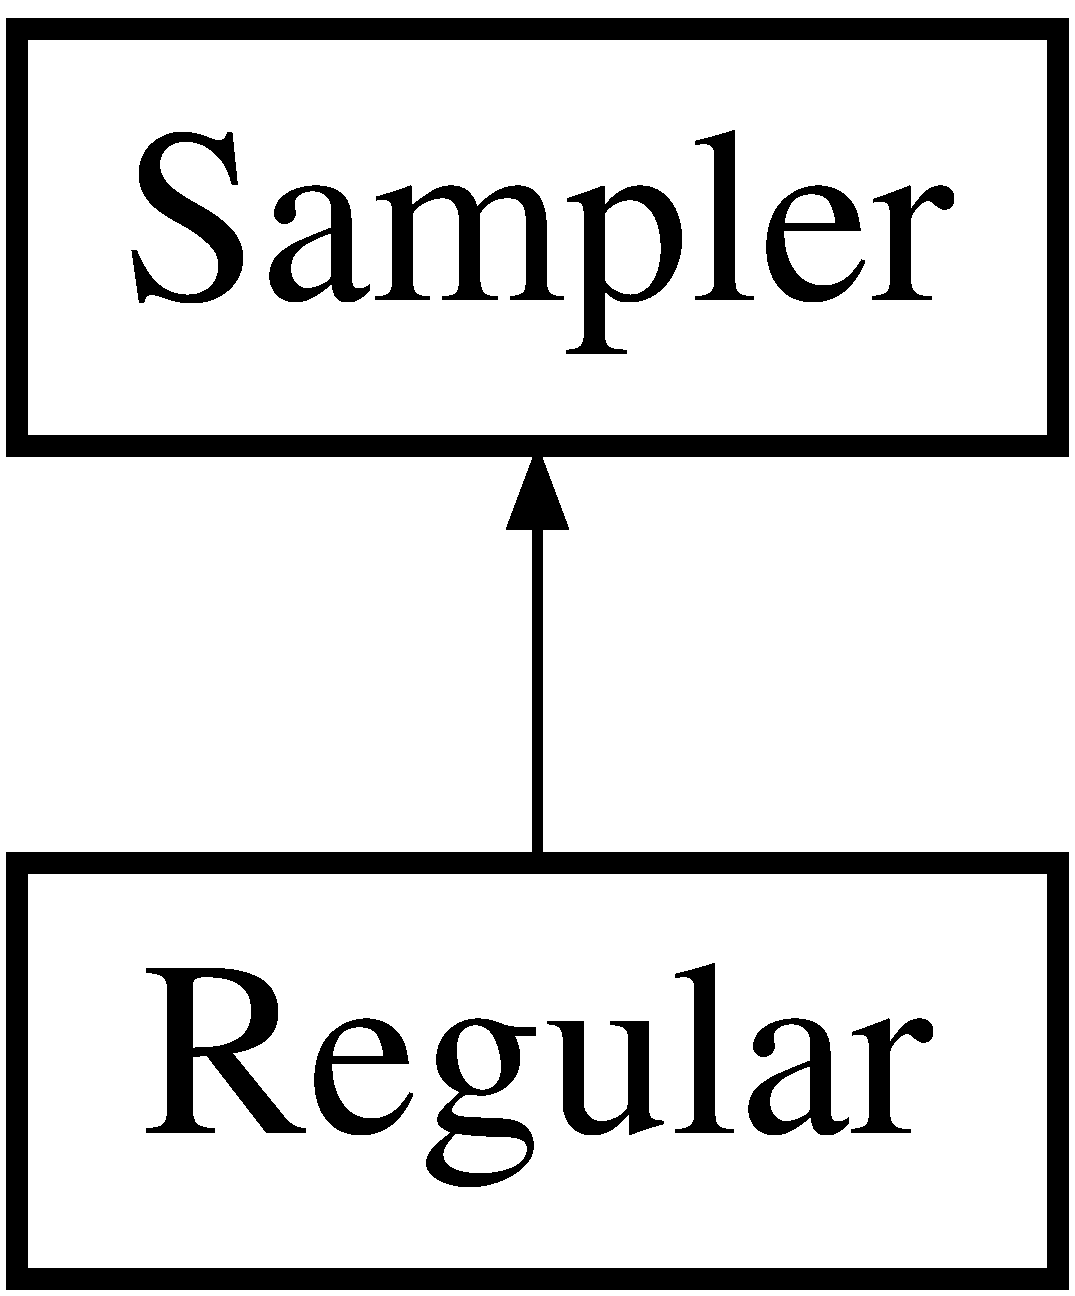
\includegraphics[height=2.000000cm]{class_regular}
\end{center}
\end{figure}
\subsection*{Public Member Functions}
\begin{DoxyCompactItemize}
\item 
\hyperlink{class_regular_ab37276a838198e8c3c14c6c0bd802a7b}{Regular} ()
\item 
\hyperlink{class_regular_a92a20b6c0adcd956b36c315a90eaff88}{Regular} (const int num\+Samples)
\item 
\hyperlink{class_regular_a2df0fa6fdfe2f6cf707677997486b395}{Regular} (const int num\+Samples, const int num\+Sets)
\end{DoxyCompactItemize}
\subsection*{Additional Inherited Members}


\subsection{Detailed Description}
T\+O\+DO \begin{DoxyRemark}{Remarks}
T\+O\+DO. 
\end{DoxyRemark}


\subsection{Constructor \& Destructor Documentation}
\hypertarget{class_regular_ab37276a838198e8c3c14c6c0bd802a7b}{}\label{class_regular_ab37276a838198e8c3c14c6c0bd802a7b} 
\index{Regular@{Regular}!Regular@{Regular}}
\index{Regular@{Regular}!Regular@{Regular}}
\subsubsection{\texorpdfstring{Regular()}{Regular()}\hspace{0.1cm}{\footnotesize\ttfamily [1/3]}}
{\footnotesize\ttfamily Regular\+::\+Regular (\begin{DoxyParamCaption}{ }\end{DoxyParamCaption})}

Standard constructor. \hypertarget{class_regular_a92a20b6c0adcd956b36c315a90eaff88}{}\label{class_regular_a92a20b6c0adcd956b36c315a90eaff88} 
\index{Regular@{Regular}!Regular@{Regular}}
\index{Regular@{Regular}!Regular@{Regular}}
\subsubsection{\texorpdfstring{Regular()}{Regular()}\hspace{0.1cm}{\footnotesize\ttfamily [2/3]}}
{\footnotesize\ttfamily Regular\+::\+Regular (\begin{DoxyParamCaption}\item[{const int}]{num\+Samples }\end{DoxyParamCaption})}

Constructs a sampler and sets its number of samples. 
\begin{DoxyParams}{Parameters}
{\em num\+Samples} & Number of samples. \\
\hline
\end{DoxyParams}
\hypertarget{class_regular_a2df0fa6fdfe2f6cf707677997486b395}{}\label{class_regular_a2df0fa6fdfe2f6cf707677997486b395} 
\index{Regular@{Regular}!Regular@{Regular}}
\index{Regular@{Regular}!Regular@{Regular}}
\subsubsection{\texorpdfstring{Regular()}{Regular()}\hspace{0.1cm}{\footnotesize\ttfamily [3/3]}}
{\footnotesize\ttfamily Regular\+::\+Regular (\begin{DoxyParamCaption}\item[{const int}]{num\+Samples,  }\item[{const int}]{num\+Sets }\end{DoxyParamCaption})}

Constructs a sampler and sets its number of samples and sets. 
\begin{DoxyParams}{Parameters}
{\em num\+Samples} & Number of samples. \\
\hline
{\em num\+Sets} & Number of sets. \\
\hline
\end{DoxyParams}


The documentation for this class was generated from the following file\+:\begin{DoxyCompactItemize}
\item 
Source/\+Samplers/include/\hyperlink{_regular_8h}{Regular.\+h}\end{DoxyCompactItemize}

\hypertarget{class_r_g_b_color}{}\section{R\+G\+B\+Color Class Reference}
\label{class_r_g_b_color}\index{R\+G\+B\+Color@{R\+G\+B\+Color}}


{\ttfamily \#include $<$R\+G\+B\+Color.\+h$>$}

\subsection*{Public Member Functions}
\begin{DoxyCompactItemize}
\item 
\hyperlink{class_r_g_b_color_a9383ce7b63b0a6ada5d4e54e16adf733}{R\+G\+B\+Color} ()
\item 
\hyperlink{class_r_g_b_color_a941e8548a929710ac1dc3b77ff5428d0}{R\+G\+B\+Color} (const float new\+\_\+r, const float new\+\_\+g, const float new\+\_\+b)
\item 
\hyperlink{class_r_g_b_color_a64e01e409f0db2a46a9c413c81c89d67}{R\+G\+B\+Color} (const float color)
\item 
bool \hyperlink{group___utilities_ga51f2ca82bd3166f19e7327c8e5e5a068}{operator==} (const \hyperlink{class_r_g_b_color}{R\+G\+B\+Color} \&rhs) const
\item 
\hyperlink{class_r_g_b_color}{R\+G\+B\+Color} \hyperlink{group___utilities_gab8eb3021ce94a9a4fc7a1ba1e8c06a30}{operator+} (const \hyperlink{class_r_g_b_color}{R\+G\+B\+Color} \&rhs) const
\item 
\hyperlink{class_r_g_b_color}{R\+G\+B\+Color} \hyperlink{group___utilities_ga2d0a70444ca0c882f3a5dbed42787ef8}{operator-\/} (const \hyperlink{class_r_g_b_color}{R\+G\+B\+Color} \&rhs) const
\item 
\hyperlink{class_r_g_b_color}{R\+G\+B\+Color} \hyperlink{group___utilities_ga38cb49925dc77a366b56b546b7dd17ae}{operator$\ast$} (const \hyperlink{class_r_g_b_color}{R\+G\+B\+Color} \&rhs) const
\item 
\hyperlink{class_r_g_b_color}{R\+G\+B\+Color} \hyperlink{group___utilities_ga46707b8ca0c4b560914f2aae4ec31eb5}{operator$\ast$} (const float rhs) const
\item 
\hyperlink{class_r_g_b_color}{R\+G\+B\+Color} \hyperlink{group___utilities_ga932f5821d1c40799b6b40f2fe88b7070}{operator/} (const float rhs) const
\item 
\hyperlink{class_r_g_b_color}{R\+G\+B\+Color} \hyperlink{group___utilities_ga985586cc676498527d1597ab3beee728}{operator+=} (const \hyperlink{class_r_g_b_color}{R\+G\+B\+Color} \&rhs)
\item 
\hyperlink{class_r_g_b_color}{R\+G\+B\+Color} \hyperlink{group___utilities_ga1a36960da5c88b5e3e825ad01845de29}{operator-\/=} (const \hyperlink{class_r_g_b_color}{R\+G\+B\+Color} \&rhs)
\item 
\hyperlink{class_r_g_b_color}{R\+G\+B\+Color} \hyperlink{class_r_g_b_color_a3a748bcc5393c391b8d7edb5dc162246}{operator$\ast$=} (const \hyperlink{class_r_g_b_color}{R\+G\+B\+Color} \&rhs)
\item 
\hyperlink{class_r_g_b_color}{R\+G\+B\+Color} \hyperlink{group___utilities_ga1b8ab73352d66c6d0125d6f061a1982f}{operator$\ast$=} (const float rhs)
\item 
\hyperlink{class_r_g_b_color}{R\+G\+B\+Color} \hyperlink{group___utilities_gad071890eadae01f96bf3af8ba52503e0}{operator/=} (const float rhs)
\item 
\hyperlink{class_r_g_b_color}{R\+G\+B\+Color} \hyperlink{class_r_g_b_color_a70f29cb9404fac9686687bc58efaaca2}{Pow} (const float exponent) const
\item 
float \hyperlink{group___utilities_gaea22cae2344d4a4187b50732820e50c8}{Average} () const
\end{DoxyCompactItemize}
\subsection*{Static Public Member Functions}
\begin{DoxyCompactItemize}
\item 
static \hyperlink{class_r_g_b_color}{R\+G\+B\+Color} \hyperlink{class_r_g_b_color_a767e650d2607d6a9138ab2929af21963}{Max\+To\+One} (const \hyperlink{class_r_g_b_color}{R\+G\+B\+Color} \&raw\+\_\+color)
\item 
static \hyperlink{class_r_g_b_color}{R\+G\+B\+Color} \hyperlink{class_r_g_b_color_acf9d559b664ee64da542949952bdf0f4}{Clamp\+To\+Color} (const \hyperlink{class_r_g_b_color}{R\+G\+B\+Color} \&raw\+\_\+color, const \hyperlink{class_r_g_b_color}{R\+G\+B\+Color} \&target\+\_\+color)
\end{DoxyCompactItemize}
\subsection*{Public Attributes}
\begin{DoxyCompactItemize}
\item 
float \hyperlink{class_r_g_b_color_a9c0b69a5100747dc0dee8d151129f8f2}{r}
\item 
float \hyperlink{class_r_g_b_color_a744b090c52455e09a4eacf55cabc39f9}{g}
\item 
float \hyperlink{class_r_g_b_color_adec4491768d446770055a6b23f18927d}{b}
\end{DoxyCompactItemize}
\subsection*{Static Public Attributes}
\begin{DoxyCompactItemize}
\item 
static const \hyperlink{class_r_g_b_color}{R\+G\+B\+Color} \hyperlink{class_r_g_b_color_a72f06dff766cb98998ef01f7018e1218}{Black}
\item 
static const \hyperlink{class_r_g_b_color}{R\+G\+B\+Color} \hyperlink{class_r_g_b_color_a2de4286a7090037773a2f3cd98685486}{White}
\item 
static const \hyperlink{class_r_g_b_color}{R\+G\+B\+Color} \hyperlink{class_r_g_b_color_a200488d3a3adcd67b66c452973f18c75}{Red}
\item 
static const \hyperlink{class_r_g_b_color}{R\+G\+B\+Color} \hyperlink{class_r_g_b_color_afaabce4b28b3e9306271830bebdfc7ab}{Green}
\item 
static const \hyperlink{class_r_g_b_color}{R\+G\+B\+Color} \hyperlink{class_r_g_b_color_a65d9d43015d92b2aab0d850bb73534db}{Blue}
\end{DoxyCompactItemize}


\subsection{Detailed Description}
Handles color channels and operations. \begin{DoxyRemark}{Remarks}
T\+O\+DO 
\end{DoxyRemark}


\subsection{Constructor \& Destructor Documentation}
\hypertarget{class_r_g_b_color_a9383ce7b63b0a6ada5d4e54e16adf733}{}\label{class_r_g_b_color_a9383ce7b63b0a6ada5d4e54e16adf733} 
\index{R\+G\+B\+Color@{R\+G\+B\+Color}!R\+G\+B\+Color@{R\+G\+B\+Color}}
\index{R\+G\+B\+Color@{R\+G\+B\+Color}!R\+G\+B\+Color@{R\+G\+B\+Color}}
\subsubsection{\texorpdfstring{R\+G\+B\+Color()}{RGBColor()}\hspace{0.1cm}{\footnotesize\ttfamily [1/3]}}
{\footnotesize\ttfamily R\+G\+B\+Color\+::\+R\+G\+B\+Color (\begin{DoxyParamCaption}{ }\end{DoxyParamCaption})}

Standard constructor. \hypertarget{class_r_g_b_color_a941e8548a929710ac1dc3b77ff5428d0}{}\label{class_r_g_b_color_a941e8548a929710ac1dc3b77ff5428d0} 
\index{R\+G\+B\+Color@{R\+G\+B\+Color}!R\+G\+B\+Color@{R\+G\+B\+Color}}
\index{R\+G\+B\+Color@{R\+G\+B\+Color}!R\+G\+B\+Color@{R\+G\+B\+Color}}
\subsubsection{\texorpdfstring{R\+G\+B\+Color()}{RGBColor()}\hspace{0.1cm}{\footnotesize\ttfamily [2/3]}}
{\footnotesize\ttfamily R\+G\+B\+Color\+::\+R\+G\+B\+Color (\begin{DoxyParamCaption}\item[{const float}]{new\+\_\+r,  }\item[{const float}]{new\+\_\+g,  }\item[{const float}]{new\+\_\+b }\end{DoxyParamCaption})}

Constructs an \hyperlink{class_r_g_b_color}{R\+G\+B\+Color} with the target components. 
\begin{DoxyParams}{Parameters}
{\em new\+\_\+r} & Target red component. \\
\hline
{\em new\+\_\+g} & Target green component. \\
\hline
{\em new\+\_\+b} & Target blue component. \\
\hline
\end{DoxyParams}
\hypertarget{class_r_g_b_color_a64e01e409f0db2a46a9c413c81c89d67}{}\label{class_r_g_b_color_a64e01e409f0db2a46a9c413c81c89d67} 
\index{R\+G\+B\+Color@{R\+G\+B\+Color}!R\+G\+B\+Color@{R\+G\+B\+Color}}
\index{R\+G\+B\+Color@{R\+G\+B\+Color}!R\+G\+B\+Color@{R\+G\+B\+Color}}
\subsubsection{\texorpdfstring{R\+G\+B\+Color()}{RGBColor()}\hspace{0.1cm}{\footnotesize\ttfamily [3/3]}}
{\footnotesize\ttfamily R\+G\+B\+Color\+::\+R\+G\+B\+Color (\begin{DoxyParamCaption}\item[{const float}]{color }\end{DoxyParamCaption})}

Constructs an \hyperlink{class_r_g_b_color}{R\+G\+B\+Color} with the target in all components. 
\begin{DoxyParams}{Parameters}
{\em color} & Target component. \\
\hline
\end{DoxyParams}


\subsection{Member Function Documentation}
\hypertarget{class_r_g_b_color_acf9d559b664ee64da542949952bdf0f4}{}\label{class_r_g_b_color_acf9d559b664ee64da542949952bdf0f4} 
\index{R\+G\+B\+Color@{R\+G\+B\+Color}!Clamp\+To\+Color@{Clamp\+To\+Color}}
\index{Clamp\+To\+Color@{Clamp\+To\+Color}!R\+G\+B\+Color@{R\+G\+B\+Color}}
\subsubsection{\texorpdfstring{Clamp\+To\+Color()}{ClampToColor()}}
{\footnotesize\ttfamily static \hyperlink{class_r_g_b_color}{R\+G\+B\+Color} R\+G\+B\+Color\+::\+Clamp\+To\+Color (\begin{DoxyParamCaption}\item[{const \hyperlink{class_r_g_b_color}{R\+G\+B\+Color} \&}]{raw\+\_\+color,  }\item[{const \hyperlink{class_r_g_b_color}{R\+G\+B\+Color} \&}]{target\+\_\+color }\end{DoxyParamCaption})\hspace{0.3cm}{\ttfamily [static]}}

Handles overflow of the color channel by mapping the out-\/of-\/gamut component to a target color. 
\begin{DoxyParams}{Parameters}
{\em raw\+\_\+color} & Out-\/of-\/gamut color. \\
\hline
{\em target\+\_\+color} & Target color. \\
\hline
\end{DoxyParams}
\begin{DoxyReturn}{Returns}
The campled color within the correct range with any overflow mapped to the target color. 
\end{DoxyReturn}
\hypertarget{class_r_g_b_color_a767e650d2607d6a9138ab2929af21963}{}\label{class_r_g_b_color_a767e650d2607d6a9138ab2929af21963} 
\index{R\+G\+B\+Color@{R\+G\+B\+Color}!Max\+To\+One@{Max\+To\+One}}
\index{Max\+To\+One@{Max\+To\+One}!R\+G\+B\+Color@{R\+G\+B\+Color}}
\subsubsection{\texorpdfstring{Max\+To\+One()}{MaxToOne()}}
{\footnotesize\ttfamily static \hyperlink{class_r_g_b_color}{R\+G\+B\+Color} R\+G\+B\+Color\+::\+Max\+To\+One (\begin{DoxyParamCaption}\item[{const \hyperlink{class_r_g_b_color}{R\+G\+B\+Color} \&}]{raw\+\_\+color }\end{DoxyParamCaption})\hspace{0.3cm}{\ttfamily [static]}}

Handles overflow of the color channel by dividing all the components by the out-\/of-\/gamut component. 
\begin{DoxyParams}{Parameters}
{\em raw\+\_\+color} & Out-\/of-\/gamut color. \\
\hline
\end{DoxyParams}
\begin{DoxyReturn}{Returns}
The clamped color within the correct range. 
\end{DoxyReturn}
\hypertarget{class_r_g_b_color_a3a748bcc5393c391b8d7edb5dc162246}{}\label{class_r_g_b_color_a3a748bcc5393c391b8d7edb5dc162246} 
\index{R\+G\+B\+Color@{R\+G\+B\+Color}!operator$\ast$=@{operator$\ast$=}}
\index{operator$\ast$=@{operator$\ast$=}!R\+G\+B\+Color@{R\+G\+B\+Color}}
\subsubsection{\texorpdfstring{operator$\ast$=()}{operator*=()}}
{\footnotesize\ttfamily \hyperlink{class_r_g_b_color}{R\+G\+B\+Color} R\+G\+B\+Color\+::operator$\ast$= (\begin{DoxyParamCaption}\item[{const \hyperlink{class_r_g_b_color}{R\+G\+B\+Color} \&}]{rhs }\end{DoxyParamCaption})}

Multiplies two colors componentwise and assigns the result to the left operand. 
\begin{DoxyParams}{Parameters}
{\em rhs} & Right hand side operand. \\
\hline
\end{DoxyParams}
\begin{DoxyReturn}{Returns}
The resulting color of the componentwise multiplication of two colors. 
\end{DoxyReturn}
\hypertarget{class_r_g_b_color_a70f29cb9404fac9686687bc58efaaca2}{}\label{class_r_g_b_color_a70f29cb9404fac9686687bc58efaaca2} 
\index{R\+G\+B\+Color@{R\+G\+B\+Color}!Pow@{Pow}}
\index{Pow@{Pow}!R\+G\+B\+Color@{R\+G\+B\+Color}}
\subsubsection{\texorpdfstring{Pow()}{Pow()}}
{\footnotesize\ttfamily \hyperlink{class_r_g_b_color}{R\+G\+B\+Color} R\+G\+B\+Color\+::\+Pow (\begin{DoxyParamCaption}\item[{const float}]{exponent }\end{DoxyParamCaption}) const}

Raises the components of the color to a power. 
\begin{DoxyParams}{Parameters}
{\em exponent} & Target power. \\
\hline
\end{DoxyParams}
\begin{DoxyReturn}{Returns}
The resulting color of powering each component of the color by a number. 
\end{DoxyReturn}


\subsection{Member Data Documentation}
\hypertarget{class_r_g_b_color_adec4491768d446770055a6b23f18927d}{}\label{class_r_g_b_color_adec4491768d446770055a6b23f18927d} 
\index{R\+G\+B\+Color@{R\+G\+B\+Color}!b@{b}}
\index{b@{b}!R\+G\+B\+Color@{R\+G\+B\+Color}}
\subsubsection{\texorpdfstring{b}{b}}
{\footnotesize\ttfamily float R\+G\+B\+Color\+::b}

Blue component. \hypertarget{class_r_g_b_color_a72f06dff766cb98998ef01f7018e1218}{}\label{class_r_g_b_color_a72f06dff766cb98998ef01f7018e1218} 
\index{R\+G\+B\+Color@{R\+G\+B\+Color}!Black@{Black}}
\index{Black@{Black}!R\+G\+B\+Color@{R\+G\+B\+Color}}
\subsubsection{\texorpdfstring{Black}{Black}}
{\footnotesize\ttfamily const \hyperlink{class_r_g_b_color}{R\+G\+B\+Color} R\+G\+B\+Color\+::\+Black\hspace{0.3cm}{\ttfamily [static]}}

Black color. \hypertarget{class_r_g_b_color_a65d9d43015d92b2aab0d850bb73534db}{}\label{class_r_g_b_color_a65d9d43015d92b2aab0d850bb73534db} 
\index{R\+G\+B\+Color@{R\+G\+B\+Color}!Blue@{Blue}}
\index{Blue@{Blue}!R\+G\+B\+Color@{R\+G\+B\+Color}}
\subsubsection{\texorpdfstring{Blue}{Blue}}
{\footnotesize\ttfamily const \hyperlink{class_r_g_b_color}{R\+G\+B\+Color} R\+G\+B\+Color\+::\+Blue\hspace{0.3cm}{\ttfamily [static]}}

Blue color. \hypertarget{class_r_g_b_color_a744b090c52455e09a4eacf55cabc39f9}{}\label{class_r_g_b_color_a744b090c52455e09a4eacf55cabc39f9} 
\index{R\+G\+B\+Color@{R\+G\+B\+Color}!g@{g}}
\index{g@{g}!R\+G\+B\+Color@{R\+G\+B\+Color}}
\subsubsection{\texorpdfstring{g}{g}}
{\footnotesize\ttfamily float R\+G\+B\+Color\+::g}

Green component. \hypertarget{class_r_g_b_color_afaabce4b28b3e9306271830bebdfc7ab}{}\label{class_r_g_b_color_afaabce4b28b3e9306271830bebdfc7ab} 
\index{R\+G\+B\+Color@{R\+G\+B\+Color}!Green@{Green}}
\index{Green@{Green}!R\+G\+B\+Color@{R\+G\+B\+Color}}
\subsubsection{\texorpdfstring{Green}{Green}}
{\footnotesize\ttfamily const \hyperlink{class_r_g_b_color}{R\+G\+B\+Color} R\+G\+B\+Color\+::\+Green\hspace{0.3cm}{\ttfamily [static]}}

Green color. \hypertarget{class_r_g_b_color_a9c0b69a5100747dc0dee8d151129f8f2}{}\label{class_r_g_b_color_a9c0b69a5100747dc0dee8d151129f8f2} 
\index{R\+G\+B\+Color@{R\+G\+B\+Color}!r@{r}}
\index{r@{r}!R\+G\+B\+Color@{R\+G\+B\+Color}}
\subsubsection{\texorpdfstring{r}{r}}
{\footnotesize\ttfamily float R\+G\+B\+Color\+::r}

Red component. \hypertarget{class_r_g_b_color_a200488d3a3adcd67b66c452973f18c75}{}\label{class_r_g_b_color_a200488d3a3adcd67b66c452973f18c75} 
\index{R\+G\+B\+Color@{R\+G\+B\+Color}!Red@{Red}}
\index{Red@{Red}!R\+G\+B\+Color@{R\+G\+B\+Color}}
\subsubsection{\texorpdfstring{Red}{Red}}
{\footnotesize\ttfamily const \hyperlink{class_r_g_b_color}{R\+G\+B\+Color} R\+G\+B\+Color\+::\+Red\hspace{0.3cm}{\ttfamily [static]}}

Red color. \hypertarget{class_r_g_b_color_a2de4286a7090037773a2f3cd98685486}{}\label{class_r_g_b_color_a2de4286a7090037773a2f3cd98685486} 
\index{R\+G\+B\+Color@{R\+G\+B\+Color}!White@{White}}
\index{White@{White}!R\+G\+B\+Color@{R\+G\+B\+Color}}
\subsubsection{\texorpdfstring{White}{White}}
{\footnotesize\ttfamily const \hyperlink{class_r_g_b_color}{R\+G\+B\+Color} R\+G\+B\+Color\+::\+White\hspace{0.3cm}{\ttfamily [static]}}

White color. 

The documentation for this class was generated from the following file\+:\begin{DoxyCompactItemize}
\item 
Source/\+Utilities/include/\hyperlink{_r_g_b_color_8h}{R\+G\+B\+Color.\+h}\end{DoxyCompactItemize}

\hypertarget{class_sampler}{}\section{Sampler Class Reference}
\label{class_sampler}\index{Sampler@{Sampler}}


{\ttfamily \#include $<$Sampler.\+h$>$}

Inheritance diagram for Sampler\+:\begin{figure}[H]
\begin{center}
\leavevmode
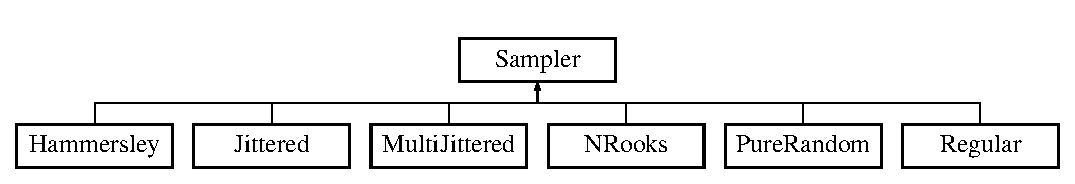
\includegraphics[height=2.000000cm]{class_sampler}
\end{center}
\end{figure}
\subsection*{Public Member Functions}
\begin{DoxyCompactItemize}
\item 
\hyperlink{class_sampler_a9682037ac10546714cfde073143cb0be}{Sampler} ()
\item 
\hyperlink{class_sampler_a8dfadf2352d0c2518c73e54d0b00de39}{Sampler} (const int num\+Samples)
\item 
\hyperlink{class_sampler_ab3d3ec7bbf6be9d8199023d0ad2ec23b}{Sampler} (const int num\+Samples, const int num\+Sets)
\item 
virtual void \hyperlink{class_sampler_a3b75766bf339671a64a05ea9d25cd290}{Generate\+Samples} ()=0
\item 
void \hyperlink{class_sampler_ab6efd9686bab476dbdacbf7922711a45}{Map\+To\+Unit\+Disk} ()
\item 
void \hyperlink{class_sampler_aecad935bae132f108453f9ee5b3d6993}{Map\+To\+Hemisphere} (const float e)
\item 
void \hyperlink{class_sampler_a594169bdbb1673edbd53ec3937841df4}{Setup\+Shuffled\+Indices} ()
\item 
void \hyperlink{class_sampler_afc858c17a6f559d4178e37285eea8f25}{ShuffleX} ()
\item 
void \hyperlink{class_sampler_a685b224ed1cc1a70a0ca602f7b2f6384}{ShuffleY} ()
\item 
glm\+::vec2 \hyperlink{class_sampler_a59fb62883540848f95e3b7655cf18cf6}{Sample\+Unit\+Square} ()
\item 
glm\+::vec2 \hyperlink{class_sampler_aea3eabc2048e29fe920c49aa35957cd5}{Sample\+Unit\+Disk} ()
\item 
glm\+::vec3 \hyperlink{class_sampler_a811c4a50a8767189491e6a5ab7d30cf9}{Sample\+Hemisphere} ()
\item 
int \hyperlink{group___samplers_ga3d438d62d7b7eaec05cff684f96cfe02}{Get\+Num\+Of\+Samples} () const
\end{DoxyCompactItemize}
\subsection*{Protected Member Functions}
\begin{DoxyCompactItemize}
\item 
void \hyperlink{class_sampler_adb58ad84344a6422c6d9096c7f1fabf6}{Set\+Jump} ()
\item 
int \hyperlink{class_sampler_ab0c3297a5b07875a6ddd4215b8aff7b4}{Rand\+Int} ()
\item 
int \hyperlink{class_sampler_a18b4fffc11fe530d4728d89843e975af}{Rand\+Int} (const int min, const int max)
\item 
float \hyperlink{class_sampler_a8adf80273672e0a196298f6d147b9551}{Rand\+Float} ()
\item 
float \hyperlink{class_sampler_ac2ce842ca9597948cbfd175232b5a7a6}{Rand\+Float} (const float min, const float max)
\end{DoxyCompactItemize}
\subsection*{Protected Attributes}
\begin{DoxyCompactItemize}
\item 
int \hyperlink{class_sampler_a8b2c214702841cc163f3cb2a2218284a}{m\+\_\+\+Num\+Samples}
\item 
int \hyperlink{class_sampler_a3a4c91f58f0ddb1d479ae476e689d71e}{m\+\_\+\+Num\+Sets}
\item 
std\+::vector$<$ glm\+::vec2 $>$ \hyperlink{class_sampler_adbc476f6d58621c0ce9173bbe1c53d70}{m\+\_\+\+Samples}
\item 
std\+::vector$<$ glm\+::vec2 $>$ \hyperlink{class_sampler_abb6650869ddaf8002831d257b1b8c426}{m\+\_\+\+Disk\+Samples}
\item 
std\+::vector$<$ glm\+::vec3 $>$ \hyperlink{class_sampler_afd09bd7c820d74c4d658cbef5cb46020}{m\+\_\+\+Hemisphere\+Samples}
\end{DoxyCompactItemize}


\subsection{Detailed Description}
T\+O\+DO \begin{DoxyRemark}{Remarks}
T\+O\+DO. 
\end{DoxyRemark}


\subsection{Constructor \& Destructor Documentation}
\hypertarget{class_sampler_a9682037ac10546714cfde073143cb0be}{}\label{class_sampler_a9682037ac10546714cfde073143cb0be} 
\index{Sampler@{Sampler}!Sampler@{Sampler}}
\index{Sampler@{Sampler}!Sampler@{Sampler}}
\subsubsection{\texorpdfstring{Sampler()}{Sampler()}\hspace{0.1cm}{\footnotesize\ttfamily [1/3]}}
{\footnotesize\ttfamily Sampler\+::\+Sampler (\begin{DoxyParamCaption}{ }\end{DoxyParamCaption})}

Standard constructor. \hypertarget{class_sampler_a8dfadf2352d0c2518c73e54d0b00de39}{}\label{class_sampler_a8dfadf2352d0c2518c73e54d0b00de39} 
\index{Sampler@{Sampler}!Sampler@{Sampler}}
\index{Sampler@{Sampler}!Sampler@{Sampler}}
\subsubsection{\texorpdfstring{Sampler()}{Sampler()}\hspace{0.1cm}{\footnotesize\ttfamily [2/3]}}
{\footnotesize\ttfamily Sampler\+::\+Sampler (\begin{DoxyParamCaption}\item[{const int}]{num\+Samples }\end{DoxyParamCaption})}

Constructs a sampler and sets its number of samples. 
\begin{DoxyParams}{Parameters}
{\em num\+Samples} & Number of samples. \\
\hline
\end{DoxyParams}
\hypertarget{class_sampler_ab3d3ec7bbf6be9d8199023d0ad2ec23b}{}\label{class_sampler_ab3d3ec7bbf6be9d8199023d0ad2ec23b} 
\index{Sampler@{Sampler}!Sampler@{Sampler}}
\index{Sampler@{Sampler}!Sampler@{Sampler}}
\subsubsection{\texorpdfstring{Sampler()}{Sampler()}\hspace{0.1cm}{\footnotesize\ttfamily [3/3]}}
{\footnotesize\ttfamily Sampler\+::\+Sampler (\begin{DoxyParamCaption}\item[{const int}]{num\+Samples,  }\item[{const int}]{num\+Sets }\end{DoxyParamCaption})}

Constructs a sampler and sets its number of samples and sets. 
\begin{DoxyParams}{Parameters}
{\em num\+Samples} & Number of samples. \\
\hline
{\em num\+Sets} & Number of sets. \\
\hline
\end{DoxyParams}


\subsection{Member Function Documentation}
\hypertarget{class_sampler_a3b75766bf339671a64a05ea9d25cd290}{}\label{class_sampler_a3b75766bf339671a64a05ea9d25cd290} 
\index{Sampler@{Sampler}!Generate\+Samples@{Generate\+Samples}}
\index{Generate\+Samples@{Generate\+Samples}!Sampler@{Sampler}}
\subsubsection{\texorpdfstring{Generate\+Samples()}{GenerateSamples()}}
{\footnotesize\ttfamily virtual void Sampler\+::\+Generate\+Samples (\begin{DoxyParamCaption}{ }\end{DoxyParamCaption})\hspace{0.3cm}{\ttfamily [pure virtual]}}

Generates sample patterns in a unit square. \hypertarget{class_sampler_aecad935bae132f108453f9ee5b3d6993}{}\label{class_sampler_aecad935bae132f108453f9ee5b3d6993} 
\index{Sampler@{Sampler}!Map\+To\+Hemisphere@{Map\+To\+Hemisphere}}
\index{Map\+To\+Hemisphere@{Map\+To\+Hemisphere}!Sampler@{Sampler}}
\subsubsection{\texorpdfstring{Map\+To\+Hemisphere()}{MapToHemisphere()}}
{\footnotesize\ttfamily void Sampler\+::\+Map\+To\+Hemisphere (\begin{DoxyParamCaption}\item[{const float}]{e }\end{DoxyParamCaption})}

Maps 2D sample points in the unit square to a hemisphere. 
\begin{DoxyParams}{Parameters}
{\em e} & Controls how the samples are spaced through the hemisphere. \\
\hline
\end{DoxyParams}
\hypertarget{class_sampler_ab6efd9686bab476dbdacbf7922711a45}{}\label{class_sampler_ab6efd9686bab476dbdacbf7922711a45} 
\index{Sampler@{Sampler}!Map\+To\+Unit\+Disk@{Map\+To\+Unit\+Disk}}
\index{Map\+To\+Unit\+Disk@{Map\+To\+Unit\+Disk}!Sampler@{Sampler}}
\subsubsection{\texorpdfstring{Map\+To\+Unit\+Disk()}{MapToUnitDisk()}}
{\footnotesize\ttfamily void Sampler\+::\+Map\+To\+Unit\+Disk (\begin{DoxyParamCaption}{ }\end{DoxyParamCaption})}

Maps 2D sample points in the unit square to a unit disk. \hypertarget{class_sampler_a8adf80273672e0a196298f6d147b9551}{}\label{class_sampler_a8adf80273672e0a196298f6d147b9551} 
\index{Sampler@{Sampler}!Rand\+Float@{Rand\+Float}}
\index{Rand\+Float@{Rand\+Float}!Sampler@{Sampler}}
\subsubsection{\texorpdfstring{Rand\+Float()}{RandFloat()}\hspace{0.1cm}{\footnotesize\ttfamily [1/2]}}
{\footnotesize\ttfamily float Sampler\+::\+Rand\+Float (\begin{DoxyParamCaption}{ }\end{DoxyParamCaption})\hspace{0.3cm}{\ttfamily [protected]}}

Returns a random float with no restrictions. \begin{DoxyReturn}{Returns}
Random float. 
\end{DoxyReturn}
\hypertarget{class_sampler_ac2ce842ca9597948cbfd175232b5a7a6}{}\label{class_sampler_ac2ce842ca9597948cbfd175232b5a7a6} 
\index{Sampler@{Sampler}!Rand\+Float@{Rand\+Float}}
\index{Rand\+Float@{Rand\+Float}!Sampler@{Sampler}}
\subsubsection{\texorpdfstring{Rand\+Float()}{RandFloat()}\hspace{0.1cm}{\footnotesize\ttfamily [2/2]}}
{\footnotesize\ttfamily float Sampler\+::\+Rand\+Float (\begin{DoxyParamCaption}\item[{const float}]{min,  }\item[{const float}]{max }\end{DoxyParamCaption})\hspace{0.3cm}{\ttfamily [protected]}}

Returns a random float within a given range. 
\begin{DoxyParams}{Parameters}
{\em min} & Lower boundary. \\
\hline
{\em max} & Higher boundary. \\
\hline
\end{DoxyParams}
\begin{DoxyReturn}{Returns}
Random float within the range. 
\end{DoxyReturn}
\hypertarget{class_sampler_ab0c3297a5b07875a6ddd4215b8aff7b4}{}\label{class_sampler_ab0c3297a5b07875a6ddd4215b8aff7b4} 
\index{Sampler@{Sampler}!Rand\+Int@{Rand\+Int}}
\index{Rand\+Int@{Rand\+Int}!Sampler@{Sampler}}
\subsubsection{\texorpdfstring{Rand\+Int()}{RandInt()}\hspace{0.1cm}{\footnotesize\ttfamily [1/2]}}
{\footnotesize\ttfamily int Sampler\+::\+Rand\+Int (\begin{DoxyParamCaption}{ }\end{DoxyParamCaption})\hspace{0.3cm}{\ttfamily [protected]}}

Returns a random integer with no restrictions. \begin{DoxyReturn}{Returns}
Random integer. 
\end{DoxyReturn}
\hypertarget{class_sampler_a18b4fffc11fe530d4728d89843e975af}{}\label{class_sampler_a18b4fffc11fe530d4728d89843e975af} 
\index{Sampler@{Sampler}!Rand\+Int@{Rand\+Int}}
\index{Rand\+Int@{Rand\+Int}!Sampler@{Sampler}}
\subsubsection{\texorpdfstring{Rand\+Int()}{RandInt()}\hspace{0.1cm}{\footnotesize\ttfamily [2/2]}}
{\footnotesize\ttfamily int Sampler\+::\+Rand\+Int (\begin{DoxyParamCaption}\item[{const int}]{min,  }\item[{const int}]{max }\end{DoxyParamCaption})\hspace{0.3cm}{\ttfamily [protected]}}

Returns a random integer within a given range. 
\begin{DoxyParams}{Parameters}
{\em min} & Lower boundary. \\
\hline
{\em max} & Higher boundary. \\
\hline
\end{DoxyParams}
\begin{DoxyReturn}{Returns}
Random integer within the range. 
\end{DoxyReturn}
\hypertarget{class_sampler_a811c4a50a8767189491e6a5ab7d30cf9}{}\label{class_sampler_a811c4a50a8767189491e6a5ab7d30cf9} 
\index{Sampler@{Sampler}!Sample\+Hemisphere@{Sample\+Hemisphere}}
\index{Sample\+Hemisphere@{Sample\+Hemisphere}!Sampler@{Sampler}}
\subsubsection{\texorpdfstring{Sample\+Hemisphere()}{SampleHemisphere()}}
{\footnotesize\ttfamily glm\+::vec3 Sampler\+::\+Sample\+Hemisphere (\begin{DoxyParamCaption}{ }\end{DoxyParamCaption})}

Returns a sample in a hemisphere with a random jump. \begin{DoxyReturn}{Returns}
Sample point within a hemisphere. 
\end{DoxyReturn}
\hypertarget{class_sampler_aea3eabc2048e29fe920c49aa35957cd5}{}\label{class_sampler_aea3eabc2048e29fe920c49aa35957cd5} 
\index{Sampler@{Sampler}!Sample\+Unit\+Disk@{Sample\+Unit\+Disk}}
\index{Sample\+Unit\+Disk@{Sample\+Unit\+Disk}!Sampler@{Sampler}}
\subsubsection{\texorpdfstring{Sample\+Unit\+Disk()}{SampleUnitDisk()}}
{\footnotesize\ttfamily glm\+::vec2 Sampler\+::\+Sample\+Unit\+Disk (\begin{DoxyParamCaption}{ }\end{DoxyParamCaption})}

Returns a sample in a unit disk with a random jump. \begin{DoxyReturn}{Returns}
Sample point within a unit disk. 
\end{DoxyReturn}
\hypertarget{class_sampler_a59fb62883540848f95e3b7655cf18cf6}{}\label{class_sampler_a59fb62883540848f95e3b7655cf18cf6} 
\index{Sampler@{Sampler}!Sample\+Unit\+Square@{Sample\+Unit\+Square}}
\index{Sample\+Unit\+Square@{Sample\+Unit\+Square}!Sampler@{Sampler}}
\subsubsection{\texorpdfstring{Sample\+Unit\+Square()}{SampleUnitSquare()}}
{\footnotesize\ttfamily glm\+::vec2 Sampler\+::\+Sample\+Unit\+Square (\begin{DoxyParamCaption}{ }\end{DoxyParamCaption})}

Returns a sample in a unit square with a random jump. \begin{DoxyReturn}{Returns}
Sample point within a unit square. 
\end{DoxyReturn}
\hypertarget{class_sampler_adb58ad84344a6422c6d9096c7f1fabf6}{}\label{class_sampler_adb58ad84344a6422c6d9096c7f1fabf6} 
\index{Sampler@{Sampler}!Set\+Jump@{Set\+Jump}}
\index{Set\+Jump@{Set\+Jump}!Sampler@{Sampler}}
\subsubsection{\texorpdfstring{Set\+Jump()}{SetJump()}}
{\footnotesize\ttfamily void Sampler\+::\+Set\+Jump (\begin{DoxyParamCaption}{ }\end{DoxyParamCaption})\hspace{0.3cm}{\ttfamily [protected]}}

Sets the index jump. \hypertarget{class_sampler_a594169bdbb1673edbd53ec3937841df4}{}\label{class_sampler_a594169bdbb1673edbd53ec3937841df4} 
\index{Sampler@{Sampler}!Setup\+Shuffled\+Indices@{Setup\+Shuffled\+Indices}}
\index{Setup\+Shuffled\+Indices@{Setup\+Shuffled\+Indices}!Sampler@{Sampler}}
\subsubsection{\texorpdfstring{Setup\+Shuffled\+Indices()}{SetupShuffledIndices()}}
{\footnotesize\ttfamily void Sampler\+::\+Setup\+Shuffled\+Indices (\begin{DoxyParamCaption}{ }\end{DoxyParamCaption})}

Sets up randomly shuffled indices for the samples list. \hypertarget{class_sampler_afc858c17a6f559d4178e37285eea8f25}{}\label{class_sampler_afc858c17a6f559d4178e37285eea8f25} 
\index{Sampler@{Sampler}!ShuffleX@{ShuffleX}}
\index{ShuffleX@{ShuffleX}!Sampler@{Sampler}}
\subsubsection{\texorpdfstring{Shuffle\+X()}{ShuffleX()}}
{\footnotesize\ttfamily void Sampler\+::\+ShuffleX (\begin{DoxyParamCaption}{ }\end{DoxyParamCaption})}

Shuffles the X values of the samples list. \hypertarget{class_sampler_a685b224ed1cc1a70a0ca602f7b2f6384}{}\label{class_sampler_a685b224ed1cc1a70a0ca602f7b2f6384} 
\index{Sampler@{Sampler}!ShuffleY@{ShuffleY}}
\index{ShuffleY@{ShuffleY}!Sampler@{Sampler}}
\subsubsection{\texorpdfstring{Shuffle\+Y()}{ShuffleY()}}
{\footnotesize\ttfamily void Sampler\+::\+ShuffleY (\begin{DoxyParamCaption}{ }\end{DoxyParamCaption})}

Shuffles the Y values of the samples list. 

\subsection{Member Data Documentation}
\hypertarget{class_sampler_abb6650869ddaf8002831d257b1b8c426}{}\label{class_sampler_abb6650869ddaf8002831d257b1b8c426} 
\index{Sampler@{Sampler}!m\+\_\+\+Disk\+Samples@{m\+\_\+\+Disk\+Samples}}
\index{m\+\_\+\+Disk\+Samples@{m\+\_\+\+Disk\+Samples}!Sampler@{Sampler}}
\subsubsection{\texorpdfstring{m\+\_\+\+Disk\+Samples}{m\_DiskSamples}}
{\footnotesize\ttfamily std\+::vector$<$glm\+::vec2$>$ Sampler\+::m\+\_\+\+Disk\+Samples\hspace{0.3cm}{\ttfamily [protected]}}

List of sample points within a unit disk. \hypertarget{class_sampler_afd09bd7c820d74c4d658cbef5cb46020}{}\label{class_sampler_afd09bd7c820d74c4d658cbef5cb46020} 
\index{Sampler@{Sampler}!m\+\_\+\+Hemisphere\+Samples@{m\+\_\+\+Hemisphere\+Samples}}
\index{m\+\_\+\+Hemisphere\+Samples@{m\+\_\+\+Hemisphere\+Samples}!Sampler@{Sampler}}
\subsubsection{\texorpdfstring{m\+\_\+\+Hemisphere\+Samples}{m\_HemisphereSamples}}
{\footnotesize\ttfamily std\+::vector$<$glm\+::vec3$>$ Sampler\+::m\+\_\+\+Hemisphere\+Samples\hspace{0.3cm}{\ttfamily [protected]}}

List of sample points within a hemisphere. \hypertarget{class_sampler_a8b2c214702841cc163f3cb2a2218284a}{}\label{class_sampler_a8b2c214702841cc163f3cb2a2218284a} 
\index{Sampler@{Sampler}!m\+\_\+\+Num\+Samples@{m\+\_\+\+Num\+Samples}}
\index{m\+\_\+\+Num\+Samples@{m\+\_\+\+Num\+Samples}!Sampler@{Sampler}}
\subsubsection{\texorpdfstring{m\+\_\+\+Num\+Samples}{m\_NumSamples}}
{\footnotesize\ttfamily int Sampler\+::m\+\_\+\+Num\+Samples\hspace{0.3cm}{\ttfamily [protected]}}

Number of sample points within a set. \hypertarget{class_sampler_a3a4c91f58f0ddb1d479ae476e689d71e}{}\label{class_sampler_a3a4c91f58f0ddb1d479ae476e689d71e} 
\index{Sampler@{Sampler}!m\+\_\+\+Num\+Sets@{m\+\_\+\+Num\+Sets}}
\index{m\+\_\+\+Num\+Sets@{m\+\_\+\+Num\+Sets}!Sampler@{Sampler}}
\subsubsection{\texorpdfstring{m\+\_\+\+Num\+Sets}{m\_NumSets}}
{\footnotesize\ttfamily int Sampler\+::m\+\_\+\+Num\+Sets\hspace{0.3cm}{\ttfamily [protected]}}

Number of sample sets. \hypertarget{class_sampler_adbc476f6d58621c0ce9173bbe1c53d70}{}\label{class_sampler_adbc476f6d58621c0ce9173bbe1c53d70} 
\index{Sampler@{Sampler}!m\+\_\+\+Samples@{m\+\_\+\+Samples}}
\index{m\+\_\+\+Samples@{m\+\_\+\+Samples}!Sampler@{Sampler}}
\subsubsection{\texorpdfstring{m\+\_\+\+Samples}{m\_Samples}}
{\footnotesize\ttfamily std\+::vector$<$glm\+::vec2$>$ Sampler\+::m\+\_\+\+Samples\hspace{0.3cm}{\ttfamily [protected]}}

List of sample points within a unit square. 

The documentation for this class was generated from the following file\+:\begin{DoxyCompactItemize}
\item 
Source/\+Samplers/include/\hyperlink{_sampler_8h}{Sampler.\+h}\end{DoxyCompactItemize}

\hypertarget{class_sphere}{}\section{Sphere Class Reference}
\label{class_sphere}\index{Sphere@{Sphere}}


{\ttfamily \#include $<$Sphere.\+h$>$}

Inheritance diagram for Sphere\+:\begin{figure}[H]
\begin{center}
\leavevmode
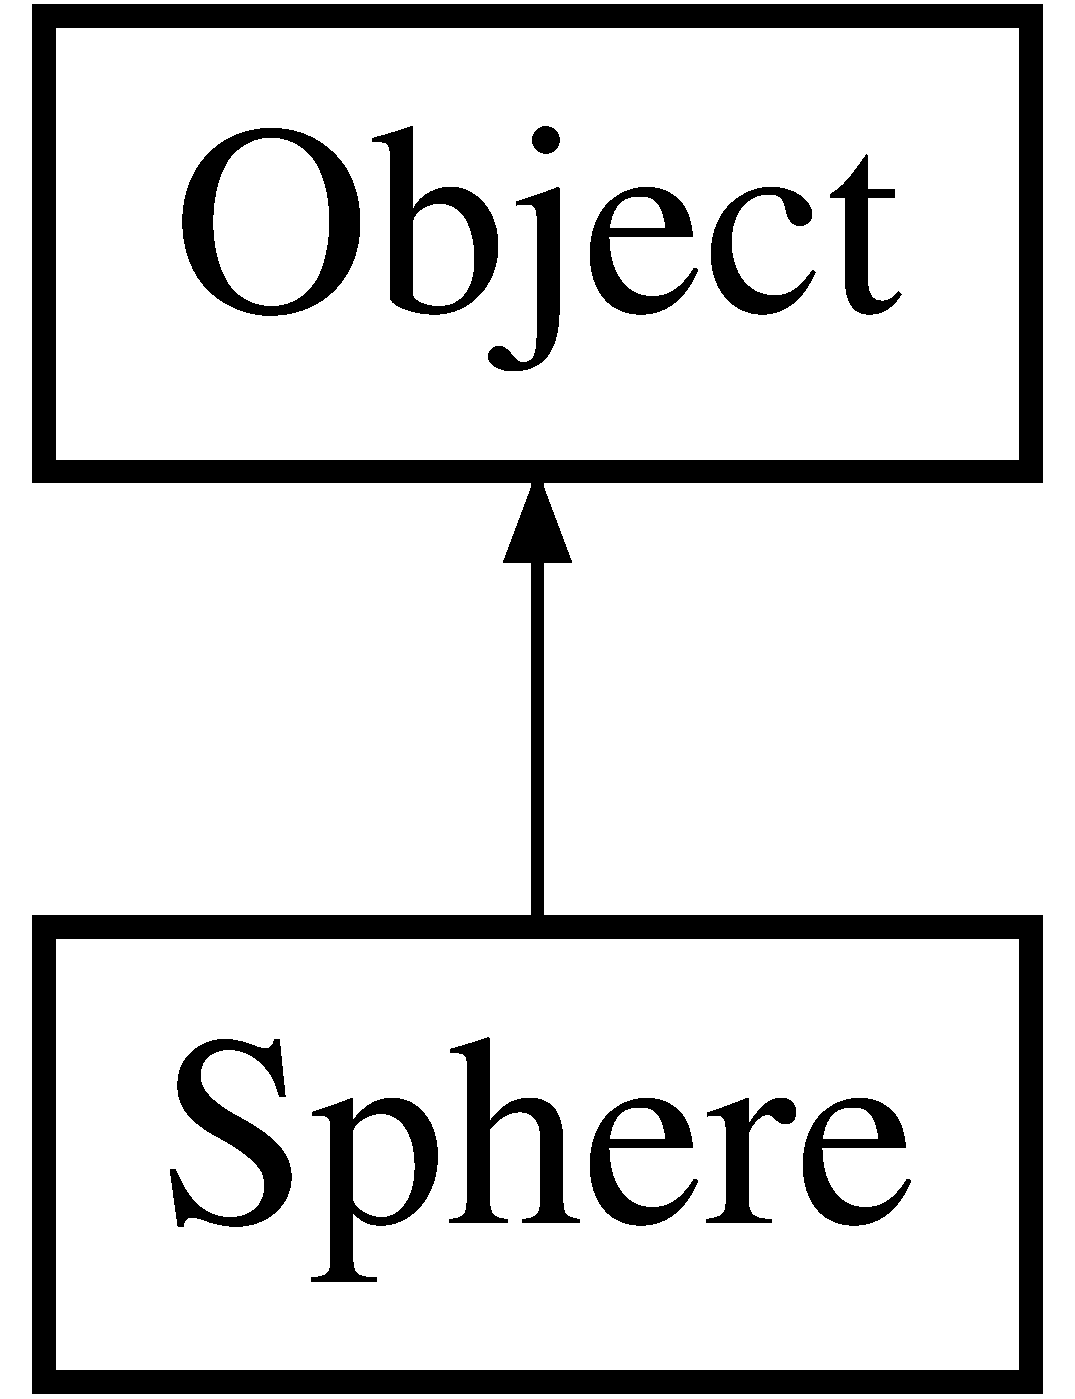
\includegraphics[height=2.000000cm]{class_sphere}
\end{center}
\end{figure}
\subsection*{Public Member Functions}
\begin{DoxyCompactItemize}
\item 
\hyperlink{class_sphere_a890a63ff583cb88e7ec4e840b4ef5eb9}{Sphere} ()
\item 
virtual bool \hyperlink{class_sphere_ab568d3aa3eccdd0c691150fc3d5bb86f}{Hit} (const \hyperlink{class_ray}{Ray} \&ray, double \&tmin, \hyperlink{class_surface}{Surface} \&sr) const
\item 
virtual bool \hyperlink{class_sphere_ac3b3cc027f0cd8c89cecc3b65799267d}{Shadow\+Hit} (const \hyperlink{class_ray}{Ray} \&ray, float \&tmin) const
\item 
void \hyperlink{group___geometric_objects_ga2b8aef309428ea904c75ce3300a71e09}{Set\+Center} (const glm\+::vec3 \&center)
\item 
void \hyperlink{group___geometric_objects_ga0377e69b4a636f542c30c6fa977399e3}{Set\+Radius} (const float radius)
\end{DoxyCompactItemize}
\subsection*{Additional Inherited Members}


\subsection{Detailed Description}
Holder of data of a 3D sphere. \begin{DoxyRemark}{Remarks}
T\+O\+DO. 
\end{DoxyRemark}


\subsection{Constructor \& Destructor Documentation}
\hypertarget{class_sphere_a890a63ff583cb88e7ec4e840b4ef5eb9}{}\label{class_sphere_a890a63ff583cb88e7ec4e840b4ef5eb9} 
\index{Sphere@{Sphere}!Sphere@{Sphere}}
\index{Sphere@{Sphere}!Sphere@{Sphere}}
\subsubsection{\texorpdfstring{Sphere()}{Sphere()}}
{\footnotesize\ttfamily Sphere\+::\+Sphere (\begin{DoxyParamCaption}{ }\end{DoxyParamCaption})}

Standard constructor. 

\subsection{Member Function Documentation}
\hypertarget{class_sphere_ab568d3aa3eccdd0c691150fc3d5bb86f}{}\label{class_sphere_ab568d3aa3eccdd0c691150fc3d5bb86f} 
\index{Sphere@{Sphere}!Hit@{Hit}}
\index{Hit@{Hit}!Sphere@{Sphere}}
\subsubsection{\texorpdfstring{Hit()}{Hit()}}
{\footnotesize\ttfamily virtual bool Sphere\+::\+Hit (\begin{DoxyParamCaption}\item[{const \hyperlink{class_ray}{Ray} \&}]{ray,  }\item[{double \&}]{tmin,  }\item[{\hyperlink{class_surface}{Surface} \&}]{sr }\end{DoxyParamCaption}) const\hspace{0.3cm}{\ttfamily [virtual]}}

Checks if a ray intersects with this object and return it\textquotesingle{}s shading information. 
\begin{DoxyParams}{Parameters}
{\em ray} & Intersection ray. \\
\hline
{\em tmin} & T\+O\+DO. \\
\hline
{\em sr} & Information about the surface of the object. \\
\hline
\end{DoxyParams}
\begin{DoxyReturn}{Returns}
True, if the object intersects with the given ray. 
\end{DoxyReturn}


Implements \hyperlink{class_object_ad9977e40c0a3048eba9a81b25efcf3ef}{Object}.

\hypertarget{class_sphere_ac3b3cc027f0cd8c89cecc3b65799267d}{}\label{class_sphere_ac3b3cc027f0cd8c89cecc3b65799267d} 
\index{Sphere@{Sphere}!Shadow\+Hit@{Shadow\+Hit}}
\index{Shadow\+Hit@{Shadow\+Hit}!Sphere@{Sphere}}
\subsubsection{\texorpdfstring{Shadow\+Hit()}{ShadowHit()}}
{\footnotesize\ttfamily virtual bool Sphere\+::\+Shadow\+Hit (\begin{DoxyParamCaption}\item[{const \hyperlink{class_ray}{Ray} \&}]{ray,  }\item[{float \&}]{tmin }\end{DoxyParamCaption}) const\hspace{0.3cm}{\ttfamily [virtual]}}

Checks if a shadow ray intersects with the object. 
\begin{DoxyParams}{Parameters}
{\em ray} & Shadow ray. \\
\hline
{\em tmin} & T\+O\+DO \\
\hline
\end{DoxyParams}
\begin{DoxyReturn}{Returns}
True, if the object intersects with the given ray. 
\end{DoxyReturn}


Implements \hyperlink{class_object_a020a6edbef7b2591b1dd6815ebbc5aa0}{Object}.



The documentation for this class was generated from the following file\+:\begin{DoxyCompactItemize}
\item 
Source/\+Geometric\+Objects/include/\hyperlink{_sphere_8h}{Sphere.\+h}\end{DoxyCompactItemize}

\hypertarget{class_surface}{}\section{Surface Class Reference}
\label{class_surface}\index{Surface@{Surface}}


{\ttfamily \#include $<$Surface.\+h$>$}

\subsection*{Public Member Functions}
\begin{DoxyCompactItemize}
\item 
\hyperlink{class_surface_a09333b09d58a9c1a23903c5bc21ba425}{Surface} (World \&\hyperlink{class_surface_adc3a6c73b06a4eebb40cc9083d6a956b}{w})
\end{DoxyCompactItemize}
\subsection*{Public Attributes}
\begin{DoxyCompactItemize}
\item 
bool \hyperlink{class_surface_a5fcd1d25c1f67289f4167242c685693c}{m\+\_\+\+Hit}
\item 
std\+::shared\+\_\+ptr$<$ \hyperlink{class_material}{Material} $>$ \hyperlink{class_surface_ac9c3eaa9f8870efbe4cd9e79e28b21e1}{m\+\_\+\+Material\+Ptr}
\item 
glm\+::vec3 \hyperlink{class_surface_ab3cf728434195ae6b569604d90b05bcd}{m\+\_\+\+Hit\+Point}
\item 
glm\+::vec3 \hyperlink{class_surface_ab914f3e5804e0043a140b892e32ab3e7}{m\+\_\+\+Local\+Hit\+Point}
\item 
glm\+::vec3 \hyperlink{class_surface_aa4ae3fc7afb6da10d48beb2bd0590a48}{m\+\_\+\+Normal}
\item 
int \hyperlink{class_surface_a07d2132be1f81e87f7a8d6228e2457c1}{m\+\_\+\+Depth}
\item 
float \hyperlink{class_surface_a19719f48b9ee4fb2a78ef277289f0321}{m\+\_\+T}
\item 
World \& \hyperlink{class_surface_adc3a6c73b06a4eebb40cc9083d6a956b}{w}
\end{DoxyCompactItemize}


\subsection{Detailed Description}
Holds information about a surface. \begin{DoxyRemark}{Remarks}
T\+O\+DO 
\end{DoxyRemark}


\subsection{Constructor \& Destructor Documentation}
\hypertarget{class_surface_a09333b09d58a9c1a23903c5bc21ba425}{}\label{class_surface_a09333b09d58a9c1a23903c5bc21ba425} 
\index{Surface@{Surface}!Surface@{Surface}}
\index{Surface@{Surface}!Surface@{Surface}}
\subsubsection{\texorpdfstring{Surface()}{Surface()}}
{\footnotesize\ttfamily Surface\+::\+Surface (\begin{DoxyParamCaption}\item[{World \&}]{w }\end{DoxyParamCaption})}

Constructs a surface with a reference to the world. 
\begin{DoxyParams}{Parameters}
{\em w} & Reference to the world. \\
\hline
\end{DoxyParams}


\subsection{Member Data Documentation}
\hypertarget{class_surface_a07d2132be1f81e87f7a8d6228e2457c1}{}\label{class_surface_a07d2132be1f81e87f7a8d6228e2457c1} 
\index{Surface@{Surface}!m\+\_\+\+Depth@{m\+\_\+\+Depth}}
\index{m\+\_\+\+Depth@{m\+\_\+\+Depth}!Surface@{Surface}}
\subsubsection{\texorpdfstring{m\+\_\+\+Depth}{m\_Depth}}
{\footnotesize\ttfamily int Surface\+::m\+\_\+\+Depth}

Recursion depth. \hypertarget{class_surface_a5fcd1d25c1f67289f4167242c685693c}{}\label{class_surface_a5fcd1d25c1f67289f4167242c685693c} 
\index{Surface@{Surface}!m\+\_\+\+Hit@{m\+\_\+\+Hit}}
\index{m\+\_\+\+Hit@{m\+\_\+\+Hit}!Surface@{Surface}}
\subsubsection{\texorpdfstring{m\+\_\+\+Hit}{m\_Hit}}
{\footnotesize\ttfamily bool Surface\+::m\+\_\+\+Hit}

Checks if a ray has hit the surface. \hypertarget{class_surface_ab3cf728434195ae6b569604d90b05bcd}{}\label{class_surface_ab3cf728434195ae6b569604d90b05bcd} 
\index{Surface@{Surface}!m\+\_\+\+Hit\+Point@{m\+\_\+\+Hit\+Point}}
\index{m\+\_\+\+Hit\+Point@{m\+\_\+\+Hit\+Point}!Surface@{Surface}}
\subsubsection{\texorpdfstring{m\+\_\+\+Hit\+Point}{m\_HitPoint}}
{\footnotesize\ttfamily glm\+::vec3 Surface\+::m\+\_\+\+Hit\+Point}

Point where the surface has been hit by a ray. \hypertarget{class_surface_ab914f3e5804e0043a140b892e32ab3e7}{}\label{class_surface_ab914f3e5804e0043a140b892e32ab3e7} 
\index{Surface@{Surface}!m\+\_\+\+Local\+Hit\+Point@{m\+\_\+\+Local\+Hit\+Point}}
\index{m\+\_\+\+Local\+Hit\+Point@{m\+\_\+\+Local\+Hit\+Point}!Surface@{Surface}}
\subsubsection{\texorpdfstring{m\+\_\+\+Local\+Hit\+Point}{m\_LocalHitPoint}}
{\footnotesize\ttfamily glm\+::vec3 Surface\+::m\+\_\+\+Local\+Hit\+Point}

Local point where the surface has been hit by a ray. \hypertarget{class_surface_ac9c3eaa9f8870efbe4cd9e79e28b21e1}{}\label{class_surface_ac9c3eaa9f8870efbe4cd9e79e28b21e1} 
\index{Surface@{Surface}!m\+\_\+\+Material\+Ptr@{m\+\_\+\+Material\+Ptr}}
\index{m\+\_\+\+Material\+Ptr@{m\+\_\+\+Material\+Ptr}!Surface@{Surface}}
\subsubsection{\texorpdfstring{m\+\_\+\+Material\+Ptr}{m\_MaterialPtr}}
{\footnotesize\ttfamily std\+::shared\+\_\+ptr$<$\hyperlink{class_material}{Material}$>$ Surface\+::m\+\_\+\+Material\+Ptr}

\hyperlink{class_material}{Material} attached to the surface. \hypertarget{class_surface_aa4ae3fc7afb6da10d48beb2bd0590a48}{}\label{class_surface_aa4ae3fc7afb6da10d48beb2bd0590a48} 
\index{Surface@{Surface}!m\+\_\+\+Normal@{m\+\_\+\+Normal}}
\index{m\+\_\+\+Normal@{m\+\_\+\+Normal}!Surface@{Surface}}
\subsubsection{\texorpdfstring{m\+\_\+\+Normal}{m\_Normal}}
{\footnotesize\ttfamily glm\+::vec3 Surface\+::m\+\_\+\+Normal}

Normal of the surface on the hit point. \hypertarget{class_surface_a19719f48b9ee4fb2a78ef277289f0321}{}\label{class_surface_a19719f48b9ee4fb2a78ef277289f0321} 
\index{Surface@{Surface}!m\+\_\+T@{m\+\_\+T}}
\index{m\+\_\+T@{m\+\_\+T}!Surface@{Surface}}
\subsubsection{\texorpdfstring{m\+\_\+T}{m\_T}}
{\footnotesize\ttfamily float Surface\+::m\+\_\+T}

\hyperlink{class_ray}{Ray} parameter. \hypertarget{class_surface_adc3a6c73b06a4eebb40cc9083d6a956b}{}\label{class_surface_adc3a6c73b06a4eebb40cc9083d6a956b} 
\index{Surface@{Surface}!w@{w}}
\index{w@{w}!Surface@{Surface}}
\subsubsection{\texorpdfstring{w}{w}}
{\footnotesize\ttfamily World\& Surface\+::w}

Reference to the world. 

The documentation for this class was generated from the following file\+:\begin{DoxyCompactItemize}
\item 
Source/\+Utilities/include/\hyperlink{_surface_8h}{Surface.\+h}\end{DoxyCompactItemize}

\hypertarget{class_thin_lens}{}\section{Thin\+Lens Class Reference}
\label{class_thin_lens}\index{Thin\+Lens@{Thin\+Lens}}


{\ttfamily \#include $<$Thin\+Lens.\+h$>$}

Inheritance diagram for Thin\+Lens\+:\begin{figure}[H]
\begin{center}
\leavevmode
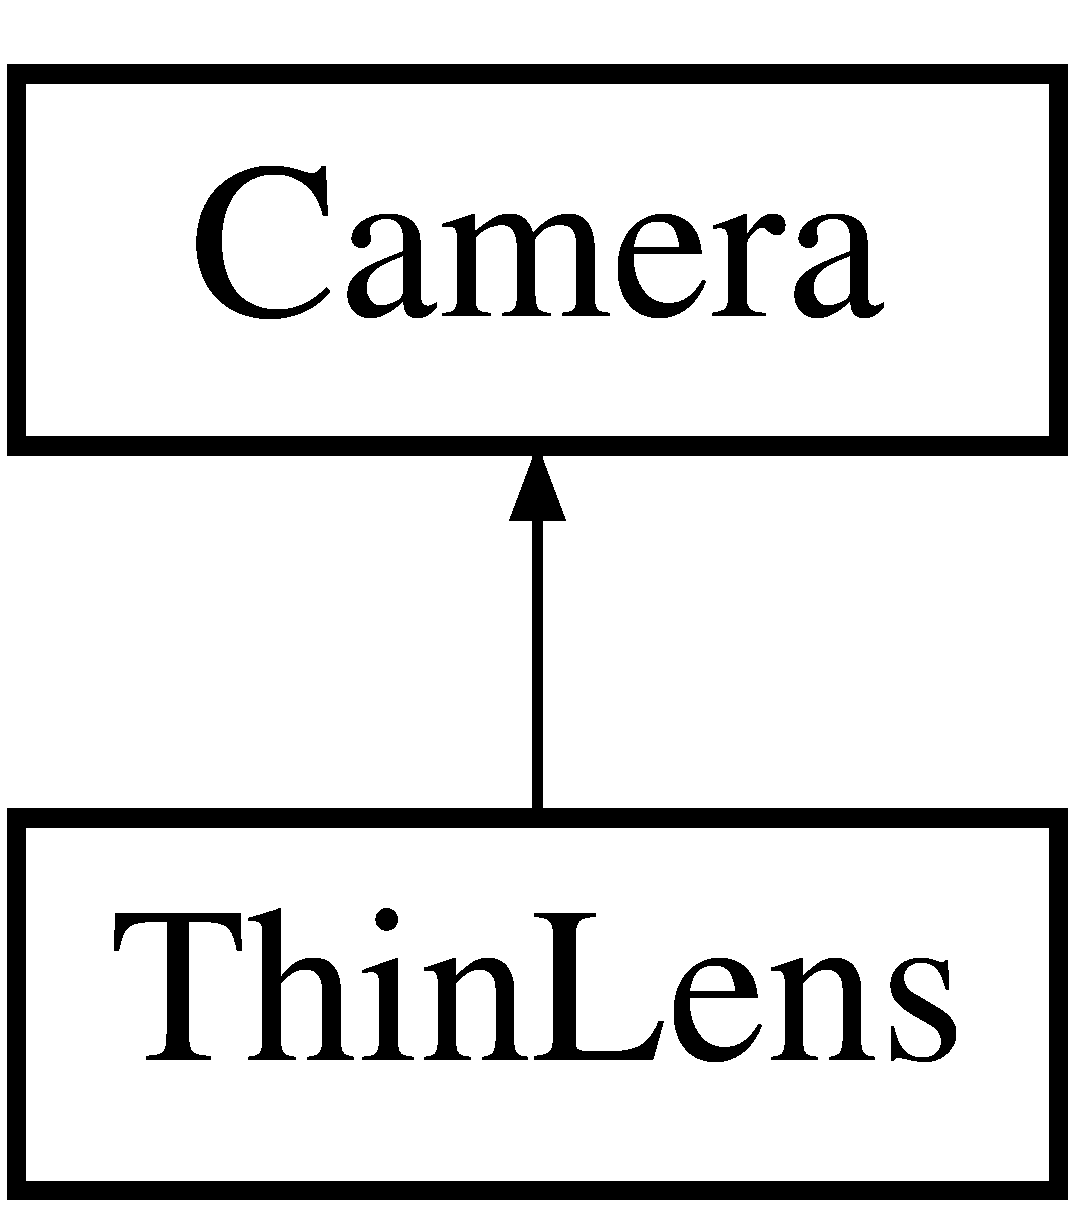
\includegraphics[height=2.000000cm]{class_thin_lens}
\end{center}
\end{figure}
\subsection*{Public Member Functions}
\begin{DoxyCompactItemize}
\item 
\hyperlink{class_thin_lens_ae458cc9405f705ec7c8cbffca08e23b2}{Thin\+Lens} ()
\item 
virtual void \hyperlink{class_thin_lens_af33d499e8fdbdbd196ba3a9b28bdaf5c}{Render\+Scene} (const World \&)
\item 
void \hyperlink{class_thin_lens_acf205ce5a21bd65783c2e67c056664c8}{Set\+Sampler} (std\+::shared\+\_\+ptr$<$ \hyperlink{class_sampler}{Sampler} $>$)
\item 
void \hyperlink{class_thin_lens_a5d4e3ec359df6ebb4dc5163fa48acfc5}{Set\+Lens\+Radius} (const float)
\item 
void \hyperlink{class_thin_lens_a5979bace2e20ea3ede301dff105c403e}{Set\+View\+Plane\+Distance} (const float)
\item 
void \hyperlink{class_thin_lens_a8b14ebeb4fd25147301eba27d8a5530d}{Set\+Focal\+Plane\+Distance} (const float)
\item 
void \hyperlink{class_thin_lens_a10121e3990c0a9bf61394440d2e85421}{Set\+Zoom} (const float)
\end{DoxyCompactItemize}
\subsection*{Additional Inherited Members}


\subsection{Constructor \& Destructor Documentation}
\hypertarget{class_thin_lens_ae458cc9405f705ec7c8cbffca08e23b2}{}\label{class_thin_lens_ae458cc9405f705ec7c8cbffca08e23b2} 
\index{Thin\+Lens@{Thin\+Lens}!Thin\+Lens@{Thin\+Lens}}
\index{Thin\+Lens@{Thin\+Lens}!Thin\+Lens@{Thin\+Lens}}
\subsubsection{\texorpdfstring{Thin\+Lens()}{ThinLens()}}
{\footnotesize\ttfamily Thin\+Lens\+::\+Thin\+Lens (\begin{DoxyParamCaption}{ }\end{DoxyParamCaption})}



\subsection{Member Function Documentation}
\hypertarget{class_thin_lens_af33d499e8fdbdbd196ba3a9b28bdaf5c}{}\label{class_thin_lens_af33d499e8fdbdbd196ba3a9b28bdaf5c} 
\index{Thin\+Lens@{Thin\+Lens}!Render\+Scene@{Render\+Scene}}
\index{Render\+Scene@{Render\+Scene}!Thin\+Lens@{Thin\+Lens}}
\subsubsection{\texorpdfstring{Render\+Scene()}{RenderScene()}}
{\footnotesize\ttfamily virtual void Thin\+Lens\+::\+Render\+Scene (\begin{DoxyParamCaption}\item[{const World \&}]{w }\end{DoxyParamCaption})\hspace{0.3cm}{\ttfamily [virtual]}}

Traces the constructed scene. 
\begin{DoxyParams}{Parameters}
{\em w} & Reference to the world. \\
\hline
\end{DoxyParams}


Implements \hyperlink{class_camera_ad65367e9b225387219d013ffed3f621a}{Camera}.

\hypertarget{class_thin_lens_a8b14ebeb4fd25147301eba27d8a5530d}{}\label{class_thin_lens_a8b14ebeb4fd25147301eba27d8a5530d} 
\index{Thin\+Lens@{Thin\+Lens}!Set\+Focal\+Plane\+Distance@{Set\+Focal\+Plane\+Distance}}
\index{Set\+Focal\+Plane\+Distance@{Set\+Focal\+Plane\+Distance}!Thin\+Lens@{Thin\+Lens}}
\subsubsection{\texorpdfstring{Set\+Focal\+Plane\+Distance()}{SetFocalPlaneDistance()}}
{\footnotesize\ttfamily void Thin\+Lens\+::\+Set\+Focal\+Plane\+Distance (\begin{DoxyParamCaption}\item[{const float}]{fp\+\_\+distance }\end{DoxyParamCaption})\hspace{0.3cm}{\ttfamily [inline]}}

\hypertarget{class_thin_lens_a5d4e3ec359df6ebb4dc5163fa48acfc5}{}\label{class_thin_lens_a5d4e3ec359df6ebb4dc5163fa48acfc5} 
\index{Thin\+Lens@{Thin\+Lens}!Set\+Lens\+Radius@{Set\+Lens\+Radius}}
\index{Set\+Lens\+Radius@{Set\+Lens\+Radius}!Thin\+Lens@{Thin\+Lens}}
\subsubsection{\texorpdfstring{Set\+Lens\+Radius()}{SetLensRadius()}}
{\footnotesize\ttfamily void Thin\+Lens\+::\+Set\+Lens\+Radius (\begin{DoxyParamCaption}\item[{const float}]{lens\+\_\+radius }\end{DoxyParamCaption})\hspace{0.3cm}{\ttfamily [inline]}}

\hypertarget{class_thin_lens_acf205ce5a21bd65783c2e67c056664c8}{}\label{class_thin_lens_acf205ce5a21bd65783c2e67c056664c8} 
\index{Thin\+Lens@{Thin\+Lens}!Set\+Sampler@{Set\+Sampler}}
\index{Set\+Sampler@{Set\+Sampler}!Thin\+Lens@{Thin\+Lens}}
\subsubsection{\texorpdfstring{Set\+Sampler()}{SetSampler()}}
{\footnotesize\ttfamily void Thin\+Lens\+::\+Set\+Sampler (\begin{DoxyParamCaption}\item[{std\+::shared\+\_\+ptr$<$ \hyperlink{class_sampler}{Sampler} $>$}]{ }\end{DoxyParamCaption})}

\hypertarget{class_thin_lens_a5979bace2e20ea3ede301dff105c403e}{}\label{class_thin_lens_a5979bace2e20ea3ede301dff105c403e} 
\index{Thin\+Lens@{Thin\+Lens}!Set\+View\+Plane\+Distance@{Set\+View\+Plane\+Distance}}
\index{Set\+View\+Plane\+Distance@{Set\+View\+Plane\+Distance}!Thin\+Lens@{Thin\+Lens}}
\subsubsection{\texorpdfstring{Set\+View\+Plane\+Distance()}{SetViewPlaneDistance()}}
{\footnotesize\ttfamily void Thin\+Lens\+::\+Set\+View\+Plane\+Distance (\begin{DoxyParamCaption}\item[{const float}]{vp\+\_\+distance }\end{DoxyParamCaption})\hspace{0.3cm}{\ttfamily [inline]}}

\hypertarget{class_thin_lens_a10121e3990c0a9bf61394440d2e85421}{}\label{class_thin_lens_a10121e3990c0a9bf61394440d2e85421} 
\index{Thin\+Lens@{Thin\+Lens}!Set\+Zoom@{Set\+Zoom}}
\index{Set\+Zoom@{Set\+Zoom}!Thin\+Lens@{Thin\+Lens}}
\subsubsection{\texorpdfstring{Set\+Zoom()}{SetZoom()}}
{\footnotesize\ttfamily void Thin\+Lens\+::\+Set\+Zoom (\begin{DoxyParamCaption}\item[{const float}]{zoom }\end{DoxyParamCaption})\hspace{0.3cm}{\ttfamily [inline]}}



The documentation for this class was generated from the following file\+:\begin{DoxyCompactItemize}
\item 
Source/\+Cameras/include/\hyperlink{_thin_lens_8h}{Thin\+Lens.\+h}\end{DoxyCompactItemize}

\hypertarget{class_tracer}{}\section{Tracer Class Reference}
\label{class_tracer}\index{Tracer@{Tracer}}


{\ttfamily \#include $<$Tracer.\+h$>$}

Inheritance diagram for Tracer\+:\begin{figure}[H]
\begin{center}
\leavevmode
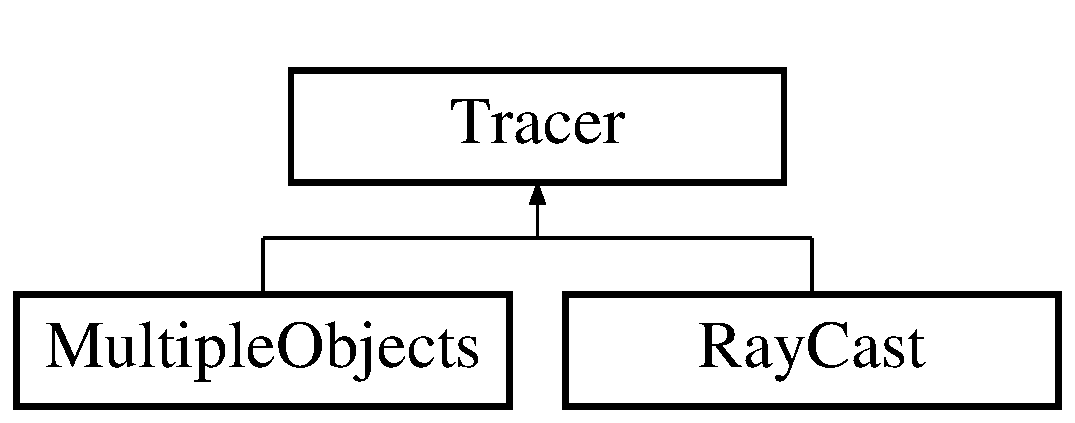
\includegraphics[height=2.000000cm]{class_tracer}
\end{center}
\end{figure}
\subsection*{Public Member Functions}
\begin{DoxyCompactItemize}
\item 
\hyperlink{class_tracer_a0db4955b57c72acfcbb4144f539c5744}{Tracer} (std\+::shared\+\_\+ptr$<$ World $>$ world\+\_\+ptr)
\item 
virtual \hyperlink{class_r_g_b_color}{R\+G\+B\+Color} \hyperlink{class_tracer_adbabdfde11e278945a0433d08445fcce}{Trace\+Ray} (const \hyperlink{class_ray}{Ray} \&ray) const
\end{DoxyCompactItemize}
\subsection*{Protected Attributes}
\begin{DoxyCompactItemize}
\item 
std\+::weak\+\_\+ptr$<$ World $>$ \hyperlink{class_tracer_a0fc389376b5ab36e08fd8e1f6ea16450}{m\+\_\+\+World\+Ptr}
\end{DoxyCompactItemize}


\subsection{Detailed Description}
T\+O\+DO. \begin{DoxyRemark}{Remarks}
T\+O\+DO. 
\end{DoxyRemark}


\subsection{Constructor \& Destructor Documentation}
\hypertarget{class_tracer_a0db4955b57c72acfcbb4144f539c5744}{}\label{class_tracer_a0db4955b57c72acfcbb4144f539c5744} 
\index{Tracer@{Tracer}!Tracer@{Tracer}}
\index{Tracer@{Tracer}!Tracer@{Tracer}}
\subsubsection{\texorpdfstring{Tracer()}{Tracer()}}
{\footnotesize\ttfamily Tracer\+::\+Tracer (\begin{DoxyParamCaption}\item[{std\+::shared\+\_\+ptr$<$ World $>$}]{world\+\_\+ptr }\end{DoxyParamCaption})}

Constructs a \hyperlink{class_tracer}{Tracer} with a pointer to the world. 
\begin{DoxyParams}{Parameters}
{\em world\+\_\+ptr} & Pointer to the world. \\
\hline
\end{DoxyParams}


\subsection{Member Function Documentation}
\hypertarget{class_tracer_adbabdfde11e278945a0433d08445fcce}{}\label{class_tracer_adbabdfde11e278945a0433d08445fcce} 
\index{Tracer@{Tracer}!Trace\+Ray@{Trace\+Ray}}
\index{Trace\+Ray@{Trace\+Ray}!Tracer@{Tracer}}
\subsubsection{\texorpdfstring{Trace\+Ray()}{TraceRay()}}
{\footnotesize\ttfamily virtual \hyperlink{class_r_g_b_color}{R\+G\+B\+Color} Tracer\+::\+Trace\+Ray (\begin{DoxyParamCaption}\item[{const \hyperlink{class_ray}{Ray} \&}]{ray }\end{DoxyParamCaption}) const\hspace{0.3cm}{\ttfamily [virtual]}}

Standard ray tracing method. 
\begin{DoxyParams}{Parameters}
{\em ray} & \hyperlink{class_ray}{Ray} traced. \\
\hline
\end{DoxyParams}
\begin{DoxyReturn}{Returns}
Color of the nearest surface hit by the ray. 
\end{DoxyReturn}


Reimplemented in \hyperlink{class_ray_cast_aed24a822899e5328a7e668a479d3be9e}{Ray\+Cast}, and \hyperlink{class_multiple_objects_a46206cc6dd09a9c587e33ac896bc8e3a}{Multiple\+Objects}.



\subsection{Member Data Documentation}
\hypertarget{class_tracer_a0fc389376b5ab36e08fd8e1f6ea16450}{}\label{class_tracer_a0fc389376b5ab36e08fd8e1f6ea16450} 
\index{Tracer@{Tracer}!m\+\_\+\+World\+Ptr@{m\+\_\+\+World\+Ptr}}
\index{m\+\_\+\+World\+Ptr@{m\+\_\+\+World\+Ptr}!Tracer@{Tracer}}
\subsubsection{\texorpdfstring{m\+\_\+\+World\+Ptr}{m\_WorldPtr}}
{\footnotesize\ttfamily std\+::weak\+\_\+ptr$<$World$>$ Tracer\+::m\+\_\+\+World\+Ptr\hspace{0.3cm}{\ttfamily [protected]}}

Reference to the world. \begin{DoxySeeAlso}{See also}
World 
\end{DoxySeeAlso}


The documentation for this class was generated from the following file\+:\begin{DoxyCompactItemize}
\item 
Source/\+Tracers/include/\hyperlink{_tracer_8h}{Tracer.\+h}\end{DoxyCompactItemize}

\chapter{File Documentation}
\hypertarget{_b_r_d_f_8h}{}\section{Source/\+B\+R\+D\+Fs/include/\+B\+R\+DF.h File Reference}
\label{_b_r_d_f_8h}\index{Source/\+B\+R\+D\+Fs/include/\+B\+R\+D\+F.\+h@{Source/\+B\+R\+D\+Fs/include/\+B\+R\+D\+F.\+h}}
{\ttfamily \#include \char`\"{}Prerequisites.\+h\char`\"{}}\newline
{\ttfamily \#include \char`\"{}R\+G\+B\+Color.\+h\char`\"{}}\newline
\subsection*{Classes}
\begin{DoxyCompactItemize}
\item 
class \hyperlink{class_b_r_d_f}{B\+R\+DF}
\end{DoxyCompactItemize}

\hypertarget{_glossy_specular_8h}{}\section{Source/\+B\+R\+D\+Fs/include/\+Glossy\+Specular.h File Reference}
\label{_glossy_specular_8h}\index{Source/\+B\+R\+D\+Fs/include/\+Glossy\+Specular.\+h@{Source/\+B\+R\+D\+Fs/include/\+Glossy\+Specular.\+h}}
{\ttfamily \#include \char`\"{}B\+R\+D\+F.\+h\char`\"{}}\newline
\subsection*{Classes}
\begin{DoxyCompactItemize}
\item 
class \hyperlink{class_glossy_specular}{Glossy\+Specular}
\end{DoxyCompactItemize}

\hypertarget{_lambertian_8h}{}\section{Source/\+B\+R\+D\+Fs/include/\+Lambertian.h File Reference}
\label{_lambertian_8h}\index{Source/\+B\+R\+D\+Fs/include/\+Lambertian.\+h@{Source/\+B\+R\+D\+Fs/include/\+Lambertian.\+h}}
{\ttfamily \#include \char`\"{}B\+R\+D\+F.\+h\char`\"{}}\newline
\subsection*{Classes}
\begin{DoxyCompactItemize}
\item 
class \hyperlink{class_lambertian}{Lambertian}
\end{DoxyCompactItemize}

\hypertarget{_camera_8h}{}\section{Source/\+Cameras/include/\+Camera.h File Reference}
\label{_camera_8h}\index{Source/\+Cameras/include/\+Camera.\+h@{Source/\+Cameras/include/\+Camera.\+h}}
{\ttfamily \#include \char`\"{}Prerequisites.\+h\char`\"{}}\newline
\subsection*{Classes}
\begin{DoxyCompactItemize}
\item 
class \hyperlink{class_camera}{Camera}
\end{DoxyCompactItemize}

\hypertarget{_orthographic_8h}{}\section{Source/\+Cameras/include/\+Orthographic.h File Reference}
\label{_orthographic_8h}\index{Source/\+Cameras/include/\+Orthographic.\+h@{Source/\+Cameras/include/\+Orthographic.\+h}}
{\ttfamily \#include \char`\"{}Camera.\+h\char`\"{}}\newline
\subsection*{Classes}
\begin{DoxyCompactItemize}
\item 
class \hyperlink{class_orthographic}{Orthographic}
\end{DoxyCompactItemize}

\hypertarget{_pinhole_8h}{}\section{Source/\+Cameras/include/\+Pinhole.h File Reference}
\label{_pinhole_8h}\index{Source/\+Cameras/include/\+Pinhole.\+h@{Source/\+Cameras/include/\+Pinhole.\+h}}
{\ttfamily \#include \char`\"{}Camera.\+h\char`\"{}}\newline
\subsection*{Classes}
\begin{DoxyCompactItemize}
\item 
class \hyperlink{class_pinhole}{Pinhole}
\end{DoxyCompactItemize}

\hypertarget{_thin_lens_8h}{}\section{Source/\+Cameras/include/\+Thin\+Lens.h File Reference}
\label{_thin_lens_8h}\index{Source/\+Cameras/include/\+Thin\+Lens.\+h@{Source/\+Cameras/include/\+Thin\+Lens.\+h}}
{\ttfamily \#include \char`\"{}Camera.\+h\char`\"{}}\newline
\subsection*{Classes}
\begin{DoxyCompactItemize}
\item 
class \hyperlink{class_thin_lens}{Thin\+Lens}
\end{DoxyCompactItemize}

\hypertarget{_object_8h}{}\section{Source/\+Geometric\+Objects/include/\+Object.h File Reference}
\label{_object_8h}\index{Source/\+Geometric\+Objects/include/\+Object.\+h@{Source/\+Geometric\+Objects/include/\+Object.\+h}}
{\ttfamily \#include \char`\"{}Pre\+Requisites.\+h\char`\"{}}\newline
\subsection*{Classes}
\begin{DoxyCompactItemize}
\item 
class \hyperlink{class_object}{Object}
\end{DoxyCompactItemize}

\hypertarget{_plane_8h}{}\section{Source/\+Geometric\+Objects/include/\+Plane.h File Reference}
\label{_plane_8h}\index{Source/\+Geometric\+Objects/include/\+Plane.\+h@{Source/\+Geometric\+Objects/include/\+Plane.\+h}}
{\ttfamily \#include \char`\"{}Object.\+h\char`\"{}}\newline
\subsection*{Classes}
\begin{DoxyCompactItemize}
\item 
class \hyperlink{class_plane}{Plane}
\end{DoxyCompactItemize}

\hypertarget{_sphere_8h}{}\section{Source/\+Geometric\+Objects/include/\+Sphere.h File Reference}
\label{_sphere_8h}\index{Source/\+Geometric\+Objects/include/\+Sphere.\+h@{Source/\+Geometric\+Objects/include/\+Sphere.\+h}}
{\ttfamily \#include \char`\"{}Object.\+h\char`\"{}}\newline
\subsection*{Classes}
\begin{DoxyCompactItemize}
\item 
class \hyperlink{class_sphere}{Sphere}
\end{DoxyCompactItemize}

\hypertarget{_ambient_8h}{}\section{Source/\+Lights/include/\+Ambient.h File Reference}
\label{_ambient_8h}\index{Source/\+Lights/include/\+Ambient.\+h@{Source/\+Lights/include/\+Ambient.\+h}}
{\ttfamily \#include \char`\"{}Light.\+h\char`\"{}}\newline
\subsection*{Classes}
\begin{DoxyCompactItemize}
\item 
class \hyperlink{class_ambient}{Ambient}
\end{DoxyCompactItemize}

\hypertarget{_directional_8h}{}\section{Source/\+Lights/include/\+Directional.h File Reference}
\label{_directional_8h}\index{Source/\+Lights/include/\+Directional.\+h@{Source/\+Lights/include/\+Directional.\+h}}
{\ttfamily \#include \char`\"{}Light.\+h\char`\"{}}\newline
\subsection*{Classes}
\begin{DoxyCompactItemize}
\item 
class \hyperlink{class_directional}{Directional}
\end{DoxyCompactItemize}

\hypertarget{_light_8h}{}\section{Source/\+Lights/include/\+Light.h File Reference}
\label{_light_8h}\index{Source/\+Lights/include/\+Light.\+h@{Source/\+Lights/include/\+Light.\+h}}
{\ttfamily \#include \char`\"{}Prerequisites.\+h\char`\"{}}\newline
{\ttfamily \#include \char`\"{}R\+G\+B\+Color.\+h\char`\"{}}\newline
\subsection*{Classes}
\begin{DoxyCompactItemize}
\item 
class \hyperlink{class_light}{Light}
\end{DoxyCompactItemize}

\hypertarget{_point_light_8h}{}\section{Source/\+Lights/include/\+Point\+Light.h File Reference}
\label{_point_light_8h}\index{Source/\+Lights/include/\+Point\+Light.\+h@{Source/\+Lights/include/\+Point\+Light.\+h}}
{\ttfamily \#include \char`\"{}Light.\+h\char`\"{}}\newline
\subsection*{Classes}
\begin{DoxyCompactItemize}
\item 
class \hyperlink{class_point_light}{Point\+Light}
\end{DoxyCompactItemize}

\hypertarget{_material_8h}{}\section{Source/\+Materials/include/\+Material.h File Reference}
\label{_material_8h}\index{Source/\+Materials/include/\+Material.\+h@{Source/\+Materials/include/\+Material.\+h}}
{\ttfamily \#include \char`\"{}Prerequisites.\+h\char`\"{}}\newline
\subsection*{Classes}
\begin{DoxyCompactItemize}
\item 
class \hyperlink{class_material}{Material}
\end{DoxyCompactItemize}

\hypertarget{_matte_8h}{}\section{Source/\+Materials/include/\+Matte.h File Reference}
\label{_matte_8h}\index{Source/\+Materials/include/\+Matte.\+h@{Source/\+Materials/include/\+Matte.\+h}}
{\ttfamily \#include \char`\"{}Material.\+h\char`\"{}}\newline
{\ttfamily \#include \char`\"{}Lambertian.\+h\char`\"{}}\newline
\subsection*{Classes}
\begin{DoxyCompactItemize}
\item 
class \hyperlink{class_matte}{Matte}
\end{DoxyCompactItemize}

\hypertarget{_phong_8h}{}\section{Source/\+Materials/include/\+Phong.h File Reference}
\label{_phong_8h}\index{Source/\+Materials/include/\+Phong.\+h@{Source/\+Materials/include/\+Phong.\+h}}
{\ttfamily \#include \char`\"{}Material.\+h\char`\"{}}\newline
{\ttfamily \#include \char`\"{}Lambertian.\+h\char`\"{}}\newline
{\ttfamily \#include \char`\"{}Glossy\+Specular.\+h\char`\"{}}\newline
\subsection*{Classes}
\begin{DoxyCompactItemize}
\item 
class \hyperlink{class_phong}{Phong}
\end{DoxyCompactItemize}

\hypertarget{_hammersley_8h}{}\section{Source/\+Samplers/include/\+Hammersley.h File Reference}
\label{_hammersley_8h}\index{Source/\+Samplers/include/\+Hammersley.\+h@{Source/\+Samplers/include/\+Hammersley.\+h}}
{\ttfamily \#include \char`\"{}Sampler.\+h\char`\"{}}\newline
\subsection*{Classes}
\begin{DoxyCompactItemize}
\item 
class \hyperlink{class_hammersley}{Hammersley}
\end{DoxyCompactItemize}

\hypertarget{_jittered_8h}{}\section{Source/\+Samplers/include/\+Jittered.h File Reference}
\label{_jittered_8h}\index{Source/\+Samplers/include/\+Jittered.\+h@{Source/\+Samplers/include/\+Jittered.\+h}}
{\ttfamily \#include \char`\"{}Sampler.\+h\char`\"{}}\newline
\subsection*{Classes}
\begin{DoxyCompactItemize}
\item 
class \hyperlink{class_jittered}{Jittered}
\end{DoxyCompactItemize}

\hypertarget{_multi_jittered_8h}{}\section{Source/\+Samplers/include/\+Multi\+Jittered.h File Reference}
\label{_multi_jittered_8h}\index{Source/\+Samplers/include/\+Multi\+Jittered.\+h@{Source/\+Samplers/include/\+Multi\+Jittered.\+h}}
{\ttfamily \#include \char`\"{}Sampler.\+h\char`\"{}}\newline
\subsection*{Classes}
\begin{DoxyCompactItemize}
\item 
class \hyperlink{class_multi_jittered}{Multi\+Jittered}
\end{DoxyCompactItemize}

\hypertarget{_n_rooks_8h}{}\section{Source/\+Samplers/include/\+N\+Rooks.h File Reference}
\label{_n_rooks_8h}\index{Source/\+Samplers/include/\+N\+Rooks.\+h@{Source/\+Samplers/include/\+N\+Rooks.\+h}}
{\ttfamily \#include \char`\"{}Sampler.\+h\char`\"{}}\newline
\subsection*{Classes}
\begin{DoxyCompactItemize}
\item 
class \hyperlink{class_n_rooks}{N\+Rooks}
\end{DoxyCompactItemize}

\hypertarget{_pure_random_8h}{}\section{Source/\+Samplers/include/\+Pure\+Random.h File Reference}
\label{_pure_random_8h}\index{Source/\+Samplers/include/\+Pure\+Random.\+h@{Source/\+Samplers/include/\+Pure\+Random.\+h}}
{\ttfamily \#include \char`\"{}Sampler.\+h\char`\"{}}\newline
\subsection*{Classes}
\begin{DoxyCompactItemize}
\item 
class \hyperlink{class_pure_random}{Pure\+Random}
\end{DoxyCompactItemize}

\hypertarget{_regular_8h}{}\section{Source/\+Samplers/include/\+Regular.h File Reference}
\label{_regular_8h}\index{Source/\+Samplers/include/\+Regular.\+h@{Source/\+Samplers/include/\+Regular.\+h}}
{\ttfamily \#include \char`\"{}Sampler.\+h\char`\"{}}\newline
\subsection*{Classes}
\begin{DoxyCompactItemize}
\item 
class \hyperlink{class_regular}{Regular}
\end{DoxyCompactItemize}

\hypertarget{_sampler_8h}{}\section{Source/\+Samplers/include/\+Sampler.h File Reference}
\label{_sampler_8h}\index{Source/\+Samplers/include/\+Sampler.\+h@{Source/\+Samplers/include/\+Sampler.\+h}}
{\ttfamily \#include \char`\"{}Prerequisites.\+h\char`\"{}}\newline
\subsection*{Classes}
\begin{DoxyCompactItemize}
\item 
class \hyperlink{class_sampler}{Sampler}
\end{DoxyCompactItemize}

\hypertarget{_multiple_objects_8h}{}\section{Source/\+Tracers/include/\+Multiple\+Objects.h File Reference}
\label{_multiple_objects_8h}\index{Source/\+Tracers/include/\+Multiple\+Objects.\+h@{Source/\+Tracers/include/\+Multiple\+Objects.\+h}}
{\ttfamily \#include \char`\"{}Tracer.\+h\char`\"{}}\newline
\subsection*{Classes}
\begin{DoxyCompactItemize}
\item 
class \hyperlink{class_multiple_objects}{Multiple\+Objects}
\end{DoxyCompactItemize}

\hypertarget{_ray_cast_8h}{}\section{Source/\+Tracers/include/\+Ray\+Cast.h File Reference}
\label{_ray_cast_8h}\index{Source/\+Tracers/include/\+Ray\+Cast.\+h@{Source/\+Tracers/include/\+Ray\+Cast.\+h}}
{\ttfamily \#include \char`\"{}Tracer.\+h\char`\"{}}\newline
\subsection*{Classes}
\begin{DoxyCompactItemize}
\item 
class \hyperlink{class_ray_cast}{Ray\+Cast}
\end{DoxyCompactItemize}

\hypertarget{_tracer_8h}{}\section{Source/\+Tracers/include/\+Tracer.h File Reference}
\label{_tracer_8h}\index{Source/\+Tracers/include/\+Tracer.\+h@{Source/\+Tracers/include/\+Tracer.\+h}}
{\ttfamily \#include \char`\"{}Prerequisites.\+h\char`\"{}}\newline
\subsection*{Classes}
\begin{DoxyCompactItemize}
\item 
class \hyperlink{class_tracer}{Tracer}
\end{DoxyCompactItemize}

\hypertarget{_logger_8h}{}\section{Source/\+Utilities/include/\+Logger.h File Reference}
\label{_logger_8h}\index{Source/\+Utilities/include/\+Logger.\+h@{Source/\+Utilities/include/\+Logger.\+h}}
{\ttfamily \#include \char`\"{}Prerequisites.\+h\char`\"{}}\newline
\subsection*{Namespaces}
\begin{DoxyCompactItemize}
\item 
 \hyperlink{namespace_logger}{Logger}
\end{DoxyCompactItemize}
\subsection*{Enumerations}
\begin{DoxyCompactItemize}
\item 
enum \hyperlink{namespace_logger_a8f625bd9ec5f706cb67b725a98743c04}{Logger\+::\+Log\+Type} \{ \hyperlink{namespace_logger_a8f625bd9ec5f706cb67b725a98743c04ab46e195aa1062a5d9f4366486ea131f3}{Logger\+::\+L\+T\+\_\+\+D\+E\+B\+UG}, 
\hyperlink{namespace_logger_a8f625bd9ec5f706cb67b725a98743c04a7558ebf8aecb9a3b538e639e11237f33}{Logger\+::\+L\+T\+\_\+\+E\+R\+R\+OR}, 
\hyperlink{namespace_logger_a8f625bd9ec5f706cb67b725a98743c04ae2f929c9ea7ffc45e696e247034a1616}{Logger\+::\+L\+T\+\_\+\+I\+N\+FO}
 \}
\item 
enum \hyperlink{namespace_logger_a5838bb966bb2e56b838cbf5ce207d014}{Logger\+::\+Log\+Detail} \{ \hyperlink{namespace_logger_a5838bb966bb2e56b838cbf5ce207d014a13b85f16e10f02f0f7831f7f1e62172e}{Logger\+::\+L\+D\+\_\+\+L\+I\+T\+T\+LE}, 
\hyperlink{namespace_logger_a5838bb966bb2e56b838cbf5ce207d014acdb9720161dbe34ef066448bc3362452}{Logger\+::\+L\+D\+\_\+\+N\+O\+R\+M\+AL}, 
\hyperlink{namespace_logger_a5838bb966bb2e56b838cbf5ce207d014a81011f9c7cb8f58acfae6d88b064466b}{Logger\+::\+L\+D\+\_\+\+H\+I\+GH}
 \}
\item 
enum \hyperlink{namespace_logger_ac0ba8933d14b2c05d8a87ef9319924fa}{Logger\+::\+Log\+Relevance} \{ \hyperlink{namespace_logger_ac0ba8933d14b2c05d8a87ef9319924faaae660d03b3378eb8cf44d6acc5f03734}{Logger\+::\+L\+R\+\_\+\+T\+R\+I\+V\+I\+AL}, 
\hyperlink{namespace_logger_ac0ba8933d14b2c05d8a87ef9319924faa4427eed1049860091a1cd794be6817cf}{Logger\+::\+L\+R\+\_\+\+N\+O\+R\+M\+AL}, 
\hyperlink{namespace_logger_ac0ba8933d14b2c05d8a87ef9319924faa34fddfe05472d43cf2f67c5ecae54d57}{Logger\+::\+L\+R\+\_\+\+I\+M\+P\+O\+R\+T\+A\+NT}
 \}
\end{DoxyCompactItemize}
\subsection*{Functions}
\begin{DoxyCompactItemize}
\item 
void \hyperlink{namespace_logger_aea870326f4476cc49457cfdcc6256022}{Logger\+::\+Start\+Log} ()
\item 
void \hyperlink{namespace_logger_a6506657f7b715f4ed4de8545c9b44e44}{Logger\+::\+Log} (Log\+Type type, std\+::string message, std\+::string component)
\item 
void \hyperlink{namespace_logger_a9e0df3839eb703f75a748ab42ffe55da}{Logger\+::\+Debug\+Log} (std\+::string message, std\+::string component)
\item 
void \hyperlink{namespace_logger_a8b60f8445102c57b2f133cf523646e43}{Logger\+::\+Error\+Log} (std\+::string message, std\+::string component)
\item 
void \hyperlink{namespace_logger_ad751d2237527a66a0a7191d784a945a8}{Logger\+::\+Info\+Log} (std\+::string message, std\+::string component)
\item 
void \hyperlink{namespace_logger_a6e44b3fec519cb3bd99514d00170ef4b}{Logger\+::\+Save\+Log} ()
\end{DoxyCompactItemize}

\hypertarget{_ray_8h}{}\section{Source/\+Utilities/include/\+Ray.h File Reference}
\label{_ray_8h}\index{Source/\+Utilities/include/\+Ray.\+h@{Source/\+Utilities/include/\+Ray.\+h}}
{\ttfamily \#include \char`\"{}Prerequisites.\+h\char`\"{}}\newline
\subsection*{Classes}
\begin{DoxyCompactItemize}
\item 
class \hyperlink{class_ray}{Ray}
\end{DoxyCompactItemize}

\hypertarget{_r_g_b_color_8h}{}\section{Source/\+Utilities/include/\+R\+G\+B\+Color.h File Reference}
\label{_r_g_b_color_8h}\index{Source/\+Utilities/include/\+R\+G\+B\+Color.\+h@{Source/\+Utilities/include/\+R\+G\+B\+Color.\+h}}
{\ttfamily \#include \char`\"{}Prerequisites.\+h\char`\"{}}\newline
\subsection*{Classes}
\begin{DoxyCompactItemize}
\item 
class \hyperlink{class_r_g_b_color}{R\+G\+B\+Color}
\end{DoxyCompactItemize}

\hypertarget{_surface_8h}{}\section{Source/\+Utilities/include/\+Surface.h File Reference}
\label{_surface_8h}\index{Source/\+Utilities/include/\+Surface.\+h@{Source/\+Utilities/include/\+Surface.\+h}}
{\ttfamily \#include \char`\"{}Prerequisites.\+h\char`\"{}}\newline
{\ttfamily \#include \char`\"{}Ray.\+h\char`\"{}}\newline
{\ttfamily \#include \char`\"{}R\+G\+B\+Color.\+h\char`\"{}}\newline
\subsection*{Classes}
\begin{DoxyCompactItemize}
\item 
class \hyperlink{class_surface}{Surface}
\end{DoxyCompactItemize}

%--- End generated contents ---

% Index
\backmatter
\newpage
\phantomsection
\clearemptydoublepage
\addcontentsline{toc}{chapter}{Index}
\printindex

\end{document}
